\documentclass[DIV=calc, paper=a4, fontsize=11pt, twocolumn]{scrartcl}	 % A4 paper and 11pt font size
\usepackage{graphicx}
\usepackage{subcaption} % Required for the subfigure environment
\usepackage{longtable}
\usepackage{lipsum} % Used for inserting dummy 'Lorem ipsum' text into the template
\usepackage[english]{babel} % English language/hyphenation
\usepackage[protrusion=true,expansion=true]{microtype} % Better typography
\usepackage{amsmath,amsfonts,amsthm} % Math packages
\usepackage[svgnames]{xcolor} % Enabling colors by their 'svgnames'
\usepackage{booktabs} % Horizontal rules in tables
\usepackage[font=small,labelfont=bf,textfont=it]{caption}
\usepackage{fix-cm}	 % Custom font sizes - used for the initial letter in the document
\usepackage{graphicx} % Package to insert images
\usepackage{hyperref}
\usepackage{amssymb}
\usepackage{fancyhdr} % Needed to define custom headers/footers
\pagestyle{fancy} % Enables the custom headers/footers
\usepackage{lastpage} % Used to determine the number of pages in the document (for "Page X of Total")
\usepackage{comment}
\usepackage{booktabs}
\lhead{\small Bridgeless Boost PFC Converter}
\rhead{\rightmark}
\renewcommand{\headrulewidth}{0.4pt}
% Footers
\cfoot{\footnotesize \thepage} 
\renewcommand{\sectionmark}[1]{\markright{\thesection\ #1}}
% \renewcommand{\headrulewidth}{0.0pt} % No header rule
\renewcommand{\footrulewidth}{0.4pt} % Thin footer rule
% --- Replaced unicode-math with standard pdfLaTeX compatible fonts ---
\usepackage[T1]{fontenc}
\usepackage{tgpagella} 
\usepackage{amsmath}
% ---------------------------------------------------------------------

\usepackage{siunitx}
\usepackage{xcolor}
\usepackage{booktabs,colortbl, array}
\usepackage{pgfplotstable}
\pgfplotsset{compat=1.8}

\definecolor{rulecolor}{RGB}{0,71,171}
\definecolor{tableheadcolor}{gray}{0.92}

\newcommand{\topline}{ %
        \arrayrulecolor{rulecolor}\specialrule{0.1em}{\abovetopsep}{0pt}%
        \arrayrulecolor{tableheadcolor}\specialrule{\belowrulesep}{0pt}{0pt}%
        \arrayrulecolor{rulecolor}}
\newcommand{\midtopline}{ %
        \arrayrulecolor{tableheadcolor}\specialrule{\aboverulesep}{0pt}{0pt}%
        \arrayrulecolor{rulecolor}\specialrule{\lightrulewidth}{0pt}{0pt}%
        \arrayrulecolor{white}\specialrule{\belowrulesep}{0pt}{0pt}%
        \arrayrulecolor{rulecolor}}
\newcommand{\bottomline}{ %
        \arrayrulecolor{white}\specialrule{\aboverulesep}{0pt}{0pt}%
        \arrayrulecolor{rulecolor} %
        \specialrule{\heavyrulewidth}{0pt}{\belowbottomsep}}%

\newcommand{\midheader}[2]{%
        \midrule\topmidheader{#1}{#2}}
\newcommand\topmidheader[2]{\multicolumn{#1}{c}{\textsc{#2}}\\%
        \addlinespace[0.5ex]}

\pgfplotstableset{normal/.style ={%
        header=true,
        string type,
        font=\small, % <--- Removed the broken fontspec command here
        column type=l,
        every odd row/.style={
            before row=
        },
        every head row/.style={
            before row={\topline\rowcolor{tableheadcolor}},
            after row={\midtopline}
        },
        every last row/.style={
            after row=\bottomline
        },
        col sep=&,
        row sep=\\
    }
}
\usepackage{lettrine} % Package to accentuate the first letter of the text
\newcommand{\initial}[1]{ % Defines the command and style for the first letter
\lettrine[lines=3,lhang=0.3,nindent=0em]{
\color{Black}
{\textsf{#1}}}{}}


%----------------------------------------------------------------------------------------
%    TITLE SECTION
%----------------------------------------------------------------------------------------

\usepackage{titling} % Allows custom title configuration

\newcommand{\HorRule}{\color{Black} \rule{\linewidth}{1pt}} % Defines the gold horizontal rule around the title

% Use \raggedright instead of \begin{flushleft} to avoid breaking scope boundaries.
% Also fixed \fontsize{20}{5} to \fontsize{20}{24} so multi-line titles don't overlap.
\pretitle{\vspace{-30pt} \raggedright \HorRule \vspace{10pt} \fontsize{20}{24} \usefont{OT1}{phv}{b}{n} \color{Black} \selectfont} 

% Lab Report Title Goes Here
\title{Bridgeless Boost PFC Converter: Control Strategies Comparison} 
% Lab Report Title Goes Here

\posttitle{\par \vspace{15pt}} % Whitespace under the title

% Changed to \centering to allow the 3 columns to center properly on the page
\preauthor{\centering \large \usefont{OT1}{phv}{m}{n} \color{Black}} % Author font configuration
\author{
    \vspace{-10pt}
    \small 
    \begin{tabular}[t]{c}
        \textbf{Antonio Pedicini} \\
        (389000080) \\
        \href{mailto:a.pedicini8@studenti.unisannio.it}{a.pedicini8@studenti.unisannio.it}
    \end{tabular}
    \hfill
    \begin{tabular}[t]{c}
        \textbf{Marco Vaccarella} \\
        (389000051) \\
        \href{mailto:m.vaccarella2@studenti.unisannio.it}{m.vaccarella2@studenti.unisannio.it}
    \end{tabular}
    \hfill
    \begin{tabular}[t]{c}
        \textbf{Marco Pizzulo} \\
        (389000084) \\
        \href{mailto:m.pizzulo2@studenti.unisannio.it}{m.pizzulo2@studenti.unisannio.it}
    \end{tabular}
}

% Removed the lengthy postauthor text since affiliations are now in the author block
\postauthor{
    \par \vspace{15pt} 
    \footnotesize \usefont{OT1}{phv}{m}{sl} \color{Black} 
    Prof. Luigi Iannelli, Dynamics and Control of Switched Electronic Systems\\
    
    Master's Degree in Electronics Engineering for Automation and Sensing, \\ 
    Università degli Studi del Sannio, Benevento, Italy, 82100
    \par \vspace{10pt} \HorRule
}

\date{May 5, 2026}

%----------------------------------------------------------------------------------------

\begin{document}

\maketitle % Print the title

\thispagestyle{empty} % Enabling the custom headers/footers for the second page forward

%----------------------------------------------------------------------------------------
%	ABSTRACT
%----------------------------------------------------------------------------------------

% The first character should be within \initial{}
\initial{T}\textbf{he performance of three distinct control strategies for the Bridgeless Boost PFC Converter (BBC) is evaluated.% The first two strategies are the cascaded PI/PR and the Lyapunov-based inner control loop solutions; the third, the dynamic phasors approach, instead uses an SOGI-PLL that independently governs the direct and quadrature control components.%
The three strategies use a PI controller in the external loop, which generates the current reference from the output voltage error. 
The difference of the three strategies is in the internal loop used for stablize the system using the input inductor current. 
The internal loop controllers are: Lyapunov-based inner control, PR controller, and phasor-domain approach to model two inner PI control loops for the quadrature and direct-current components. 
First, the converter's analytical model is analyzed using averaged and small-signal modeling techniques. Following a detailed theoretical examination of each control scheme, a comprehensive comparative evaluation is conducted using PLECS simulations.}

%----------------------------------------------------------------------------------------
%	ARTICLE CONTENTS
%----------------------------------------------------------------------------------------

\section*{Introduction}

Single-phase AC/DC Power Factor Correction (PFC) converters function as full-wave controlled rectifiers in power electronics, delivering high efficiency and enhanced power quality \cite{survey_topologies}. Without PFC circuits, grid current and voltage fall out of phase \cite{TU}, which increases reactive power and consequently degrades overall system efficiency and power quality. Power factor measures the efficiency of a load's AC power consumption; a high power factor indicates optimal energy utilization, whereas a low, leading, or lagging power factor causes transmission losses and poor efficiency. A common way to define the PF is the following:
\begin{equation}
	PF = \frac{P_{AV}}{V_{RMS} I_{RMS}}
\end{equation}
where \textbf{$P_{AV}$} is the real power, and the product \textbf{$V_{RMS} I_{RMS}$} represents apparent power. An alternative form of the PF definition is:
\begin{equation}
	PF = \frac{I_{1_{RMS}}}{I_{RMS}} \cos{\phi}
\end{equation}
where \textbf{$I_{1_{RMS}}$} is the Root Mean Square (RMS) value of the fundamental component of the current (the part at Mains frequency), \textbf{$I_{RMS}$} is the total RMS current, which includes the fundamental frequency plus all harmonic distortions, and \textbf{$\cos{\phi}$} is the phase difference between the voltage and the fundamental current component.

The relationship between the Power Factor and the Total Harmonic Distortion (THD) can be explicitly established from this second definition. By expressing the total RMS current as a function of its fundamental component and the accumulated harmonic distortion, the ratio $\frac{I_{1_{RMS}}}{I_{RMS}}$ can be mathematically rewritten as $\frac{1}{\sqrt{1 + \text{THD}^2}}$. Consequently, the complete Power Factor expression becomes:
\begin{equation}
    PF = \frac{1}{\sqrt{1 + \text{THD}^2}} \cos{\phi}
\end{equation}
In properly controlled PFC converters, the control loop forces the input current to be perfectly in phase with the grid voltage, driving the displacement factor ($\cos{\phi}$) to near unity. Under these optimal conditions, the Power Factor becomes almost entirely dependent on the harmonic content ($PF \approx \frac{1}{\sqrt{1 + \text{THD}^2}}$), demonstrating that minimizing the THD is strictly necessary to maximize the overall Power Factor.

In the existing literature, various types of single‐phase PFC converters have been presented that are essentially derived from conventional boost and buck/boost converters with a bridge rectifier. Bridge-boost topology is the most common for PFC applications. It uses a dedicated diode bridge to rectify the AC input voltage to DC, which is then followed by the boost section \cite{MG}. The nonlinear nature of bridge rectifiers causes non-sinusoidal current draw and injects grid harmonics, leading to voltage distortion, heating, and noise that degrade overall power system efficiency \cite{MG}.

\begin{figure}
  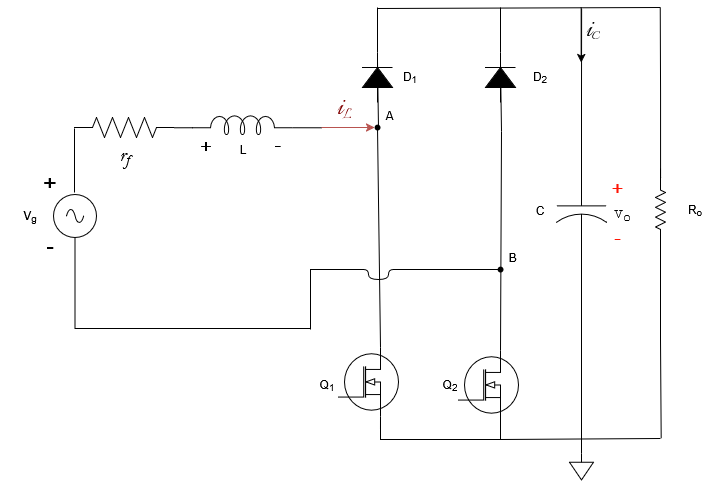
\includegraphics[width=\linewidth]{figures/bridgeless.png}
  \caption{Bridgeless Boost PFC Converter.}
  \label{fig:bridgeless-pfc}
\end{figure}

By eliminating the grid-side diode bridge, the bridgeless boost PFC circuit achieves a smaller footprint and lower power losses than traditional systems; however, its floating input voltage relative to the PFC stage necessitates isolated circuitry for precise measurement \cite{TU}. The conventional bridgless boost PFC converter topology is shown in Figure \ref{fig:bridgeless-pfc}.

The standard PFC control strategy is typically implemented using a cascaded dual-loop architecture: a fast internal current loop designed to shape the grid current to achieve near-unity PF, and a slow external voltage loop to regulate and stabilize the DC output voltage. Nevertheless, implementing the inner current loop with standard Linear Time-Invariant (LTI) Proportional-Integral (PI) controllers in the stationary AC frame inevitably introduces steady-state phase and amplitude tracking errors, as LTI controllers lack infinite gain at the sinusoidal reference frequency \cite{pr_pfc}. Consequently, advanced control paradigms are increasingly adopted to overcome these limitations. Proportional-Resonant (PR) compensators introduce an infinite theoretical gain precisely at the fundamental grid frequency to ensure zero steady-state error \cite{pr_control, pr_pfc}. Alternatively, phasors domain modelling and control maps the AC variables into DC-equivalent components, allowing standard PI controllers to operate on mathematically flat references extracted via Phase-Locked Loops (PLL) \cite{totem_pole_dq}. Finally, non-linear Lyapunov-based control strategies can be utilized to guarantee global asymptotic stability and fast transient response without relying on linear LTI approximations \cite{TU, lyapunov_pr}.

\section{Operating Modes}

This section presents the operating principle and mathematical model of the BBC. This model represents the relationship of physical variables in the power converter.

\begin{figure}[h]
    \centering
    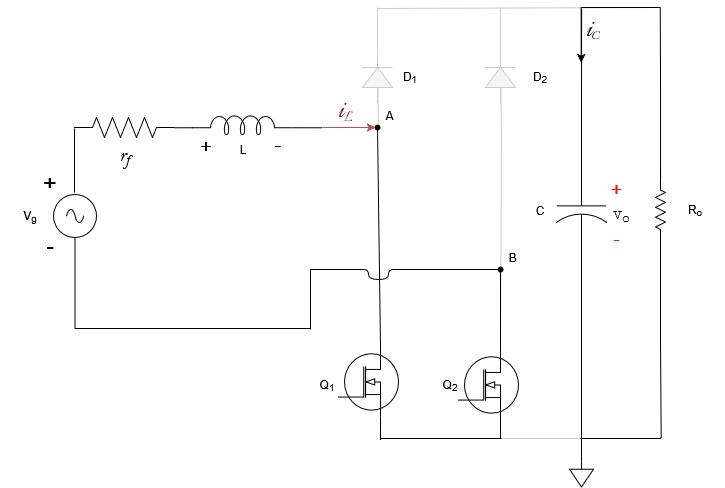
\includegraphics[width=\linewidth]{figures/circuit_1.png}
    \caption{Mode 1}
    \label{fig:mode1}
\end{figure}

\subsection{Operating Mode 1 (Charging)}

During operating mode 1, the input voltage $v_g(t)$ is positive, and both the switch devices, $Q_1$ and $Q_2$, are on. If we denote with $v_A$ the voltage potential at node $A$, and with $v_B$ the voltage potential at node $B$, we can write the following:

\begin{subequations}\begin{align}
    v_A = 0V \\
    v_B = 0V
\end{align}\end{subequations}

In other words, $Q_1$ and $Q_2$ pull the voltage potential at nodes $A$ and $B$ to ground, and thus $D_1$ and $D_2$ are reverse-biased.

\subsubsection*{KVL and KCL}
\begin{subequations}\begin{align}
    L\frac{di_L(t)}{dt} &= v_g(t) - r_fi_L(t) \\
    C\frac{dv_c(t)}{dt} &= -\frac{v_c(t)}{R_o}
\end{align}\end{subequations}

\begin{figure}[h]
    \centering
    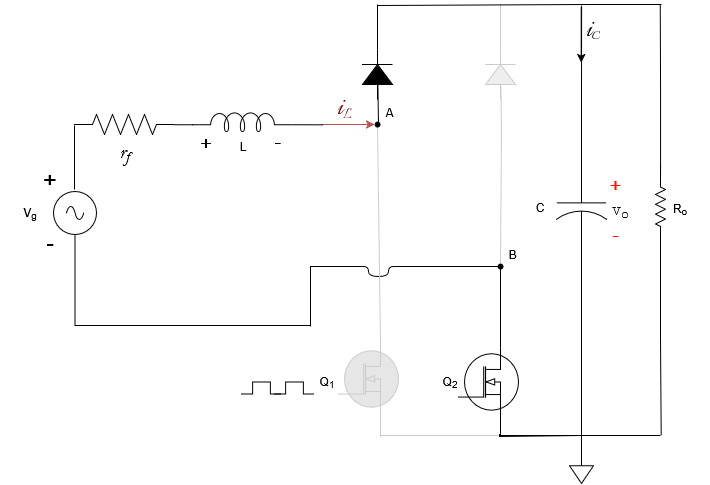
\includegraphics[width=\linewidth]{figures/circuit_2.png}
    \caption{Mode 2}
    \label{fig:mode2}
\end{figure}

\subsection{Operating Mode 2 (Loading the Output)}

In operating mode 2, the input voltage $v_g(t)$ is positive, and only the switch device $Q_2$ is on. 

\subsubsection*{KVL and KCL}
\begin{subequations}\begin{align}
    L\frac{di_L(t)}{dt} &= v_g(t) - r_fi_L(t)  - v_c(t)\\
    C\frac{dv_c(t)}{dt} &= i_L(t) - \frac{v_c(t)}{R_o}
\end{align}\end{subequations}
When $Q_1$ turns off, to push current forward, the inductor flips its internal voltage polarity. We can write:
\begin{subequations}\begin{align}
    v_A &= v_g(t) - v_L(t) - r_fi_L(t) \\
    v_B &= 0V
\end{align}\end{subequations}

where $v_L(t)$ denotes the d.o.p on the inductor $L$.

Thus, substituting the expression of $v_L(t)$ in $v_A$, we get that the voltage across $D_1$ is equal to:
\begin{align}
    v_{D_1} \simeq v_g(t) - v_L(t) - v_c(t) 
\end{align}

Therefore, $D_1$ is forward biased, while $D_2$ remains reverse biased. Nevertheless, there are some implicit assumptions to these results. As an example, consider when the input voltage crosses zero. In the limit case, when the inductor is incorrectly dimensioned, the system could enter \textit{Discontinuous Conduction Mode (DCM)}. Thus, we assume that $D_1$  behaves as a perfectly ideal component, and that the converter is designed to strictly maintain \textit{Continuous Conduction Mode (CCM)}. In other words, we assume that the inductor always possesses just enough energy to successfully force the diode in forward bias mode, keeping the equations valid across the entire AC cycle.

\begin{figure}[h]
    \centering
    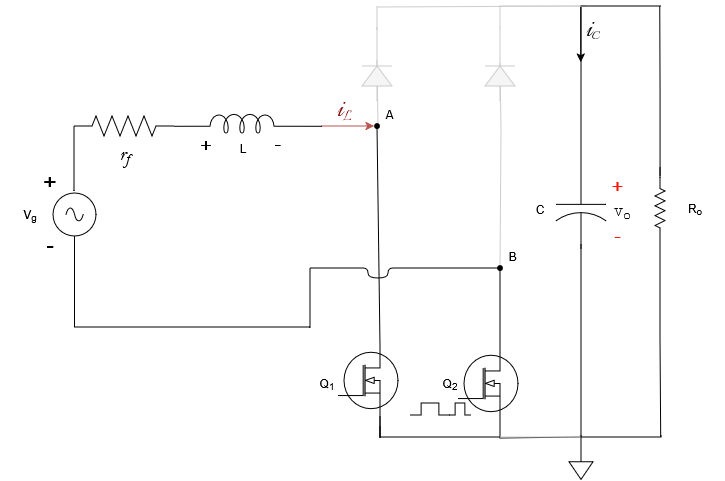
\includegraphics[width=\linewidth]{figures/circuit_3.png}
    \caption{Mode 3}
    \label{fig:mode3}
\end{figure}

\subsection{Operating Mode 3 (Reverse Charging)}
In operating mode 3, the input voltage is negative, and both switch devices $Q_1$ and $Q_2$ are on. 
As we noted during operating mode 1, since the switch devices pull the voltage potential at nodes $A$ and $B$ to ground, we can write:
\begin{subequations}\begin{align}
    v_A = 0V \\
    v_B = 0V
\end{align}\end{subequations}
Therefore, both $D_1$ and $D_2$ are reversed biased.
\subsubsection*{KVL and KCL}
\begin{subequations}\begin{align}
    L\frac{di_L(t)}{dt} &= v_g(t) - r_fi_L(t) \\
    C\frac{dv_c(t)}{dt} &= -\frac{v_c(t)}{R_o}
\end{align}\end{subequations}

\begin{figure}[h]
    \centering
    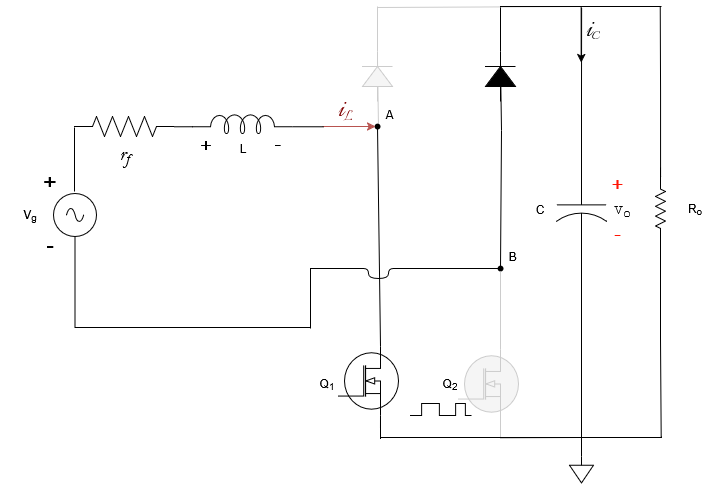
\includegraphics[width=\linewidth]{figures/circuit_4.png}
    \caption{Mode 4}
    \label{fig:mode4}
\end{figure}
\subsection{Operating Mode 4 (Loading the Output)}

In operating mode 4, the input voltage $v_g(t)$ is negative, and only the switch device $Q_1$ is on.

\subsubsection*{KVL and KCL}
\begin{subequations}\begin{align}
    L\frac{di_L(t)}{dt} &= v_g(t) - r_fi_L(t) + v_c(t) \\
    C\frac{dv_c(t)}{dt} &= -i_L(t) - \frac{v_c(t)}{R_o}
\end{align}\end{subequations}

When $Q_2$ turns off, to push current forward, the inductor flips its internal voltage polarity. Similarly to what we wrote during operating mode 2, we have:
\begin{subequations}\begin{align}
    v_A &= 0V \\
    v_B &= r_fi_L(t)+ v_L(t) - v_g(t)
\end{align}\end{subequations}

Substituting the expression of $v_L(t)$ in $v_B$, we can write:

\begin{align}
    v_{D_2} \simeq v_L(t) - v_g(t) - v_c(t) 
\end{align}

Therefore, $D_2$ is forward biased, while $D_1$ remains reverse biased.
%------------------------------------------------

\section {Switched Model}
Defining $\delta_1(t)$ as the modulating switching function and $\delta_2(t)$ as the polarity function of the input voltage $v_g(t)$, we obtain:
\[
\delta_1(t) = \begin{cases} 
1, & 0 < t \le \tau_{ON} \\ 
0, & \tau_{ON} < t < T 
\end{cases}
\]

\[
\delta_2(t) = \begin{cases} 
1, & v_g(t) > 0 \\ 
0, & v_g(t) < 0 
\end{cases}
\]
{\small
\begin{equation}
\begin{aligned}
L \frac{di_L}{dt} &= \delta_2 \left[ (v_g - r_f i_L)\delta_1 + (v_g - r_f i_L - v_c)(1 - \delta_1) \right] + \\
&\quad + [1 - \delta_2][(v_g - r_f i_L)\delta_1 + \\
&\quad + (v_g + v_c - r_f i_L)(1 - \delta_1)] \\[10pt]
% &= (v_g - r_f i_L) \big[ \delta_2\delta_1 + \delta_2(1 - \delta_1) + \\
% &\quad + \delta_1(1 - \delta_2) + (1 - \delta_1)(1 - \delta_2) \big] - \\
% &\quad - \delta_2V_c(1 - \delta_1) + V_c(1 - \delta_2)(1 - \delta_1) \\[10pt]
&= (v_g - r_f i_L) + v_c(1 - \delta_1)(1 - 2\delta_2)
\end{aligned}
\end{equation}
}
%\vspace{1em}
Considering $v_g(t)>0$, the term $(1 - 2\delta_2(t))$, becomes equal to $-1$, instead, considering $v_g(t)<0$ the same term becomes equal to $1$. So, it is possible to introduce $\text{sgn}(v_g(t))$ to include all various cases:

\begin{equation}
	-\text{sgn}(v_g) = (1 - 2\delta_2) = 
\begin{cases}
    -1, \quad \delta_2 = 1 \\
     1, \quad \delta_2 = 0
\end{cases}
\end{equation}
In conclusion we obtain:
\begin{equation}
L \frac{di_L(t)}{dt} = (v_g(t) - r_f i_L(t)) - v_c(t) (1 - \delta_1(t)) \text{sgn}(v_g(t))
\end{equation}

Applying the same strategy to the second state-equation, we obtain:
\begin{equation}
\begin{aligned}
C \frac{dv_c(t)}{dt} &= -\frac{v_c(t)}{R_o} + i_L(t) (1 - \delta_1(t)) \operatorname{sgn}(v_g(t))
\end{aligned}
\end{equation}

The final system of the state-equation, describing  all the four operating modes, is:
{\small
\begin{equation}
\begin{cases} 
L \frac{di_L(t)}{dt} = v_g(t) - r_f i_L(t) - (1 - \delta_1(t)) v_c(t) \operatorname{sgn}(v_g(t)) \\ 
C \frac{dv_c(t)}{dt} = -\frac{v_c(t)}{R_o} + (1 - \delta_1(t)) i_L(t) \operatorname{sgn}(v_g(t)) 
\end{cases}
\end{equation}
}
The system state variables are defined as:
\begin{equation}
x(t) = \begin{bmatrix}i_L(t) \\ v_c(t) \end{bmatrix}
\end{equation}


For $\delta_1(t)=1$ the system becomes:
\begin{equation}
\dot{x}(t) = \underbrace{\begin{bmatrix} -\frac{r_f}{L} & 0 \\ 0 & -\frac{1}{R_o C} \end{bmatrix}}_{A_1} x(t) + \underbrace{\begin{bmatrix} \frac{1}{L} \\ 0 \end{bmatrix}}_{B_1} v_g(t)
\end{equation}

For $\delta_1(t)=0$, the system is described as:
\begin{equation}
\dot{x}(t) = \underbrace{\begin{bmatrix} 
-\frac{r_f}{L} & -\frac{\operatorname{sgn}(v_g(t))}{L} \\ 
\frac{\operatorname{sgn}(v_g(t))}{C} & -\frac{1}{R_o C} 
\end{bmatrix}}_{A_0(t)} x(t) + 
\underbrace{\begin{bmatrix} 
\frac{1}{L} \\ 
0 
\end{bmatrix}}_{B_0} v_g(t)
\end{equation}

In conclusion, the equation that describes the switched model of the entire system is given by:
\begin{align*}
\dot{x}(t) = (A_1 x(t) &+ B_1 v_g(t))\delta_1(t) + \\ &+ (A_0(t) x(t) + B_0 v_g(t))(1 - \delta_1(t))
\end{align*}

This system becomes a system that switches between two modes, one of which is time-variant.

\section{Averaged Model}
The averaged model replicates the average behavior of the power converter and it can be obtained based on switched model.

\begin{equation}
\dot{\bar{x}}(t) = (A_1 - A_0(t))\bar{x}(t) d(t) + A_0(t) \bar{x}(t) + B_0 \bar{v}_g(t)
\end{equation}

where $d(t)$ and $\bar{x}(t)$ are respectively the duty cycle of the system and the mean value of the state-variable, obtained applying time averaging over a switching period $T_s$.
\begin{equation}
\begin{aligned}
\langle \delta_1(t) \rangle_{T_s} = \frac{1}{T_s} \int_{t - \frac{T_s}{2}}^{t + \frac{T_s}{2}} \delta_1(\tau) \, d\tau = \frac{1}{T_s} \int_{0}^{\tau_{on}} 1 \, d\tau = \\=\frac{\tau_{on}}{T_s} = d(t)
\end{aligned}
\end{equation}
\begin{equation}
\langle x(t) \rangle_{T_s} = \frac{1}{T_s} \int_{t - \frac{T_s}{2}}^{t + \frac{T_s}{2}} x(\tau) \, d\tau
\end{equation}
Assuming that the sign of the voltage $v_g(t)$ changes very slowly with respect to the switching frequency, we can consider the function $sgn(v_g(t))$ constant in $T_s$.
It is possible to write the averaged model as:
{\small
\begin{equation}\label{averaged_model}
\begin{cases} 
\dfrac{d \bar{i}_L(t)}{dt} = \dfrac{-r_f \bar{i}_L(t) - \operatorname{sgn}(v_g(t))(1-d(t))\bar{v}_c(t) + \bar{v}_g(t)}{L} \\[20pt]
\dfrac{d \bar{v}_c(t)}{dt} = \dfrac{R_o \operatorname{sgn}(v_g(t))(1-d(t)) \bar{i}_L(t) - \bar{v}_c(t)}{R_oC} 
\end{cases}
\end{equation}
}
Equivalently, in matrix form, we have:
\begin{gather}
\dot{\bar{x}}(t) = \begin{bmatrix} 0 & \frac{\operatorname{sgn}(v_g(t))}{L} \\ -\frac{\operatorname{sgn}(v_g(t))}{C} & 0 \end{bmatrix} \bar{x}(t) d(t) + \\ \begin{bmatrix} -\frac{r_f}{L} & -\frac{\operatorname{sgn}(v_g(t))}{L} \\ \frac{\operatorname{sgn}(v_g(t))}{C} & -\frac{1}{R_o C} \end{bmatrix} \bar{x}(t)
+\begin{bmatrix} \frac{1}{L} \\ 0 \end{bmatrix} v_g(t) 
\end{gather}

Thus, we have:
{\small
\begin{equation}
    \dot{\bar{x}}(t)= \begin{bmatrix} -\frac{r_f}{L} & -\frac{(1-d(t))\operatorname{sgn}(v_g(t))}{L} \\[6pt] \frac{(1-d(t))\operatorname{sgn}(v_g(t))}{C} & -\frac{1}{R_o C} \end{bmatrix} \bar{x}(t) + \begin{bmatrix} \frac{1}{L} \\ 0 \end{bmatrix} v_g(t) 
\end{equation}
}

\section{Small signal analysis}
\subsection{Operating Trajectory}
The Bridgeless Boost PFC Converter has $v_g(t)$ as a sinusoidal forcing. The state variable  $i_L(t)$ gets to be sinusoidal and with the same phase as $v_g(t)$ in order to get PFC. The output voltage and $v_c(t)$ become constant due to the rectifier effect. Since the period of the grid voltage is slow with respect to the period of the average operation, we can approximate the average of $i_L(t)$, $v_g(t)$ and  $v_c(t)$ with their actual expression.
We rewrite the system control variable to be the following:
\begin{equation}
u(t)=d(t)
\end{equation}

This condition gives the trajectory of the state:
\begin{equation}
\begin{cases}
% $$\bar{V}_{g_{tj}}$$ (t) = V_{in} sin($$\omega$$t) = v_g(t)\\
$$\bar{i}_{L_{tj}}$$ (t) = I_L \sin($$\omega$$t) = i^*_L(t)\\
$$\bar{v}_{c_{tj}(t)}$$ = V^*_{o } \Rightarrow \dfrac{d \bar{v}_{c_{tj}}(t)}{dt} = 0
\end{cases}
\end{equation}
Applying the trajectory of the states and the forcement the system at steady-state can be written like:
{\small
\begin{equation}\label{eq:steady-state}
\begin{cases} 
\dfrac{d i^*_L(t)}{dt} = \dfrac{-r_f i^*_L(t) - \operatorname{sgn}(v_g(t)) ( 1- u_o(t)) V^*_{o} + v_g(t)}{L} \\[16pt]
0 = \dfrac{R_o ( 1- u_o(t))|i^*_L(t)| - V^*_{o}}{R_oC} \\[16pt]

\end{cases}
\end{equation}
}
where we have used $\text{sgn}(v_g(t)) i^*_L(t) = |i^*_L(t)|$ since $v_g(t)$ is sinusoidal and in phase with $i^*_L(t)$. Therefore, the product $\operatorname{sgn}(v_g(t))i^*_L(t)$ will always be positive and have the same amplitude as $i^*_L(t)$.
% Multiplying on both sides by $\text{sgn}(v_g(t))$, we can write the KVL at steady-state as:
% \begin{equation}
% \dfrac{d |i^*_L|}{dt} = \dfrac{-r_f |i^*_L| - ( 1- u_o(t)) V^*_{o} + |v_g(t)|}{L} \\[16pt]
% \end{equation}

% where we have used $\text{sgn}(v_g(t))\dfrac{d i^*_L}{dt} = \dfrac{d |i^*_L|}{dt}$.
From the second equation in (\ref{eq:steady-state}), we can obtain $u_o(t)$ as follows:

{\small
\begin{equation} \label{eq:steady_state_control}
u_o(t)= \dfrac{1}{|i^*_L(t)|}(|i^*_L(t)|- \dfrac{V^*_{o}}{R_o})
\end{equation}
}


Substituting this value in the first equation in (\ref{eq:steady-state}), and using the following trigonometrical expression:

\begin{equation}\label{eq:sin2wt}
\sin^2(\omega t) = \dfrac{1-\cos(2\omega t)}{2}
\end{equation}

\begin{equation}\label{eq:cossin}
\cos(\omega t)\sin(\omega t) = \dfrac{\sin(2\omega t)}{2}
\end{equation}

we get the following relation:

{\small
\begin{equation}\label{eq:active_power_balance}
\begin{split}
\quad \omega L I_L^2 \frac{1}{2} \sin(2\omega t) = (V_g I_L&-r_f I_L^2 ) \dfrac{1-\cos(2\omega t)}{2} - \\ - \frac{(V_0^*)^2}{R_0} 
\end{split}
\end{equation}
}

Averaging over the fundamental period $T=\dfrac{2\pi}{\omega}$ Eq. (\ref{eq:active_power_balance}), we will get the following expression:

{\small
\begin{equation}\label{eq:avrage_power_balance}
\begin{split}
\quad \omega L I_L^2\frac{1}{T}\int_{0}^T{\frac{1}{2} \sin(2\omega t) dt}=\\
= (V_g I_L-r_f I_L^2 ) \frac{1}{T}\int_{0}^T{\dfrac{1-\cos(2\omega t)}{2} dt}- &\\ - \frac{(V_0^*)^2}{R_0} \frac{1}{T}\int_{0}^T{dt}
\end{split}
\end{equation}
}

Solving the integrals in (\ref{eq:avrage_power_balance}), yields:


\begin{equation}\label{eq:integral sin}
\frac{1}{T}\int_{0}^{T} \frac{1}{2} \sin(2\omega t) \, dt = \frac{1}{T}\left[ -\frac{1}{4\omega} \cos(2\omega t) \right]_{0}^{T}= 0
\end{equation}

\begin{equation}\label{eq:integral cos}
\frac{1}{T}\int_{0}^T{\dfrac{1-\cos(2\omega t)}{2} dt} = \frac{1}{T}\left[ t -\frac{1}{4\omega} \sin(2\omega t) \right]_{0}^{T}= \frac{1}{2}
\end{equation}

Thus, Eq. (\ref{eq:avrage_power_balance}) can be rewrite like following:

\begin{align}\label{eq:power_balance}
 \underbrace{\dfrac{1}{2}V_g I_L}_{P_{in}} - \underbrace{\dfrac{1}{2}r_f I_L^2}_{P_{loss}} - \underbrace{\dfrac{(V^*_{o})^2 }{R_o}}_{P_{out}} = 0 
\end{align}

Eq. (\ref{eq:power_balance}) represents the active power balance of the system and is, by definition, equal to zero. This shows that choosing the control variable like $u_o(t)$ keeps $v_c(t)$ equal, on average, to the reference value. 
From Eq. (\ref{eq:power_balance}), we can calculate the peak of the sinusoidal current to use for the trajectory like following:

\begin{align} \label{eq:peak_current}
I_L= \dfrac{1}{2}\dfrac{V_g}{r_f}\left(1-\sqrt{1-8\dfrac{{V^*_{o}}^2}{V_g^2}\dfrac{r_f}{R_o}}\right)
\end{align}

Assuming real solutions, solving Eq. (\ref{eq:peak_current}), we chose the smaller solution to limit the current that is drained from the grid and limit the dissipation of power in the resistor $r_f$.

\subsection{Linearized State-Space Model}
In order to linearize the system, we can consider the variation of the variable of the system with respect to its working point. The working point of the system is time varying, and it depends on the trajectory. So we are considering variations around the trajectory. These can be expressed as:
\begin{equation}
\begin{cases}
\Delta{u}(t) = u(t) - u_o(t)\\
\Delta{x}(t) = \bar{x}(t) - x_{tj}(t) \\
\Delta{v}_g(t) = \bar{v}_g(t) - v_g(t)
\end{cases}
\end{equation}
where $x_{tj}(t)$, $v_g(t)$ and $u_o$ are the values of the trajectory.
Linear control laws can be obtained based on the linearization of the model around the trajectory imposed and calculated in the previous section.\\ 
The linearized system can be written like:
\begin{equation}
\begin{split}
\dot{\bar{x}} = f(\bar{x}(t), u(t), \bar{v}_g(t))|_{x_{tj},u_o, v_g} +  \left. \frac{\partial f}{\partial \bar{x}} \right|_{x_{tj},u_o, v_g} \Delta{x}(t) \\ + \left. \frac{\partial f}{\partial u} \right|_{x_{tj}, u_o, v_g} \Delta{u}(t) + \left. \frac{\partial f}{\partial \bar{v}_g} \right|_{x_{tj}, u_o(t), v_g} \Delta{v_g(t)}
\end{split}
\end{equation}
\\Applying the derivative and writing the state-space model in matrix form, we obtain:
{\small
\begin{equation}
\frac{d}{dt}(\bar{x} - x_{tj}) = \frac{d\bar{x}}{dt} - {\frac{dx_{tj}}{dt}} = \dot{\bar{x}} - \dot{x}_{tj} = \\\Delta{\dot{x}}
\end{equation}
}
where $\dot{x}_{tj} = f(\bar{x}, u, \bar{v}_g)|_{x_{tj},u_o, v_g}$, and time dependency has been omitted for simplicity.

The linearized model can be written as:

\begin{comment}
\begin{equation}
\dot{\tilde{x}} = (A_1 D + A_0 D') \tilde{x} + (A_1 - A_0) x_{eq} \tilde{d} + B_0 \tilde{V}_g
\end{equation}
\end{comment}

{\small
\begin{equation}
\begin{split}
\dot{\bar{x}} &=
\underbrace{
\begin{bmatrix} 
\dfrac{-r_f |i^*_L| - ( 1- u_o) V^*_{o} + |v_g|}{L}\\[12pt] 
\dfrac{R_o ( 1- u_o)|i^*_L| - V^*_{o}}{R_oC}
\end{bmatrix}}_{\dot{x}_{tj}(t)} \\
&\quad +
\underbrace{
\begin{bmatrix} 
-\dfrac{r_f}{L} & -\dfrac{\operatorname{sgn}(v_g) ( 1- u_o)}{L} \\[12pt] 
\dfrac{\operatorname{sgn}(v_g) ( 1- u_o)}{C} & -\dfrac{1}{R_o C} 
\end{bmatrix}}_{A(t)} \Delta{x} \\
&\quad + 
\underbrace{
\begin{bmatrix} 
\dfrac{V^*_{o} \text{sgn}(v_g)}{L} \\[12pt] 
-\dfrac{|i^*_{L}|}{C} 
\end{bmatrix}}_{B_d(t)} \Delta{u} + 
\underbrace{
\begin{bmatrix} 
\dfrac{1}{L} \\[8pt] 
0 
\end{bmatrix}}_{B_v} \Delta{v}_g
\end{split}
\end{equation}
}

where time dependency has been omitted for simplicity.
Bringing the term $\dot{x}_{tj}(t)$ on the LHS we have the following small-signal model:

{\small
\begin{equation}
\begin{split}
\Delta{\dot{x}} &=
\underbrace{
\begin{bmatrix} 
-\dfrac{r_f}{L} & -\dfrac{\operatorname{sgn}(v_g) ( 1- u_o)}{L} \\[12pt] 
\dfrac{\operatorname{sgn}(v_g) ( 1- u_o)}{C} & -\dfrac{1}{R_o C} 
\end{bmatrix}}_{A(t)} \Delta{x} \\
&\quad + 
\underbrace{
\begin{bmatrix} 
\dfrac{V^*_{o} \text{sgn}(v_g)}{L} \\[12pt] 
-\dfrac{|i^*_{L}|}{C} 
\end{bmatrix}}_{B_d(t)} \Delta{u} + 
\underbrace{
\begin{bmatrix} 
\dfrac{1}{L} \\[8pt] 
0 
\end{bmatrix}}_{B_v} \Delta{v}_g
\end{split}
\end{equation}
}
% In getting the linearized model, we assumed that the derivative of sgn($(v_g(t)$) is always equal to zero, considering sgn($v_g(t)$) always constant. With this assumption, we neglect the Dirac impulse when $v_g(t)$ crosses zero.
% The linearized model is a time variant system since the dynamic equation and the input equation are time-dependent.

% \section{S-domain Model}
% The Bridgeless Boost PFC Converter transfer functions can be derived from the linearized state-space small-signal model. To do that, since the system dynamics change with time, we can write the transfer function at a specific time instant when $\theta = \omega t =\dfrac{\pi}{2}+ 2k\pi$ where $k\in 
% \mathbb{Z}$.
% Since the dynamic and control matrices change slowly (frequency of the voltage grid) relative to the system dynamics, we can analyze the transfer function at each time instant. If the system is stable in each time instant, we can use the worst-case transfer function to project the system control.
% Since when the grid voltage is positive, and at peak we have a positive zero, this is the worst case for the control design. The poles of the system are the same for the positive and negative semiperiod.
% Therefore, even if the transfer functions are time-varying, we proceed to consider the transfer functions for the worst case.\\

% With this assumption, we can write the following:
% \begin{align}
% v_g(t) &= V_g \\
% \operatorname{sgn}(v_g(t))&=1 \\
% u_o(t) &= D\\
% D'&=1-D\\
% \Delta{d} &= d - D
% \end{align}
% These conditions allow to write $A(t) = A$ and $B_d(t) = B_d$, which yields the following:
% {\small
% \begin{equation}
% \Delta{X}(s) = (sI - A)^{-1} B_d \Delta{d}(s) + (sI - A)^{-1} B_v \Delta{V}_g(s)
% \end{equation}
% }
% where $(sI-A)^{-1}$ and $\Delta(s)$ are expressed as:
% {\small
% \begin{equation}
% \begin{aligned}
% (sI - A)^{-1} &= \frac{1}{\Delta(s)}
% \begin{pmatrix} 
% s + \dfrac{1}{R_0 C} & -\dfrac{D'}{L} \\[12pt] 
% \dfrac{D'}{C} & s + \dfrac{r_f}{L} 
% \end{pmatrix} \\[20pt]
% \Delta(s) &= s^2 + s \left[ \frac{r_f R_0 C + L}{R_0 L C} \right] + \frac{(D')^2 R_0 + r_f}{R_0 L C}
% \end{aligned}
% \end{equation}
% }

% {\small
% Below are reported all the transfer functions that describe the entire system:
% \begin{equation}\label{eq:Control-to-Output Voltaage Transfer Function}
% G_{vd}(s) = \frac{\dfrac{\mathrm{V_g} R_0}{(R_0 (D')^2 + r_f)^2} \Big[ R_0 (D')^2 - r_f - sL \Big]}{\dfrac{R_0 LC}{(D')^2 R_0 + r_f} s^2 + s \left( \dfrac{r_f R_0 C + L}{(D')^2 R_0 + r_f} \right) + 1}
% \end{equation}
% }
% It is possible to rewrite the Control-to-Output Voltage Transfer Function Eq. (\ref{eq:Control-to-Output Voltaage Transfer Function}), in terms of the gain $K_{vd}$, the damping factor $\zeta$,  the natural pulsation $\omega_n$ and the RPH (Right Half Plane) $\omega_z$ (or in other words the so called non minimum phase zero that corresponds to a system whose response to an input exhibits non-monotonic behavior, often characterized by an initial response in the opposite direction of the intended output).

% \begin{equation}
% G_{vd}(s) = K_{vd} \frac{\left( 1 - \frac{s}{\omega_z} \right)}{\frac{s^2}{\omega_n^2} + \frac{2\zeta s}{\omega_n} + 1}
% \end{equation}

% \begin{equation}
% \omega_z = \frac{R_0 (D')^2 - r_f}{L}
% \end{equation}

% \begin{equation}
% K_{vd} = \frac{\mathrm{V_g} R_0}{(R_0 (D')^2 + r_f)^2} \left[ R_0 (D')^2 - r_f \right]
% \end{equation}

% \begin{equation}
% \omega_n = \sqrt{\frac{(D')^2 R_0 + r_f}{R_0 L C}}
% \end{equation}

% {\small
% \begin{equation}
% \begin{split}
% \zeta &= \frac{1}{2} \frac{r_f R_0 C + L}{(D')^2 R_0 + r_f} \sqrt{\frac{(D')^2 R_0 + r_f}{R_0 L C}} = \\
%       &= \frac{1}{2\omega_n} \left( \frac{r_f}{L} + \frac{1}{R_0 C} \right)
% \end{split}
% \end{equation}
% }
% The same strategy is applied to the Control-to-Inductor Current Transfer Function:

% {\small
% \begin{equation}
% G_{id}(s) = \frac{\dfrac{2\mathrm{V_g} D' R_0}{((D')^2 R_0 + r_f)^2} \left( \dfrac{s R_0 C}{2} + 1 \right)}{\dfrac{R_0 L C}{(D')^2 R_0 + r_f} s^2 + s \left( \dfrac{r_f R_0 C + L}{(D')^2 R_0 + r_f} \right) + 1}
% \end{equation}

% \begin{equation}
% G_{id}(s) = K_{id} \frac{\left( 1 + \dfrac{s}{\omega_z} \right)}{\dfrac{s^2}{\omega_n^2} + s \dfrac{2\zeta}{\omega_n} + 1}
% \end{equation}

% \begin{equation}
% K_{id} = \frac{2 \mathrm{V_g} D' R_0}{((D')^2 R_0 + r_f)^2}
% \end{equation}
% \begin{equation}
% \omega_z = \frac{2}{R_0 C}
% \end{equation}
% }


\section{Control Systems Analysis}
The first control strategy, Lyapunov-Based Control, constructs an energy-based Lyapunov candidate function that enforces a strictly negative time derivative. The synthesised control law guarantees global asymptotic stability and directly forces the time-varying tracking errors to zero.

The second control scheme, the Cascaded PI/PR Control strategy, uses a low-bandwidth outer PI loop to regulate the DC output voltage, and a fast inner Proportional-Resonant (PR) loop tracks the sinusoidal current reference.

Finally, the third approach, Dynamic Phasor Domain Control, utilizes orthogonal signal generation (SOGI) and synchronous reference frame transformations to map the time-varying AC variables into DC-equivalent active and reactive components. By applying an algebraic feedforward decoupling network, the system is linearized and cross-coupling is canceled, allowing standard PI controllers to operate on flat DC references with high bandwidth.

The following results in the S-domain are derived based on the system transfer functions defined in Appendix A. Indeed, it is important to note that, because we are dealing with a time-varying system, the PI/PR controllers are tuned based on the worst-case transfer functions, which correspond to the time instants when the input voltage is at its peak.
\subsection{Lyapunov-based Control Scheme}
In \cite{TU}, the authors propose a two-loop cascade control structure composed of an external and internal control loop. The Outer-Control loop is composed of a Proportional-Integral (PI) lineal controller, whose purpose is to generate the reference signal for the inductor current $i^*_L$, using the output voltage error signal to produce the instantaneous current reference. The inner-control loop, on the other hand, instead of being implemented with yet another PI controller, is based on the Lyapunov method for stability. Indeed, an error-system is defined, with the objective of determining the control $\Delta u$ that achieves asymptotic stability, thus achieving zero steady-state error. The overall control scheme is shown in Fig. \ref{fig:lyapunov}.
\subsubsection{Outer Voltage Loop}
\begin{figure*}[htp]
    \centering
    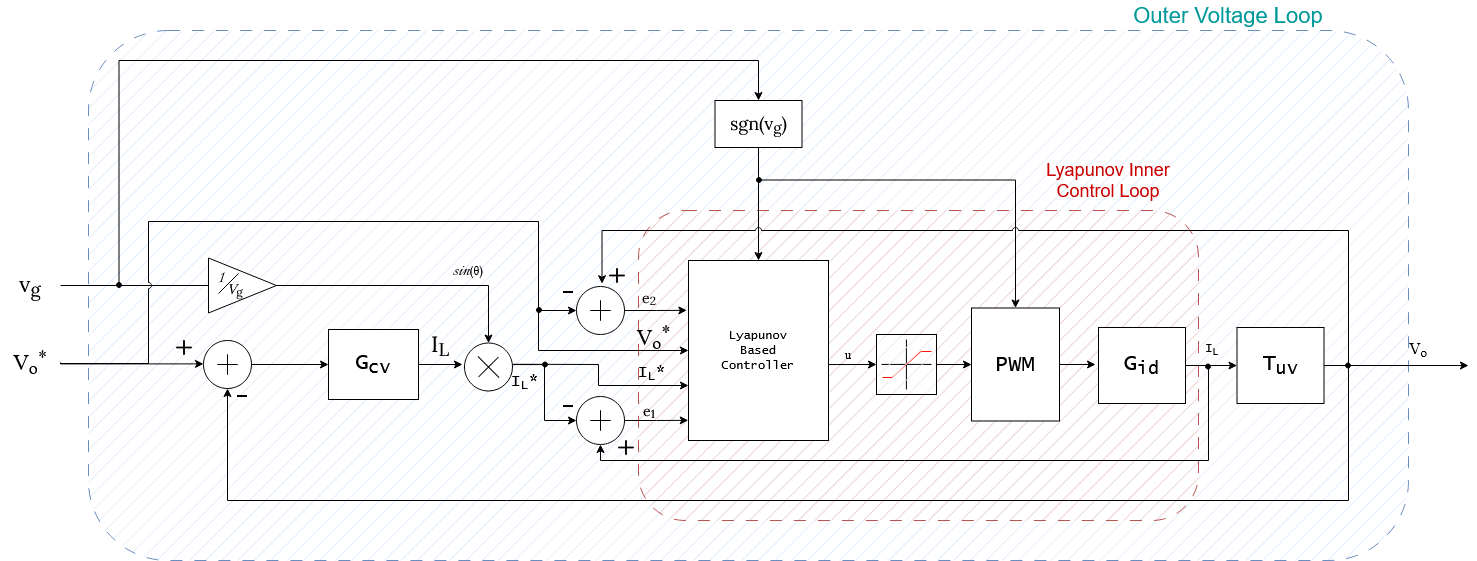
\includegraphics[width=0.8\linewidth]{figures/lyapunov.drawio(1).png}
    \caption{Lyapunov-based Control Scheme}
    \label{fig:lyapunov}
\end{figure*}
The outer voltage loop compensates for the voltage error. We define $G_{cv}(s)$ as the transfer function of the PI controller, whose bode plot is shown in Fig \ref{fig:bode_PI}:
\begin{equation}\label{eq:G_cv}
\begin{aligned}
G_{cv}(s) = K_p + \frac{K_i}{s} &= G_{m_{cv}} + \frac{G_{m_{cv}} \omega_z}{s} \\
&= \frac{G_{m_{cv}} s + G_{m_{cv}} \omega_z}{s} \\
&= G_{m_{cv}} \omega_z \frac{\left( 1 + \frac{s}{\omega_z} \right)}{s}
\end{aligned}
\end{equation}

\begin{figure}
    \centering
    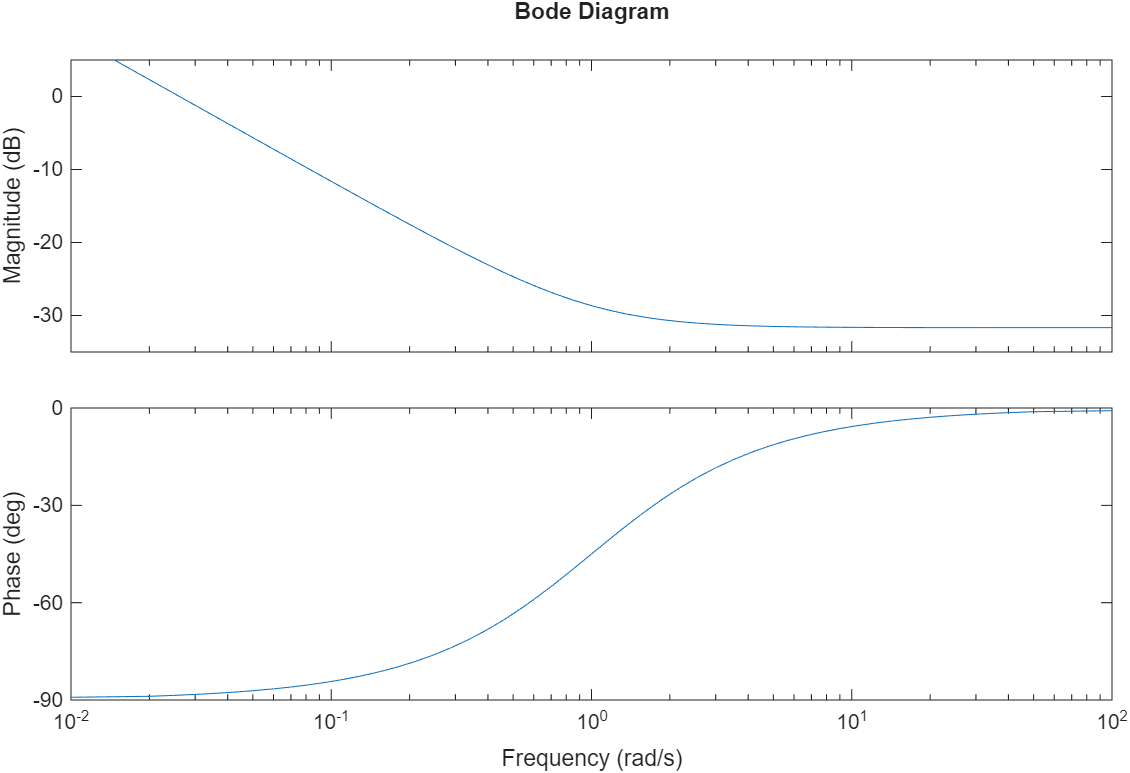
\includegraphics[width=\linewidth]{figures/bode_PI.png}
    \caption{Bode plot of $G_{cv}$}
    \label{fig:bode_PI}
\end{figure}
% \begin{equation}\label{eq:open_loop}
% \begin{aligned}
% L(s) &=G_{cv}(s) T_{uv}(s) =\\
% &=\left[ G_{m_{cv}} \omega_{z_{cv}} \frac{\left( 1 + \frac{s}{\omega_{z_{cv}}} \right)}{s} \right] T_{uv_0} \frac{\left( 1 - \frac{s}{\omega_z} \right)}{\left( 1 + \frac{s}{\omega_p} \right)}
% \end{aligned}
% \end{equation}
% }

The inductor current reference is then obtained as:
\begin{equation}\label{eq:reference_ind_curr}
    i^*_L = I_L \frac{v_g}{V_{g}}
\end{equation}
where $V_g$ is the peak of the input grid voltage $v_g(t)$.

%\begin{figure}
%	\centering
%	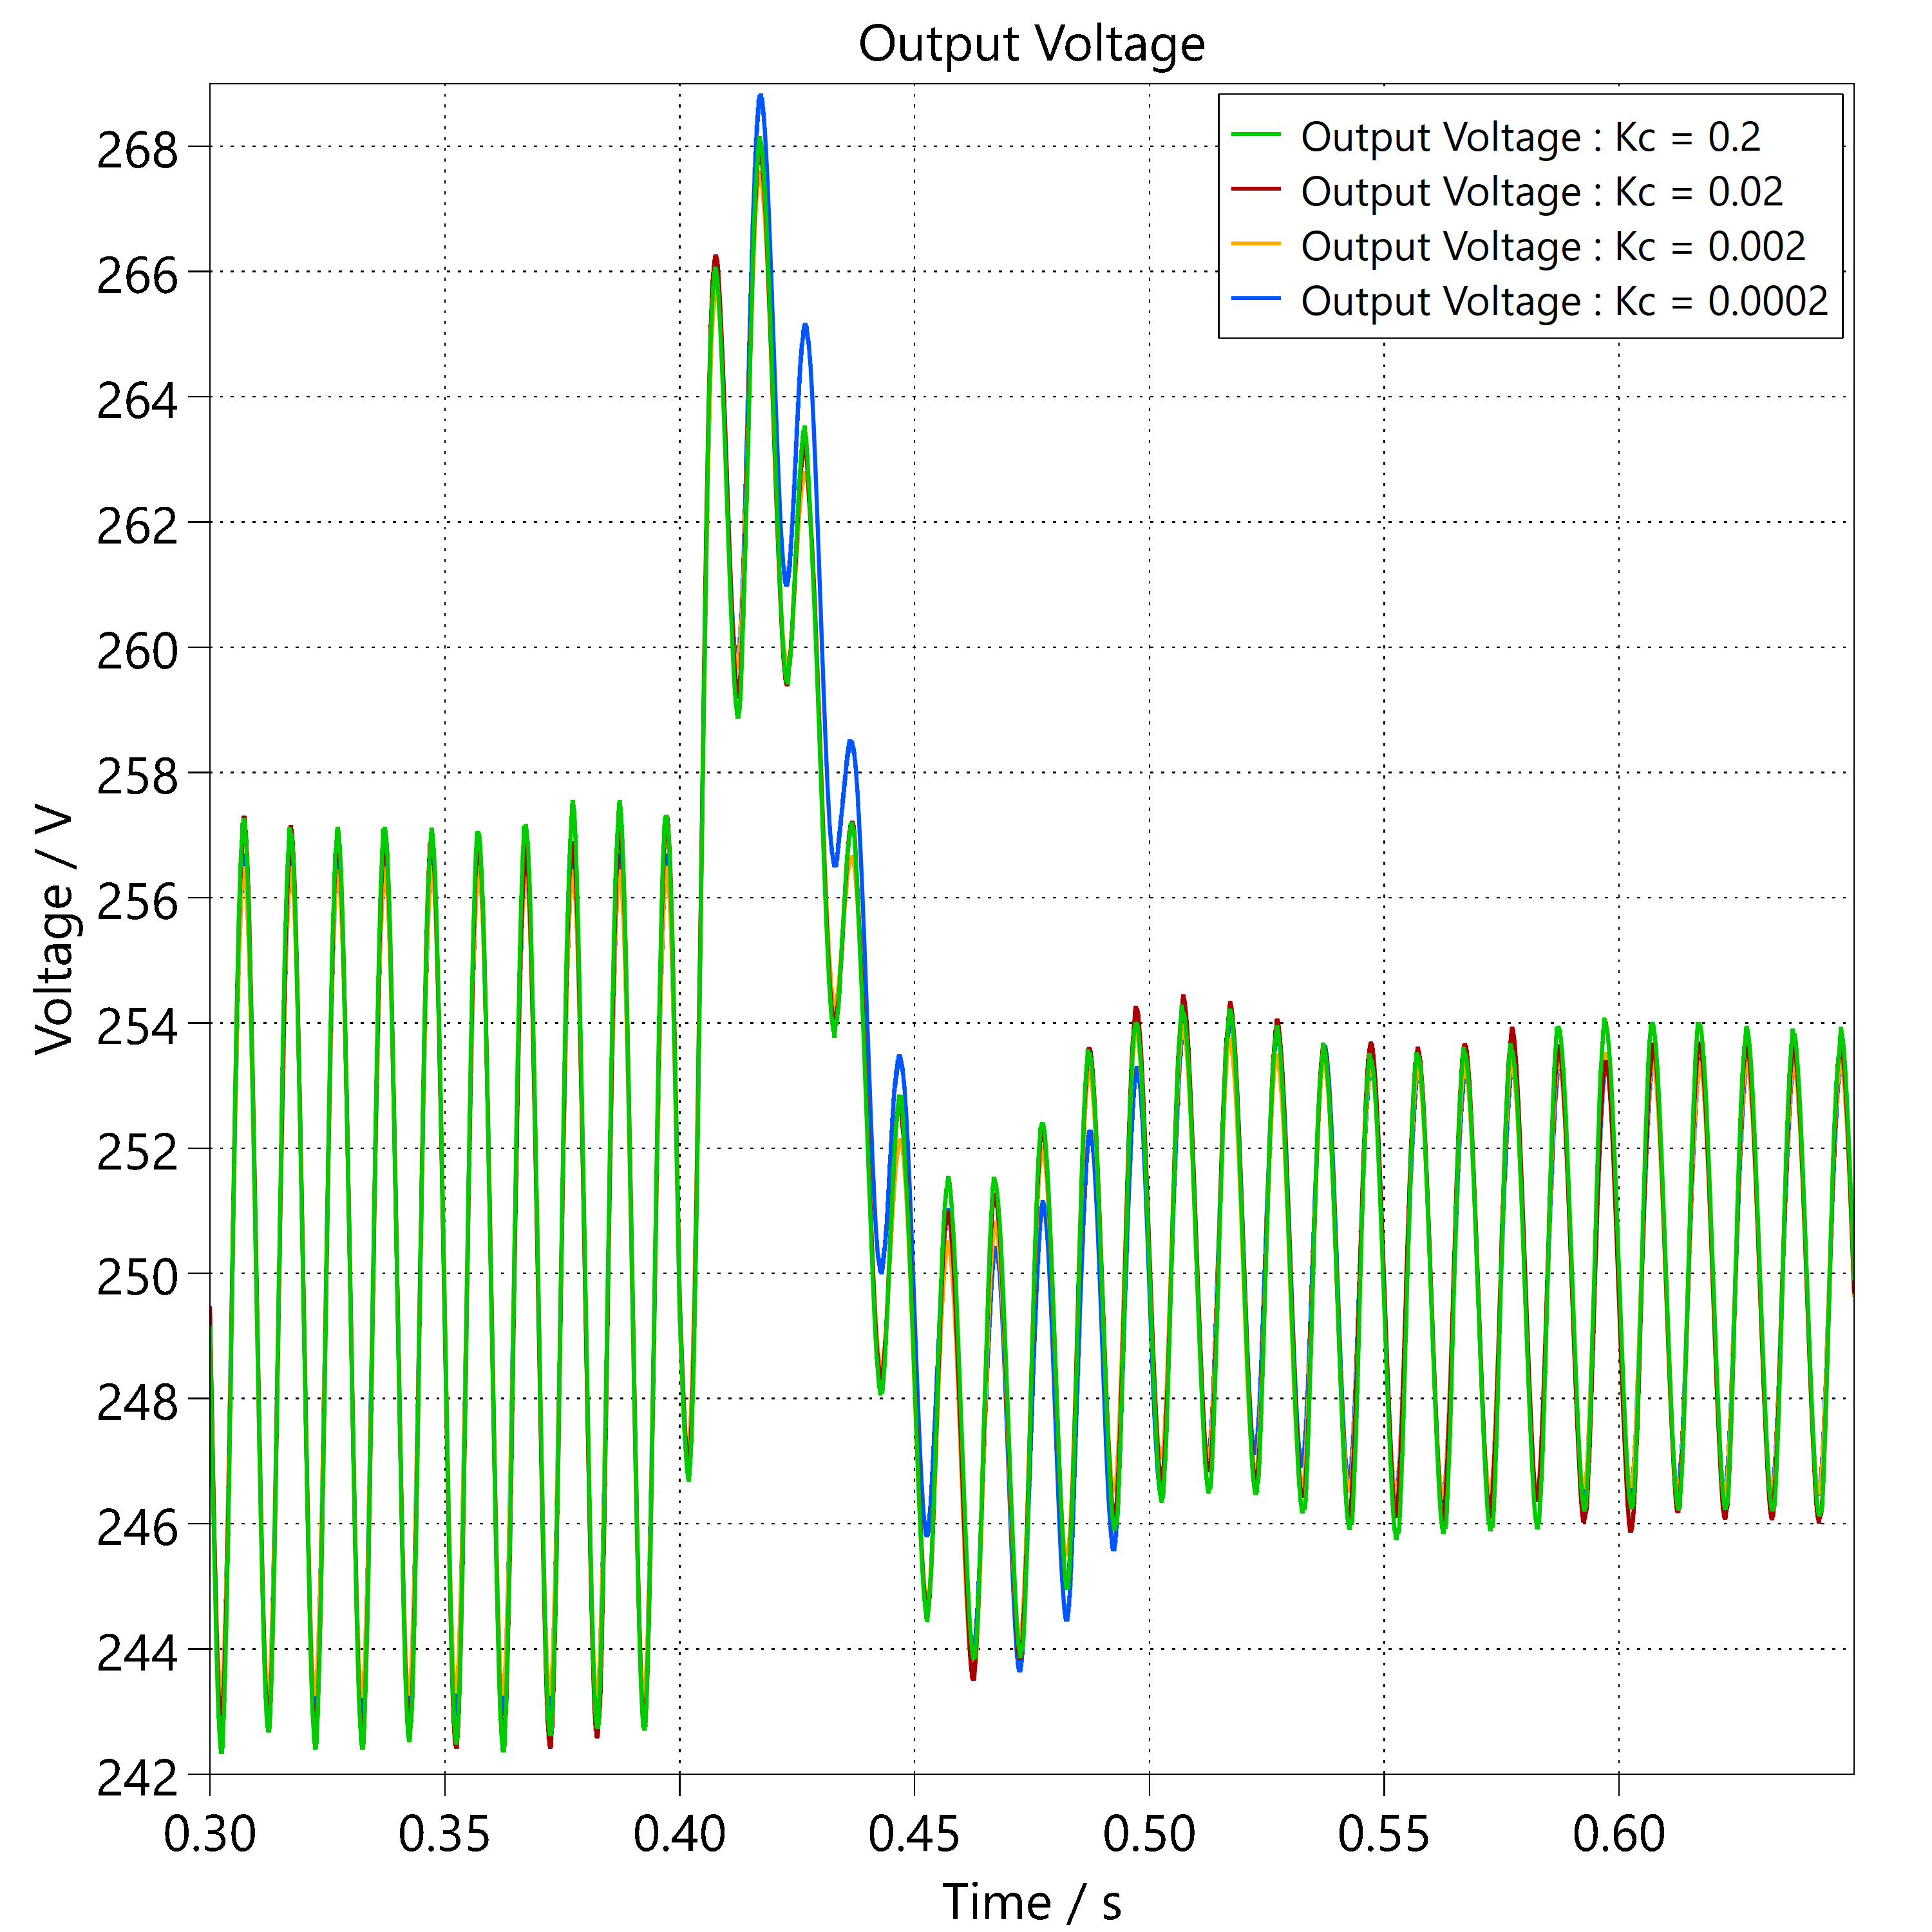
\includegraphics[width=0.7\linewidth]{figures/LY_vo_kc_paper}
%	\caption{}
%	\label{fig:lyvokcpaper}
%\end{figure}


\subsubsection{Inner Lyapunov Loop}
In the Lyapunov control method, an energy function that includes closed-loop dynamics must be defined to derive the appropriate control input.

First, we define the tracking error vector $e$. We want the actual inductor current $\bar{i}_L$ to track the reference $i_L^*$, and the actual capacitor voltage $\bar{v}_c$ to track the reference $V_0^*$. 
\begin{equation}\label{eq:error_state}
    e = \begin{bmatrix} e_1 \\ e_2 \end{bmatrix} \triangleq \begin{bmatrix} \bar{i}_L - i_L^* \\ \bar{v}_c - V_0^* \end{bmatrix}
\end{equation}

Next, we define an energy-based Lyapunov candidate function $V(e)$, which must be positive definite ($V(e) > 0$ for all $e \neq 0$):
\begin{equation}
    V(e) = \frac{1}{2} e^T M e > 0, \quad M = \begin{bmatrix} L & 0 \\ 0 & C \end{bmatrix}
\end{equation}
Expanding this yields:
\begin{equation}
    V(e) = \frac{1}{2} L e_1^2 + \frac{1}{2} C e_2^2
\end{equation}
Taking the time derivative of $V(e)$ gives us:
\begin{equation}
    \dot{V}(e) = L e_1 \dot{e}_1 + C e_2 \dot{e}_2
\end{equation}
\begin{figure*}[htp]
    \centering
    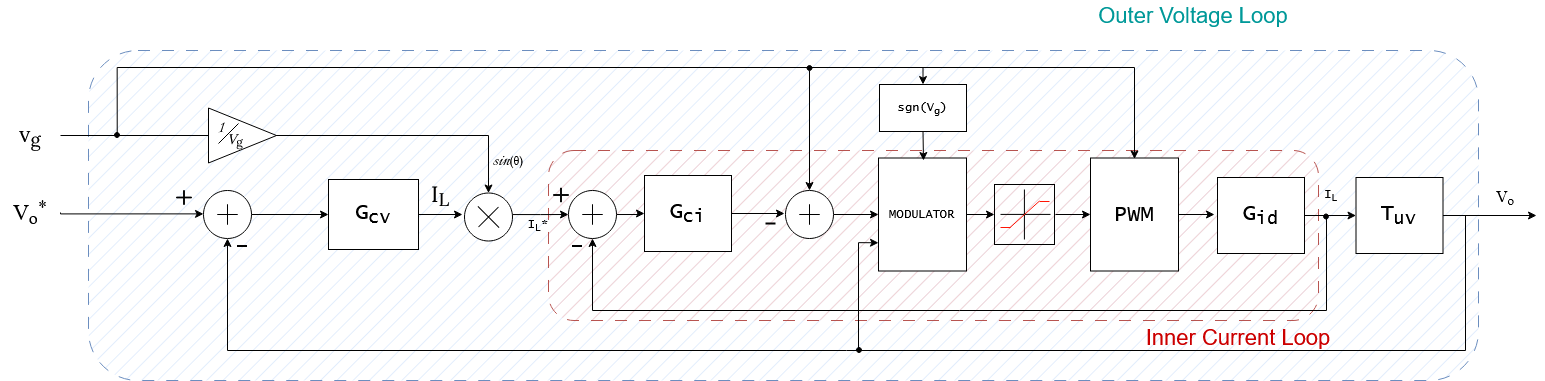
\includegraphics[width=0.8\linewidth]{figures/PI_PR_scheme(22).drawio.png}
    \caption{Cascaded PI/PR Control Scheme}
    \label{fig:PI_PR_scheme}
\end{figure*}
To find how the error evolves over time, we subtract the steady-state dynamics in (\ref{eq:steady-state}) from the averaged model system dynamics in (\ref{averaged_model}):
{\small
\begin{align*}
    L \dot{e}_1 &= -r_f e_1 + \text{sgn}(v_g) \left[ (1-u_0)V_0^* - (1-u)\bar{v}_c \right] =\\
    &= -r_f e_1 + \text{sgn}(v_g) \left[ -(1-u)e_2 + \Delta u V_0^* \right]
\end{align*}
}
\begin{align*}
    C \dot{e}_2 &= -\frac{e_2}{R_o} + \text{sgn}(v_g) \left[ (1-u)\bar{i}_L - (1-u_0)i_L^* \right]=\\
    &= -\frac{e_2}{R_o} + \text{sgn}(v_g) \left[ (1-u)e_1 - \Delta u i_L^* \right]
\end{align*}
Thus, the error dynamics of the system can be represented as:
\begin{equation}
\begin{cases} 
L\dot{e_1} = -r_f e_1 - \operatorname{sgn}(v_g)\left[-(1-u)e_2 + \Delta{u}V^*_o \right]\\
C\dot{e_2} = -\frac{e_2}{R_o} + \operatorname{sgn}(v_g)\left[(1-u)e_1 - \Delta{u}i^*_L\right]
\end{cases}
\end{equation}

Substitute the derived error dynamics back into the Lyapunov derivative $\dot{V}(e)$:
\begin{align}
    \dot{V}(e) ={}& e_1 \left( -r_f e_1 + \text{sgn}(v_g)\left[-(1-u)e_2 + \Delta u V_0^*\right] \right) \nonumber \\
    & + e_2 \left( -\frac{e_2}{R_o} + \text{sgn}(v_g)\left[(1-u)e_1 - \Delta u i_L^*\right] \right)
\end{align}
Expanding this leaves:
\begin{equation}
    \dot{V}(e) = -r_f e_1^2 - \frac{e_2^2}{R_o} + \Delta u \cdot \text{sgn}(v_g) \left[  e_1 V_0^* -e_2 i_L^* \right]
\end{equation}

For the system to be globally asymptotically stable, Lyapunov's theorem requires $\dot{V}(e) < 0$. The first two terms are strictly negative, so we must force the third term to be negative. We can guarantee this by choosing the control law for $\Delta u$ as:
\begin{equation}\label{eq:LY_control}
    \Delta u = -K_c \text{sgn}(v_g) \left[ e_1 V_0^* - e_2 i_L^* \right], \quad K_c > 0
\end{equation}
Substituting this back yields a strictly negative derivative, proving stability:
\begin{equation}\label{eq:der_LY}
    \dot{V}(e) = -r_f e_1^2 - \frac{e_2^2}{R_o} - K_c \left( \text{sgn}(v_g) \right)^2 \left[  e_1 V_0^* - e_2 i_L^* \right]^2 < 0
\end{equation}

Finally, we derived the steady-state feedforward control $u_0$ from the reference dynamics in (\ref{eq:steady_state_control}). Hence, the overall expression of the switching function
can be written as:
{\small
\begin{equation}
    u = u_o + \Delta{u} = 1 - \frac{V^*_o}{R_o \text{sgn}(v_g)i^*_L}  - K_c \text{sgn}(v_g) \left[ e_1 V_0^* - e_2 i_L^* \right]
\end{equation}
}


%------------------------------------------------
\subsection{Cascaded PI/PR Control Strategy}

The control strategy for the converter employs a cascaded architecture, heavily relying on the principle of frequency separation between two distinct control loops. To achieve proper decoupling, the inner current loop is designed to be much faster than the outer voltage loop. This ensures that the slow outer loop is perceived as an open loop from the fast inner loop standpoint, significantly simplifying the overall system synthesis. The overall control scheme is shown in Fig. \ref{fig:PI_PR_scheme}.

\subsubsection{Inner Current Loop Control}

The primary objective of the inner control loop is to regulate the duty-cycle to shape the inductor current. In a stationary reference frame, the current reference $I_L^*(s)$ is a time-varying AC sinusoidal signal. If a standard Proportional-Integral (PI) controller were used, its finite gain at the AC grid frequency would inevitably lead to a steady-state phase lag and amplitude tracking errors. 

To overcome this limitation, a Proportional-Resonant (PR) controller is utilized. The PR controller provides theoretically infinite gain exactly at the fundamental grid frequency, forcing the actual inductor current to perfectly track the AC reference with zero steady-state error and no phase shifting. The generalized $s$-domain form of the PR controller is given by:

\begin{equation}
    G_{ci}(s) = K_p + K_R \frac{s}{s^2 + \omega_R^2}
\end{equation}

where $K_p$ is the proportional gain, $K_R$ is the gain of the resonant part, and $\omega_R$ is the resonant frequency (tuned strictly to the grid frequency, e.g., $2\pi \cdot 50\text{ Hz}$). The bode plot of $G_{ci}$ is shown in Fig. \ref{fig:bode_PR}.

\begin{figure}
    \centering
    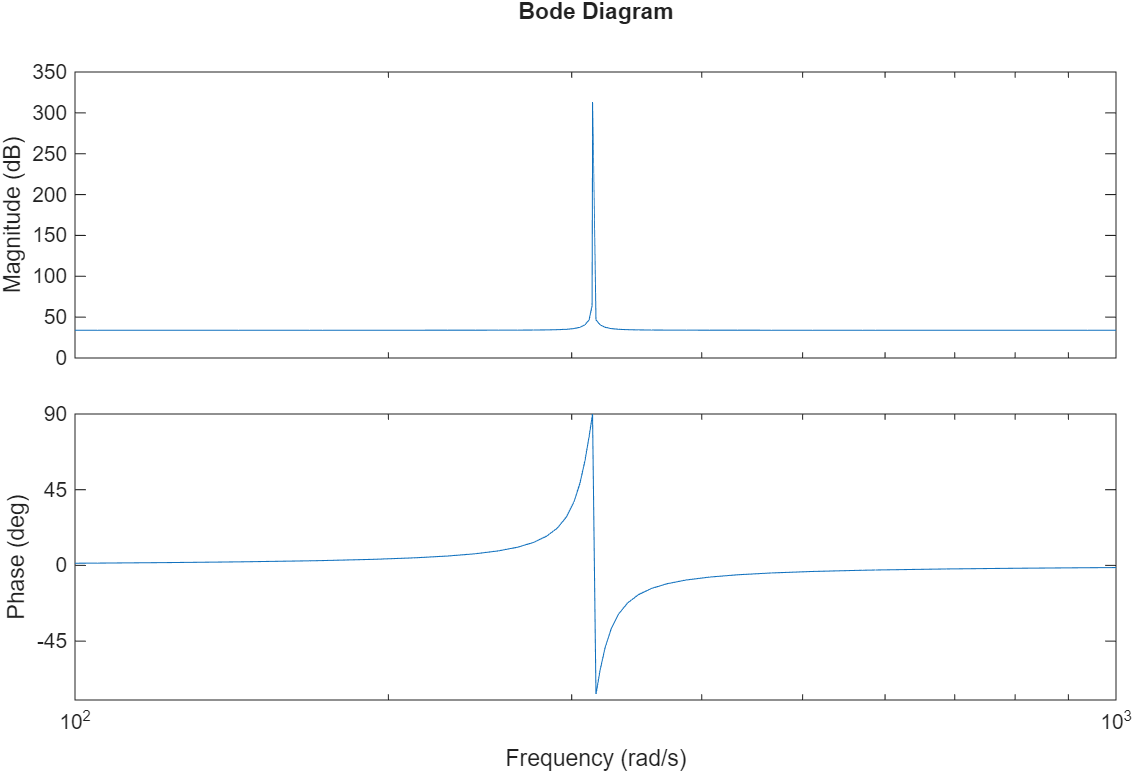
\includegraphics[width=\linewidth]{bode_PR.png}
    \caption{Bode plot of $G_{ci}$}
    \label{fig:bode_PR}
\end{figure}

The resulting transfer function of the current system in closed-loop is:

\begin{equation}
    G_{i\_CL}(s) = \frac{I_L(s)}{I_L^*(s)} = \frac{G_{ci}(s) G_{id}(s)}{1 + G_{ci}(s) G_{id}(s)}
\end{equation}

where $G_{id}(s)$ represents the plant transfer function from the duty cycle to the inductor current.

\subsubsection{Outer Voltage Loop Control}

The outer loop is responsible for regulating the DC output voltage. Because the target reference ($V_c^*$) is a flat DC value, a standard PI controller, denoted as $G_{cv}(s)$, is perfectly adequate. The integral term provides infinite gain at DC ($s = 0$), guaranteeing zero steady-state error for the output voltage. 

Furthermore, the intentionally low bandwidth of this loop ensures the complete rejection of the $100\text{ Hz}$ double-line-frequency voltage ripple inherent to single-phase PFCs, preventing it from distorting the inner loop's current reference. The voltage error signal is processed by the PI controller governed by:

\begin{equation}
    G_{cv}(s) = K_{pv} + \frac{K_{iv}}{s}
\end{equation}

where $K_{pv}$ is the proportional gain, and $K_{iv}$ is the integral gain used to set the zero frequency in combination with $K_{pv}$.


The transfer function of the complete voltage system in closed-loop is formulated as:

\begin{equation}
    G_{v\_CL}(s) = \frac{\text{V}_o(s)}{V^*_o(s)} = \frac{G_{cv}(s) G_{i\_Cl}(s) T_{uv}(s)}{1 + G_{cv}(s) G_{i\_CL}(s) T_{uv}(s)}
\end{equation}

where $T_{uv}(s)$ represents the plant transfer function for the voltage loop.



\subsection{Phasors Domain Approach}
\begin{figure*}[htp]
    \centering
    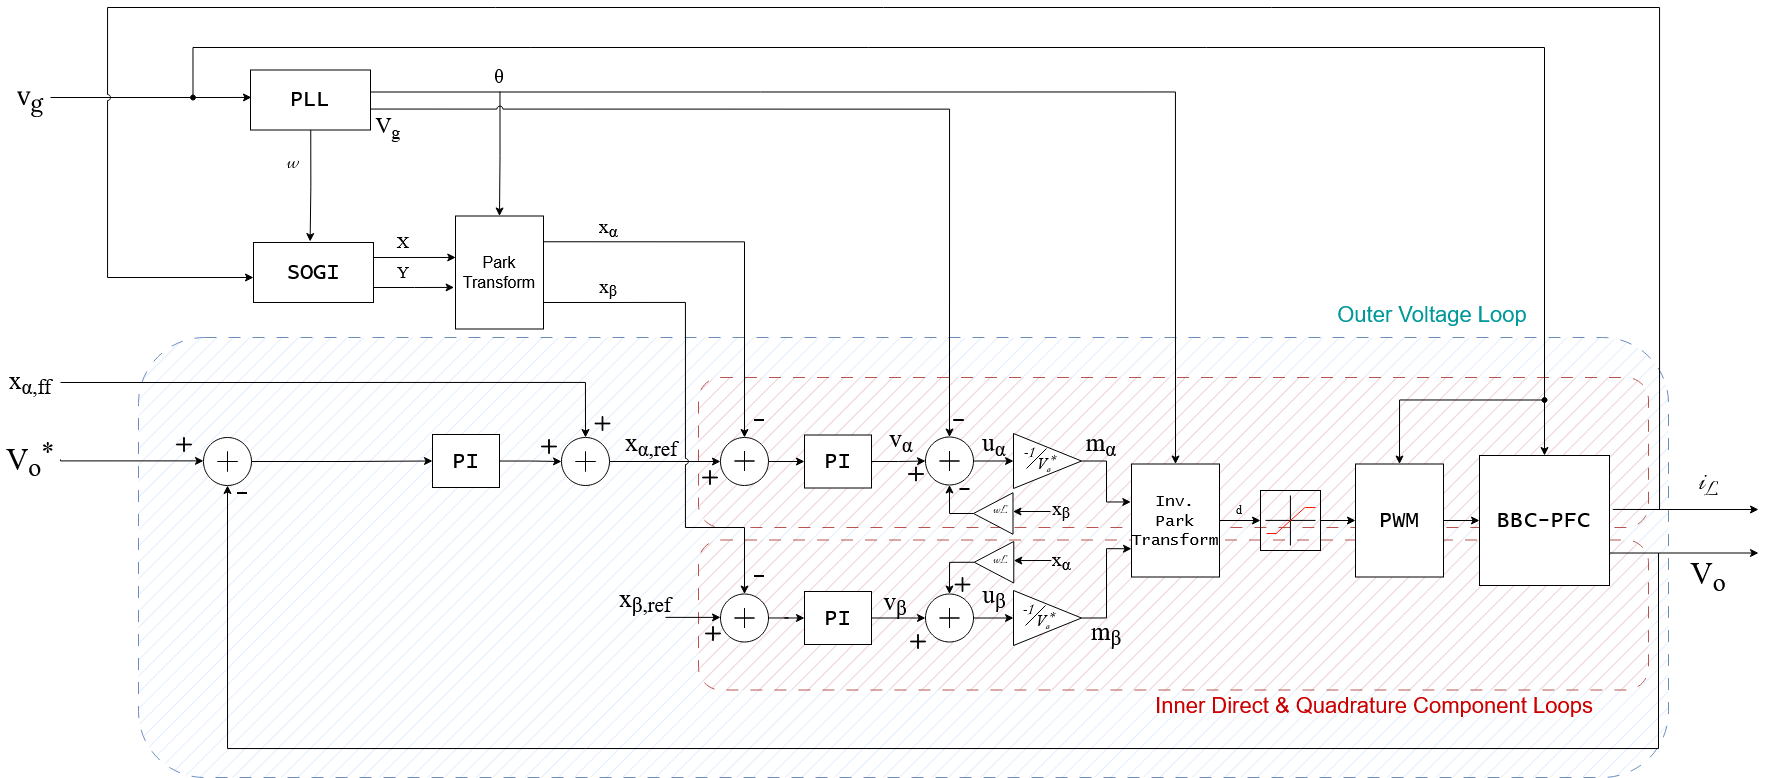
\includegraphics[width=0.8\linewidth]{figures/phasor_control_scheme(3).drawio.png}
    \caption{Phasors Domain Control Scheme}
    \label{fig:phasors_domain_control_scheme}
\end{figure*}
\subsubsection{Modeling Active and Reactive Components}
Starting with the averaged model:
\begin{equation}
    \begin{cases} 
        \frac{d\bar{x}_1}{dt} = \frac{-r_f \bar{x}_1 - \text{sgn}(v_g(t))(1-d(t))\bar{x}_2 + v_g(t)}{L} \\[8pt]
        \frac{d\bar{x}_2}{dt} = \frac{\text{sgn}(v_g(t))(1-d(t))\bar{x}_1 - \frac{\bar{x}_2}{R_o}}{C}
    \end{cases}
\end{equation}

We can define the modulating signal as:
{\small 
\begin{equation}
m(t) = \text{sgn}(v_g(t)) (1 - d(t))
\end{equation}
}
Thus, the system can be written as:
% \begin{equation}
%     \begin{cases} 
%         L \dot{\bar{x}}_1 = -r_f \bar{x}_1 - \text{sgn}(v_g)(1-d(t))\bar{x}_2 + v_g \\[8pt]
%         C \dot{\bar{x}}_2 = \text{sgn}(v_g)(1-d(t))\bar{x}_1 - \frac{\bar{x}_2}{R_o}
%     \end{cases}
% \end{equation}

% \begin{equation}
%     \text{sgn}(v_g)(1 - d(t)) = 
%     \begin{cases} 
%         0, & m(t) < 0 \\ 
%         1, & m(t) > V_p \\ 
%         \frac{m(t)}{V_p}, & 0 \le m(t) \le V_p 
%     \end{cases}
% \end{equation}

% where $V_p = 1$. Substituting this into our state equations:
\begin{equation}
    \begin{cases} 
        L \dot{\bar{x}}_1 = -r_f \bar{x}_1 + v_g(t) - m\bar{x}_2 \\[8pt]
        C \dot{\bar{x}}_2 = m\bar{x}_1 - \frac{\bar{x}_2}{R_o}
    \end{cases}
\end{equation}
We define the grid voltage and state variables in the phasors domain as:
{\small
\begin{align}\label{direct_quad}
    v_g(t) &= V_{g} \sin(\omega t) \\
    \bar{x}_1(t) &= X_1(t) \sin(\omega t + \varphi(t)) \\ \bar{x}_1(t) &= \bar{x}_\alpha(t) \sin(\omega t) + \bar{x}_\beta(t) \cos(\omega t) \\
    \bar{x}_\alpha(t) &= X_1(t) \cos(\varphi(t)), \quad \bar{x}_\beta(t) = X_1(t) \sin(\varphi(t))
\end{align}
}

We define the control variable in the phasor domain as follows:
{\small
\begin{align}
    m(t) &= M(t) \sin(\omega t + \gamma(t)) \\ m(t)&= m_\alpha \sin(\omega t) + m_\beta \cos(\omega t) \\
    m_\alpha(t) &= M(t) \cos(\gamma(t)), \quad m_\beta(t) = M(t) \sin(\gamma(t))\label{quad_ph}
\end{align}
}

Substituting the expressions from (\ref{direct_quad}) through (\ref{quad_ph}) in the first state equation, and separating the terms multiplying $\cos(\omega t)$ and $\sin(\omega t)$, respectively, we obtain two state equations:
\begin{equation}
    \begin{cases} 
        L \dot{\bar{x}}_\alpha = -r_f \bar{x}_\alpha + \omega L \bar{x}_\beta + V_g - m_\alpha \bar{x}_2 \\[8pt]
        L \dot{\bar{x}}_\beta = -r_f \bar{x}_\beta - \omega L \bar{x}_\alpha - m_\beta \bar{x}_2
    \end{cases}
\end{equation}

In the third equation, we can write the term $m(t)\bar{x}_1(t)$ as follows:

{\small
\begin{equation}
\begin{split}
&m(t)\bar{x}_1(t) = m_\alpha \bar{x}_\alpha \sin^2(\omega t) + m_\alpha \bar{x}_\beta \sin(\omega t)\cos(\omega t) +\\
&+ m_\beta \bar{x}_\alpha \sin(\omega t) \cos(\omega t) + m_\beta \bar{x}_\beta \cos^2(\omega t) \\
&= m_\alpha \bar{x}_\alpha \left(\frac{1 - \cos(2\omega t)}{2}\right) + \frac{m_\alpha \bar{x}_\beta \sin(2\omega t)}{2} + \\
&+\frac{m_\beta \bar{x}_\alpha \sin(2\omega t)}{2}+
 m_\beta \bar{x}_\beta \left(\frac{1 + \cos(2\omega t)}{2}\right)
\end{split}
\end{equation}
}
Neglecting the terms at twice the grid voltage frequency, we have only the scalar product left:
\begin{equation}
    m(t)\bar{x}_1(t) \cong \frac{1}{2} \langle [m_\alpha, m_\beta], [\bar{x}_\alpha, \bar{x}_\beta] \rangle
\end{equation}

Yielding the full dynamic phasor model:
\begin{equation}
    \begin{cases} 
        L \dot{\bar{x}}_\alpha = -r_f \bar{x}_\alpha + \omega L \bar{x}_\beta + V_g - m_\alpha \bar{x}_2 \\[8pt]
        L \dot{\bar{x}}_\beta = -r_f \bar{x}_\beta - \omega L \bar{x}_\alpha - m_\beta \bar{x}_2 \\[8pt]
        C \dot{\bar{x}}_2 = \frac{1}{2}(m_\alpha \bar{x}_\alpha + m_\beta \bar{x}_\beta) - \frac{\bar{x}_2}{R_o}
    \end{cases}
\end{equation}
\subsubsection{Control Scheme}

% The system employs a cascaded control architecture consisting of a slow outer voltage loop and two fast inner current loops. 

The overall control scheme is shown in Fig. \ref{fig:phasors_domain_control_scheme}. The outer loop consists of a PI controller that generates an inductor current peak value to compensate for the voltage error. This value is summed with a feedforward inductor current reference value.

Because at steady-state the inductor current is in-phase with the grid voltage ($\bar{x}_{\beta_{,ref}} = 0$), we can write the state equations at steady-state as:
\begin{equation} \label{ph-steady-state}
    \begin{cases} 
        r_f \bar{x}_\alpha = V_g - m_\alpha V_o^* \\[8pt]
        \omega L \bar{x}_\alpha = -m_\beta V_o^* \\[8pt]
        \frac{m_\alpha \bar{x}_\alpha}{2} = \frac{V_o^*}{R_o}
    \end{cases}
\end{equation}

Substituting the third equation into the first equation, we get the following:
\begin{equation}
\frac{r_f \bar{x}_\alpha^2}{2} = \frac{V_g \bar{x}_\alpha}{2} - \frac{(V_o^*)^2}{R_o}
\end{equation}

Thus, we get a solution for $\bar{x}_\alpha$ which is the equivalent in the phasors domain of (\ref{eq:peak_current}).
This value becomes the feedforward reference value for the active component of the inductor current, denoted as $x_{\alpha_{,ff}}$:
\begin{equation}\label{eq:x_alpha_fwd}
    \bar{x}_{\alpha_{,ff}} = \frac{1}{2} \frac{V_g}{r_f} \left[ 1 - \sqrt{1 - 8 \frac{(V_o^*)^2 r_f}{V_g^2 R_o}} \right]
\end{equation}
The sum of the output of the PI controller with the feedforward inductor current active component is the reference value of the active component of the inductor current, denoted with $x_{\alpha_,{ref}}$.
\begin{figure}[htp]
    \centering
    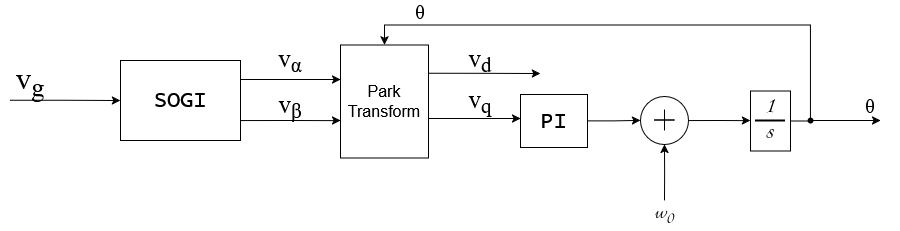
\includegraphics[width=1\linewidth]{figures/PLL.drawio.png}
    \caption{PLL Block}
    \label{fig:PLL}
\end{figure}

The inner current control loops are used to regulate the active and reactive components of the inductor current, respectively. 

First, a Phase-Locked Loop (PLL) extracts the instantaneous grid angle, $\theta$, the angular frequency, $\omega$, and the peak grid voltage amplitude, $V_g$. To construct a two-dimensional stationary vector from a scalar single-phase measurement, a Second-Order Generalized Integrator (SOGI) is employed. The SOGI processes the measured inductor current, $i_L(s)$, yielding two orthogonal signals in the stationary frame, defined in the control scheme as $x(t)$ and $y(t)$. The transfer functions for the direct and quadrature signals are given by:
\begin{align}
    H_x(s) &= \frac{X(s)}{I_L(s)} = \frac{k\omega s}{s^2 + k\omega s + \omega^2} \\
    H_y(s) &= \frac{Y(s)}{I_L(s)} = \frac{k\omega^2}{s^2 + k\omega s + \omega^2}
\end{align}
where $k$ is the SOGI damping factor (gain), usually set to $k = \sqrt{2}$, and $\omega$ is the grid angular frequency given by the PLL.
\begin{figure}[htp]
    \centering
    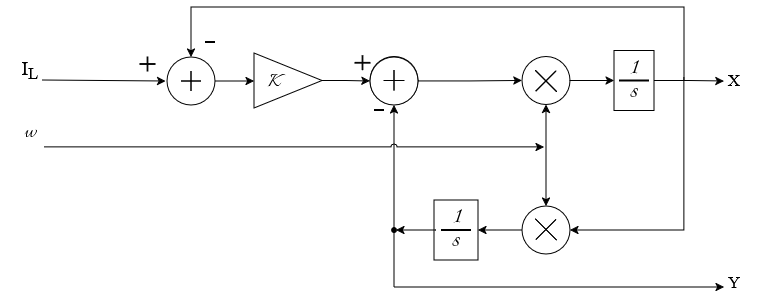
\includegraphics[width=1\linewidth]{figures/SOGI.png}
    \caption{SOGI-QSG block}
    \label{fig:SOGI}
\end{figure}

Thus, we may write:
 \begin{align}
    x(t) &= i_L(t) \\
    y(t) &= i_L(t) \cdot e^{-j\pi/2}
\end{align} 


The PLL and SOGI block are represented in Fig. \ref{fig:PLL} and \ref{fig:SOGI}, respectively.
To align the active current component perfectly with the grid voltage sine wave, a Park transformation is applied to the stationary components $x$ and $y$. This maps the AC signals to the rotating reference frame, denoted in the system as $\bar{x}_\alpha$ (active/direct current) and $\bar{x}_\beta$ (reactive/quadrature current):
\begin{subequations}\begin{align}
    \bar{x}_\alpha &=  x \sin(\theta) - y \cos(\theta)\label{eq:x_alpha} \\
    \bar{x}_\beta &= x \cos(\theta) + y \sin(\theta)\label{eq:x_beta}
\end{align}\end{subequations}
In steady-state operation at unity power factor, $\bar{x}_\alpha$ becomes a flat DC value representing the peak fundamental current, and $\bar{x}_\beta$ regulates to exactly zero.

At steady-state we will have:
\begin{subequations}\begin{align}
    L \frac{d\bar{x}_\alpha}{dt} &= -r_f \bar{x}_\alpha + \omega L \bar{x}_\beta + V_g - m_\alpha V_o^* \label{eq:plant_alpha} \\
    L \frac{d\bar{x}_\beta}{dt} &= -r_f \bar{x}_\beta - \omega L \bar{x}_\alpha - m_\beta V_o^* \label{eq:plant_beta}
\end{align}\end{subequations}

% We can now substitute this expression in (\ref{ph-steady-state}) and solve for $m_\alpha$ and $m_\beta$. Finally, we have:
% \begin{equation}
%     M = \sqrt{m_\alpha^2 + m_\beta^2} \quad ; \quad \gamma = \tan^{-1}\left(\frac{m_\beta}{m_\alpha}\right)
% \end{equation}


Equations \eqref{eq:plant_alpha} and \eqref{eq:plant_beta} reveal cross-coupling between the axes due to the $\omega L$ terms, as well as a disturbance from the grid voltage $V_g$. To allow independent tuning of the $\bar{x}_\alpha$ and $\bar{x}_\beta$ current loops, an algebraic feedforward decoupling network is implemented. 

Let $v_\alpha$ and $v_\beta$ be the outputs of the PI current compensators. To linearize the plant for the PI controllers, we define the control effort variables $u_\alpha$ and $u_\beta$ as:
\begin{subequations}\begin{align}
    u_\alpha &\triangleq V_g - m_\alpha V_o^* \\  u_\beta &\triangleq -m_\beta V_o^*
\end{align}\end{subequations}

The final decoupled duty-cycle control laws are:

\begin{subequations}\begin{align}
    m_\alpha &= \frac{V_g - v_\alpha + \omega L \bar{x}_\beta}{V_o^*}  \label{eq:decouple_alpha} \\
    m_\beta &= \frac{- v_\beta - \omega L \bar{x}_\alpha}{V_o^*} \label{eq:decouple_beta}
\end{align}\end{subequations}
where $V_o^*$ is the output voltage reference. Applying these control laws mathematically cancels the cross-coupling, reducing the plant seen by the PI controllers to a simple, independent first-order system: $G(s) = \frac{1}{sL + r_f}$. The mathematical steps used to derive these results are presented in Appendix B.
The final stage translates the DC control commands back into a physical AC duty cycle. An inverse Park transformation recombines the decoupled $m_\alpha$ and $m_\beta$ signals using the instantaneous grid angle $\theta$:
\begin{equation}\label{eq:inv_park}
    m(t) = m_\alpha \sin(\theta) + m_\beta \cos(\theta)
\end{equation}
The physical duty cycle $d(t)$ is taken equal to:
\begin{equation}\label{eq:duty}
    d(t) = 1 - \frac{m(t)}{\text{sgn}(v_g)}
\end{equation}
This duty cycle is passed through a saturation block, which outputs a bounded duty cycle ($0 \le d \le d_{max}$), and then to the Pulse Width Modulation (PWM) generator to drive the converter's active switches.


\section{Experimental Setup: PLECS Models}

\begin{figure}[htp]
    \centering
    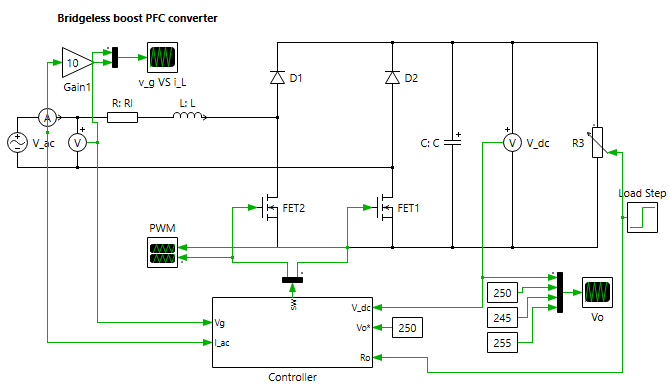
\includegraphics[width=1\linewidth]{figures/Bridgeless_boost_PFC_converter_1.png}
    \caption{Bridgeless boost PFC converter}
    \label{fig:bbc_pfc}
\end{figure}
In this section, we present the details related to the \textit{Controller} subsystems, which were implemented in PLECS to test the control strategies previously analysed.
First, the Bridgeless Boost PFC Converter, subject of this study, was modelled. These models can be downloaded from \cite{GitHub}. The same circuit, then, is used to run the simulations. This circuit is represented in \ref{fig:bbc_pfc}. Then, three separate controller subsystems were developed to simulate the performance of the three different control strategies under test. Each of these controllers operates in the continuous time domain. Thus, continuous-time transfer functions are used in the implementations.
The same system parameters were used across the simulations, with differences only in the parameters used for specific tasks related to the given control strategy implemented. These parameters are reported in Table \ref{tab:tab_1}.
\begin{table}[htp]
        \centering
        \caption{Circuit Parameters}
        \label{tab:tab_1}
        \pgfplotstabletypeset[normal,
            columns/Parameter/.style={column name={\textbf{Parameter}}},
            columns/Value/.style={column name={\textbf{Value}}}
        ]{ %
        Parameter    & Value \\
        {$v_{g}(t)$} & {$V_{g} \sin(\omega t)$ V} \\ 
        {$V_g$}      & {$110\sqrt{2}$ V} \\ 
        {$\omega$}   & {$2\pi f$ rad/s} \\
        {$f$}        & {$50.0$Hz} \\
        {$R_l$}      & {$0.02$$\Omega$} \\
        {$R_o$}      & {$125$$\Omega$} \\
        {$C$}        & {$500\mu$F} \\
        {$L$}        & {$1$mH} \\
        {$V^*_o$}    & {$250$V}\\
        }
    \end{table}
To test the responsiveness of the system to changes in the load, a load step is used, which doubles the nominal output resistance $R_o$ at time $t=400$ms, similarly to what was proposed in \cite{TU}.

\subsection{Lyapunov Based Controller}
\begin{figure}[htp]
    \centering
    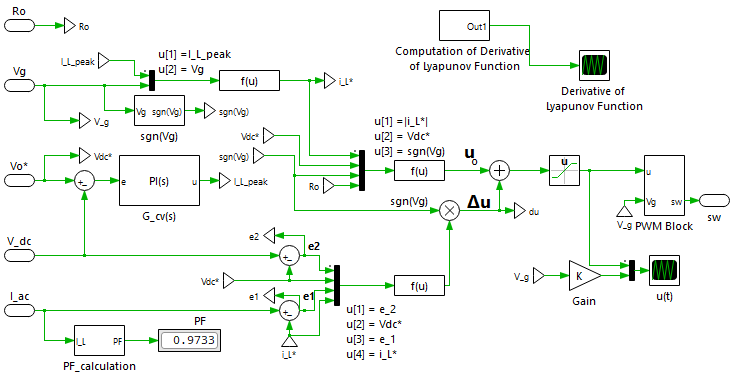
\includegraphics[width=1\linewidth]{figures/controlly_1.png}
    \caption{Lyapunov Based Controller}
    \label{fig:LY}
\end{figure}
The Lyapunov-based controller is represented in Fig. \ref{fig:LY}. 

The controller takes four inputs, namely the inductor current $i_L$, the output voltage $V_o$, the reference DC voltage $V^*_o$, and the input voltage $v_g$. A custom \textit{sgn(Vg)} block is used to compute the sign of the input voltage, which is used both in the PWM block and for the control variable $\Delta u$. 

The PI controller is used in the outer voltage loop to compensate for the voltage error, based on (\ref{eq:G_cv}). The output of this PI controller is the peak inductor current. 
The reference inductor current is generated by implementing (\ref{eq:reference_ind_curr}) with a function block.

Below the outer voltage loop, the inductor current and the output voltage are used to generate the error states $e_1$ and $e_2$ used in the inner Lyapunov-based control loop, as defined in (\ref{eq:error_state}). Therefore, yet another function block, together with $\text{sgn}(v_g)$, generates the control action $\Delta u$ according to (\ref{eq:LY_control}). At the same time, the feedforward action $u_o$ is computed by implementing (\ref{eq:steady_state_control}), and is summed to $\Delta u$, yielding the total control action $u$.

\begin{table}[htp]
        \centering
        \caption{Lyapunov-based Controller Parameters}
        \label{tab:LY}
        \pgfplotstabletypeset[normal,
            columns/Parameter/.style={column name={\textbf{Parameter}}},
            columns/Value/.style={column name={\textbf{Value}}}
        ]{ %
        Parameter        & Value \\
        \topmidheader{2}{Outer PI Controller $G_{cv}(s)$}
        % {$G_{mcv}$}      & {$0.026\Omega^{-1}$} \\ 
        {$K_p$}          & {$0.1$} \\
        {$K_i$}          & {$10$} \\ 
        % {$\omega_{zcv}$} & {$2 \pi f_{zcv}$ rad/s} \\
        % {$f_{zcv}$}      & {$66.78$Hz} \\
        \midheader{2}{Inner Lyapunov Control Loop}
        {$K_c$}          & {$0.002$} \\
        }
    \end{table}
Thus, the two control actions are summed to give the resulting control $u$. This control action passes through the saturation block, whose upper limit and lower limit are set to 0.95 and 0.1, respectively.
The saturated control is used in the PWM block to generate the actual switching signal that commands the MOSFETs, $Q_1$ and $Q_2$, of the converter.
Finally, a custom block, named \textit{Computation of Derivative of Lyapunov Function}, is used to compute the derivative of the Lyapunov function, as represented by (\ref{eq:der_LY}).

The values used to set the parameters $K_p$ and $K_i$ of the PI controller and the gain $K_c$ for the Lyapunov-based stability method are reported in Table \ref{tab:LY}.


\subsection{Cascaded PI/PR Controller}
\begin{figure}[htp]
    \centering
    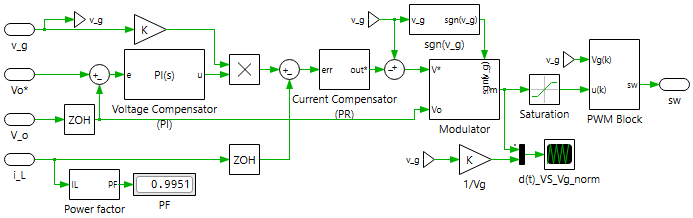
\includegraphics[width=1\linewidth]{figures/PI_PR_Controller.png}
    \caption{Cascaded PI/PR Controller}
    \label{fig:PLECS_PI_PR_controller}
\end{figure}

The cascaded PI/PR controller is represented in Fig. \ref{fig:PLECS_PI_PR_controller}. The inputs of this controller are the same as those of the Lyapunov-based controller.

This controller is based on an example that is available among the \textit{Demo Models} in PLECS, named "\textit{Bridgeless boost PFC Converter}" \cite{PLECS}. The controller used in this example was designed to work with a different converter topology, including two inductors and, more importantly, two clamping diodes. Thus, the way the switches $Q_1$ and $Q_2$ are controlled cannot be applied straightforwardly to our converter. To allow the control scheme to work with the topology chosen for this study, which lacks the clamping diodes, the custom block \textit{sgn(Vg)} was used to fine-tune the control action depending on the polarity of the input voltage. This is achieved in the \textit{Modulator} custom block.

The parameters used to set the proportional and integral gains of the PI and the PR are reported in Table \ref{tab:PI_PR}.
\begin{table}[htp]
    \centering
    \caption{PI and PR Compensator Parameters}
    \label{tab:PI_PR}
    \pgfplotstabletypeset[normal,
        columns/Parameter/.style={column name={\textbf{Parameter}}},
        columns/Value/.style={column name={\textbf{Value}}}
    ]{ %
    Parameter    & Value \\
    \topmidheader{2}{PI Voltage Compensator}
    {$K_p$}      & {$0.1$} \\ 
    {$K_i$}      & {$10$} \\ 
    \midheader{2}{PR Current Compensator}
    {$K_p$}      & {$50$} \\
    {$K_r$}      & {$1000$} \\
    }
\end{table}

\subsection{Phasors Domain Controller}

\begin{figure}[htp]
    \centering
    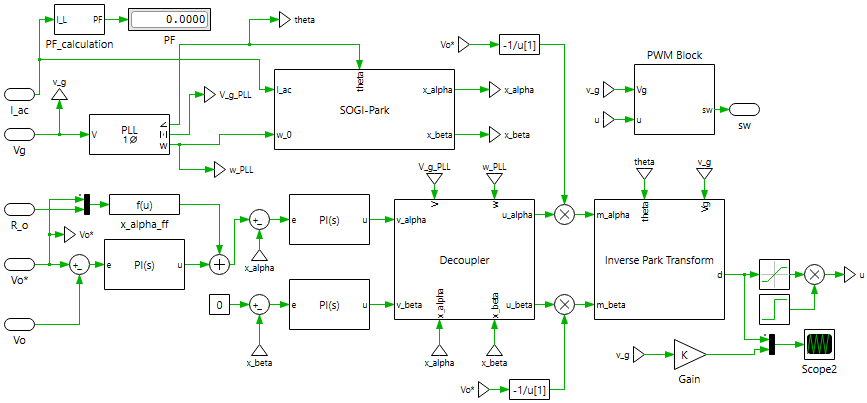
\includegraphics[width=1\linewidth]{figures/control_phasors1_6_3.png}
    \caption{Control scheme Phasors Domain Approach}
    \label{fig:control_6_3}
\end{figure}

The Phasors Domain Controller is shown in Fig. \ref{fig:control_6_3}. 
The input voltage is passed to a library block \textit{Single-Phase PLL}. This block implements an SOGI-based single-phase Phase Locked Loop (PLL). The single-phase PLL block, thus, provides at its output terminals an estimation of the input signal frequency $w_{PLL}$, signal amplitude $V_{g_{PLL}}$ and the phase-angle $\theta$. These outputs are used by the custom block \textit{SOGI-Park}, which takes the inductor current and outputs the direct and quadrature components, $x_\alpha$ and $x_\beta$, as defined in (\ref{eq:x_alpha}) and (\ref{eq:x_beta}).

The outer voltage loop uses a PI controller to compensate for the voltage error. The output of this controller is summed to the feedforward reference inductor current, generated according to (\ref{eq:x_alpha_fwd}). Then, the inner control loop uses two other PI controllers to compensate for the errors with respect to the direct and quadrature components, respectively. The output of these controllers, $v_\alpha$ and $v_\beta$, are passed to a custom block \textit{Decoupler}, which implements (\ref{eq:decouple_alpha}) and (\ref{eq:decouple_beta}). The output of this block produces $m_\alpha$ and $m_\beta$, which are fed to a custom block \textit{Inverse Park Transform}. This block uses the estimated phase-angle to generate the duty cycle according to (\ref{eq:inv_park}) and (\ref{eq:duty}).
The duty cycle, after being passed through a saturation block, is multiplied by the output of a \textit{Step} block. Indeed, it was necessary to allow the PLL to reach a stable value for the estimated phase angle before the control action generated by the PIs could be used; otherwise, the controllers would have generated aggressive control actions that would have stopped the simulation. This step block was set to generate a unit step at time $t=60$ms, which is equal to the settling time reported in the \textit{Help} for the single-phase PLL library block \cite{PLL}. 

The parameters of the PI controllers used in the controller are reported in Table \ref{tab:SRF_Parameters}.
\begin{table}[htp]
    \centering
    \caption{Phasors Controller PI Parameters}
    \label{tab:SRF_Parameters}
    \pgfplotstabletypeset[normal,
        columns/Parameter/.style={column name={\textbf{Parameter}}},
        columns/Value/.style={column name={\textbf{Value}}}
    ]{ %
    Parameter    & Value \\
    \topmidheader{2}{Outer Voltage Loop ($V_{o}$)}
    {$K_{p,v}$}  & {0.1} \\ 
    {$K_{i,v}$}  & {10} \\ 
    \midheader{2}{Inner Current Loop ($x_\alpha$ - Direct)}
    {$K_{p,\alpha}$} & {0.0001} \\
    {$K_{i,\alpha}$} & {0.002} \\
    \midheader{2}{Inner Current Loop ($x_\beta$ - Quadrature)}
    {$K_{p,\beta}$}  & {62.8} \\
    {$K_{i,\beta}$}  & {1256} \\
    }
\end{table}

\section{Experimental Results}
\begin{table}[htp]
    \centering
    \caption{PLECS Simulation Parameters}
    \label{tab:simulation_parameters}
    \pgfplotstabletypeset[normal,
        columns/Parameter/.style={column name={\textbf{Parameter}}},
        columns/Value/.style={column name={\textbf{Value}}}
    ]{ %
    Parameter              & Value \\
    \topmidheader{2}{Simulation Time}
    {Start Time}           & {$0.0$ s} \\ 
    {Stop Time}            & {$1$ s} \\
    {Load Step}            & {$400$ ms} \\
    \midheader{2}{Solver Settings}
    {Solver Type}          & {Variable-step} \\
    {Solver Algorithm}     & {auto} \\
    {Max Step Size}        & {$1$ ms}\\
    }
\end{table}

% \begin{figure*}[htbp]
%     \centering
%     % --- FIRST ROW: Subfigures 1 & 2 ---
%     % Subfigure 1: Top-left
%     \begin{subfigure}[b]{0.4\textwidth}
%         \centering
%         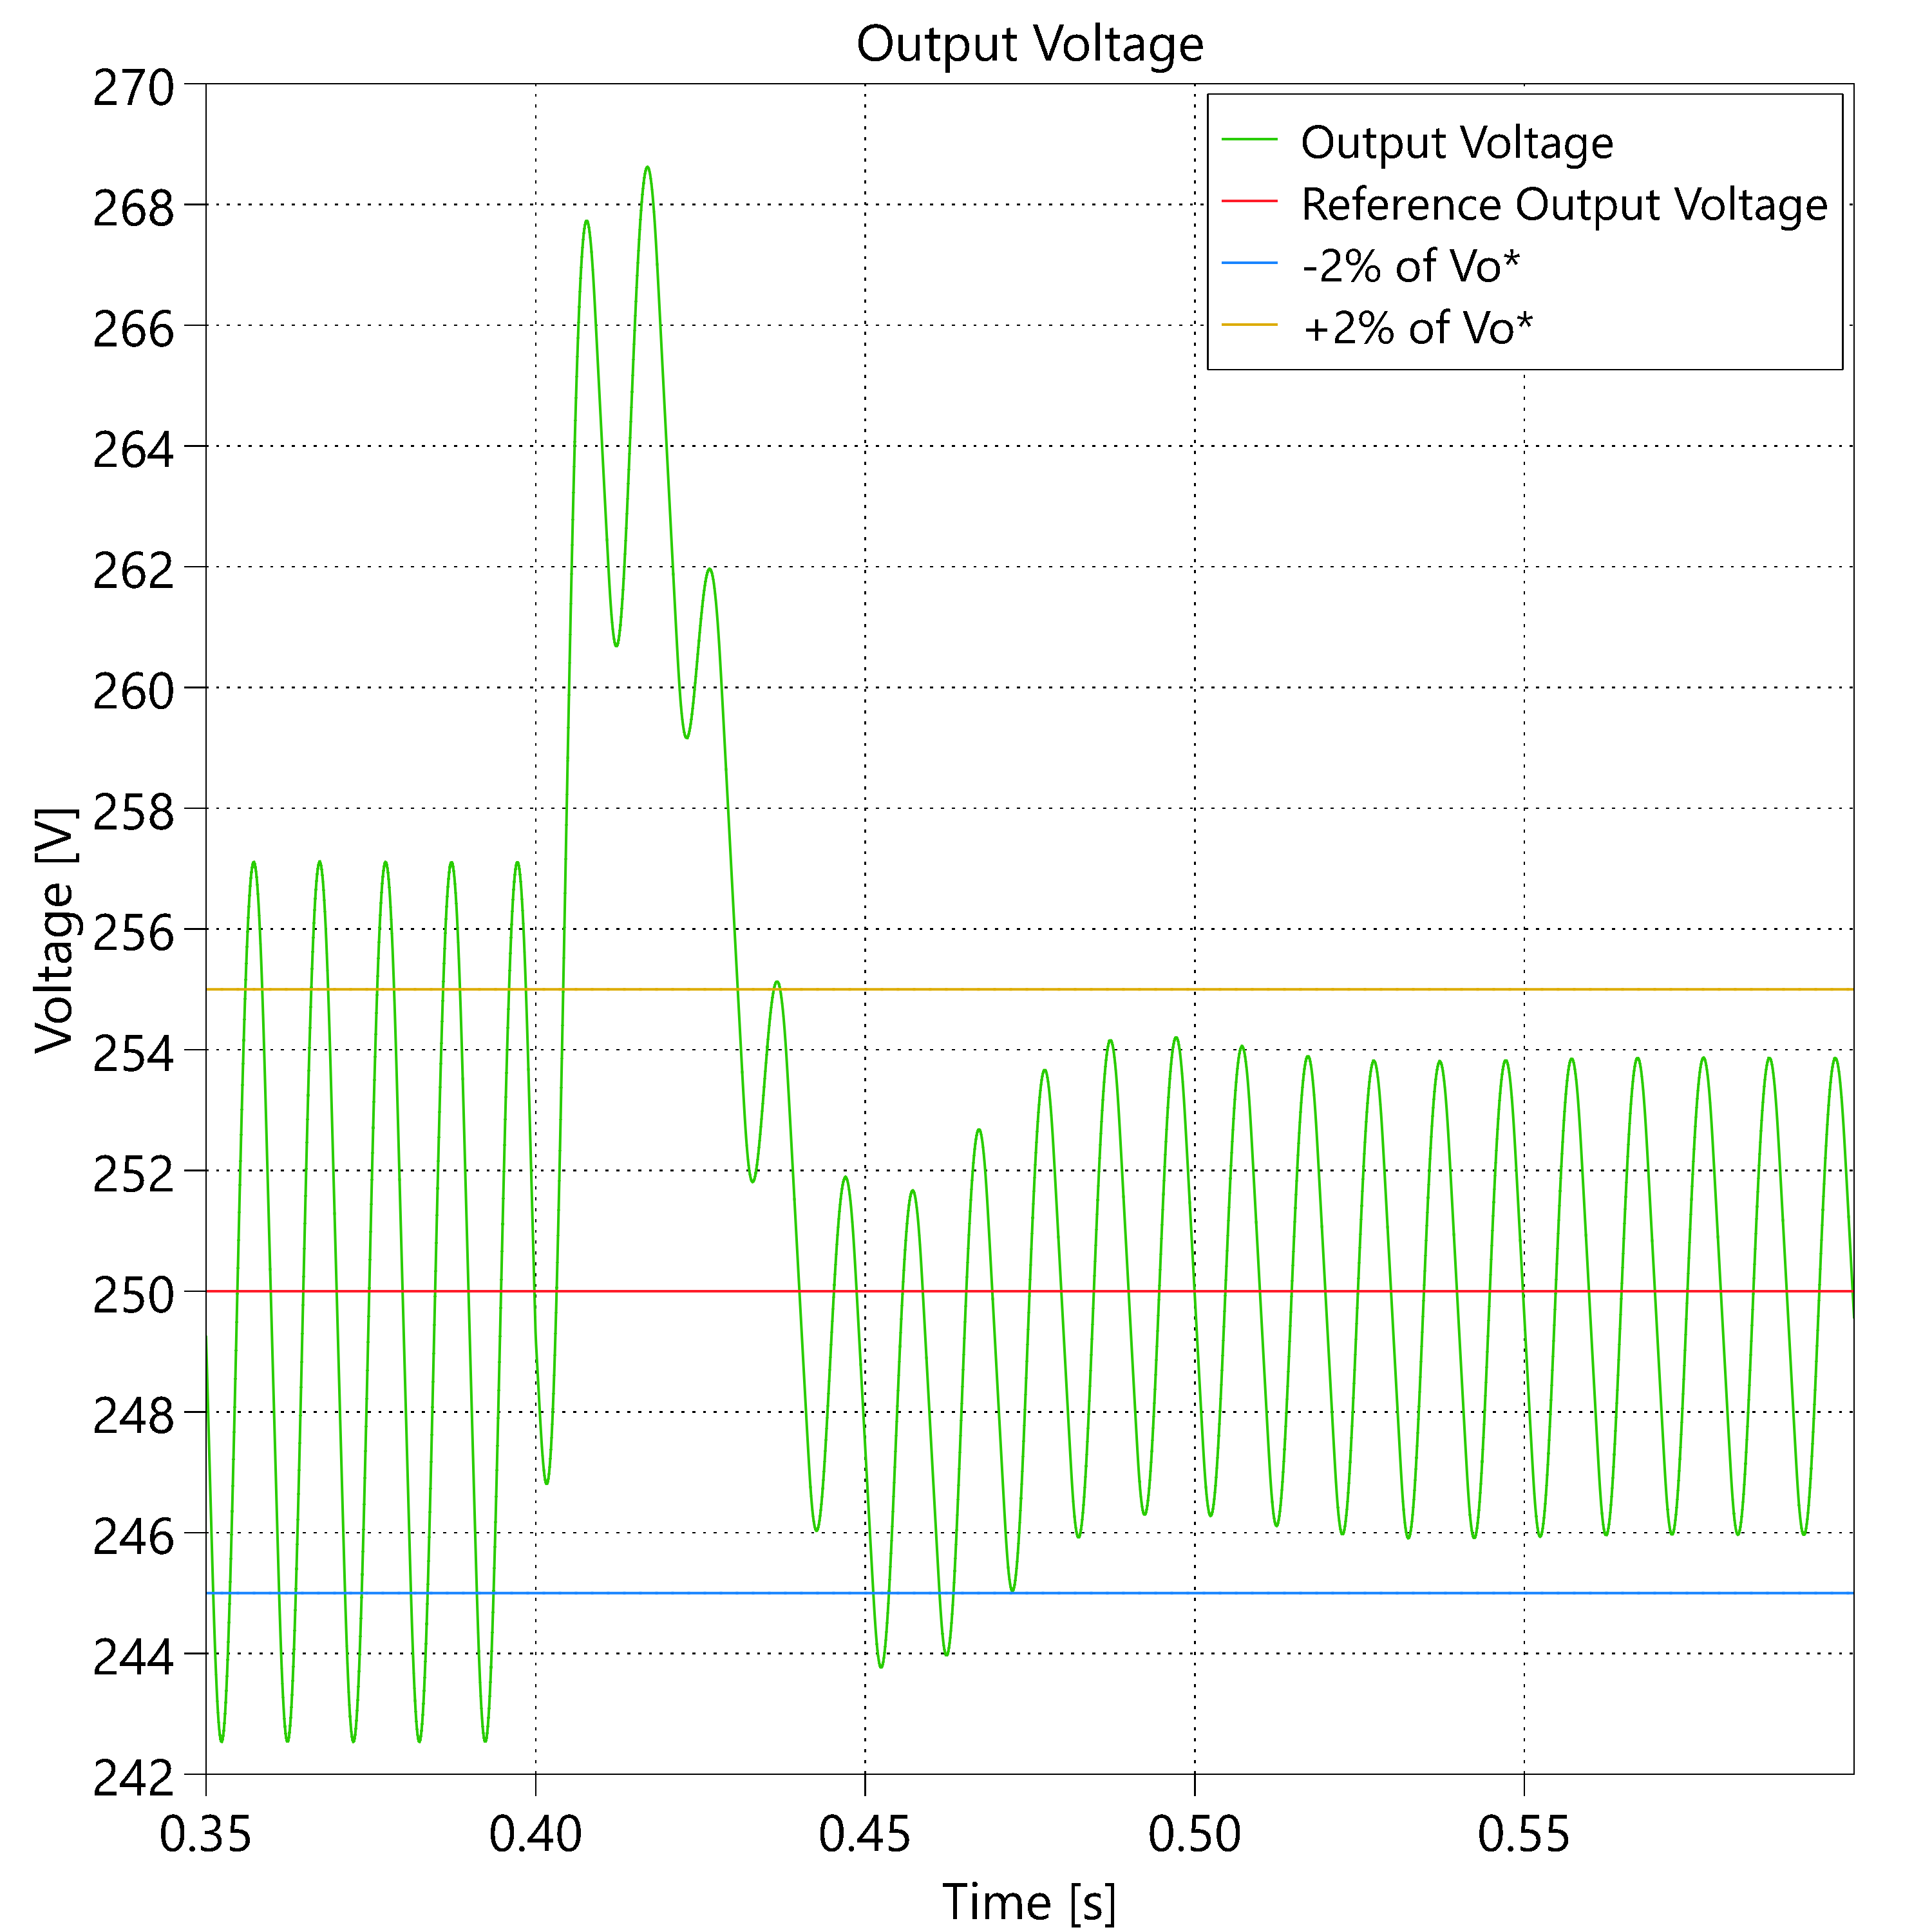
\includegraphics[width=\textwidth]{figures/LYVo1.png} % Replace with your first image filename
%         \caption{Lyapunov-based control, Voltage Regulation}
%         \label{fig:output_voltage_LY}
%     \end{subfigure}
%     \hfill % Pushes the first and second images to the page margins
%     % Subfigure 2: Top-right
%     \begin{subfigure}[b]{0.4\textwidth}
%         \centering
%         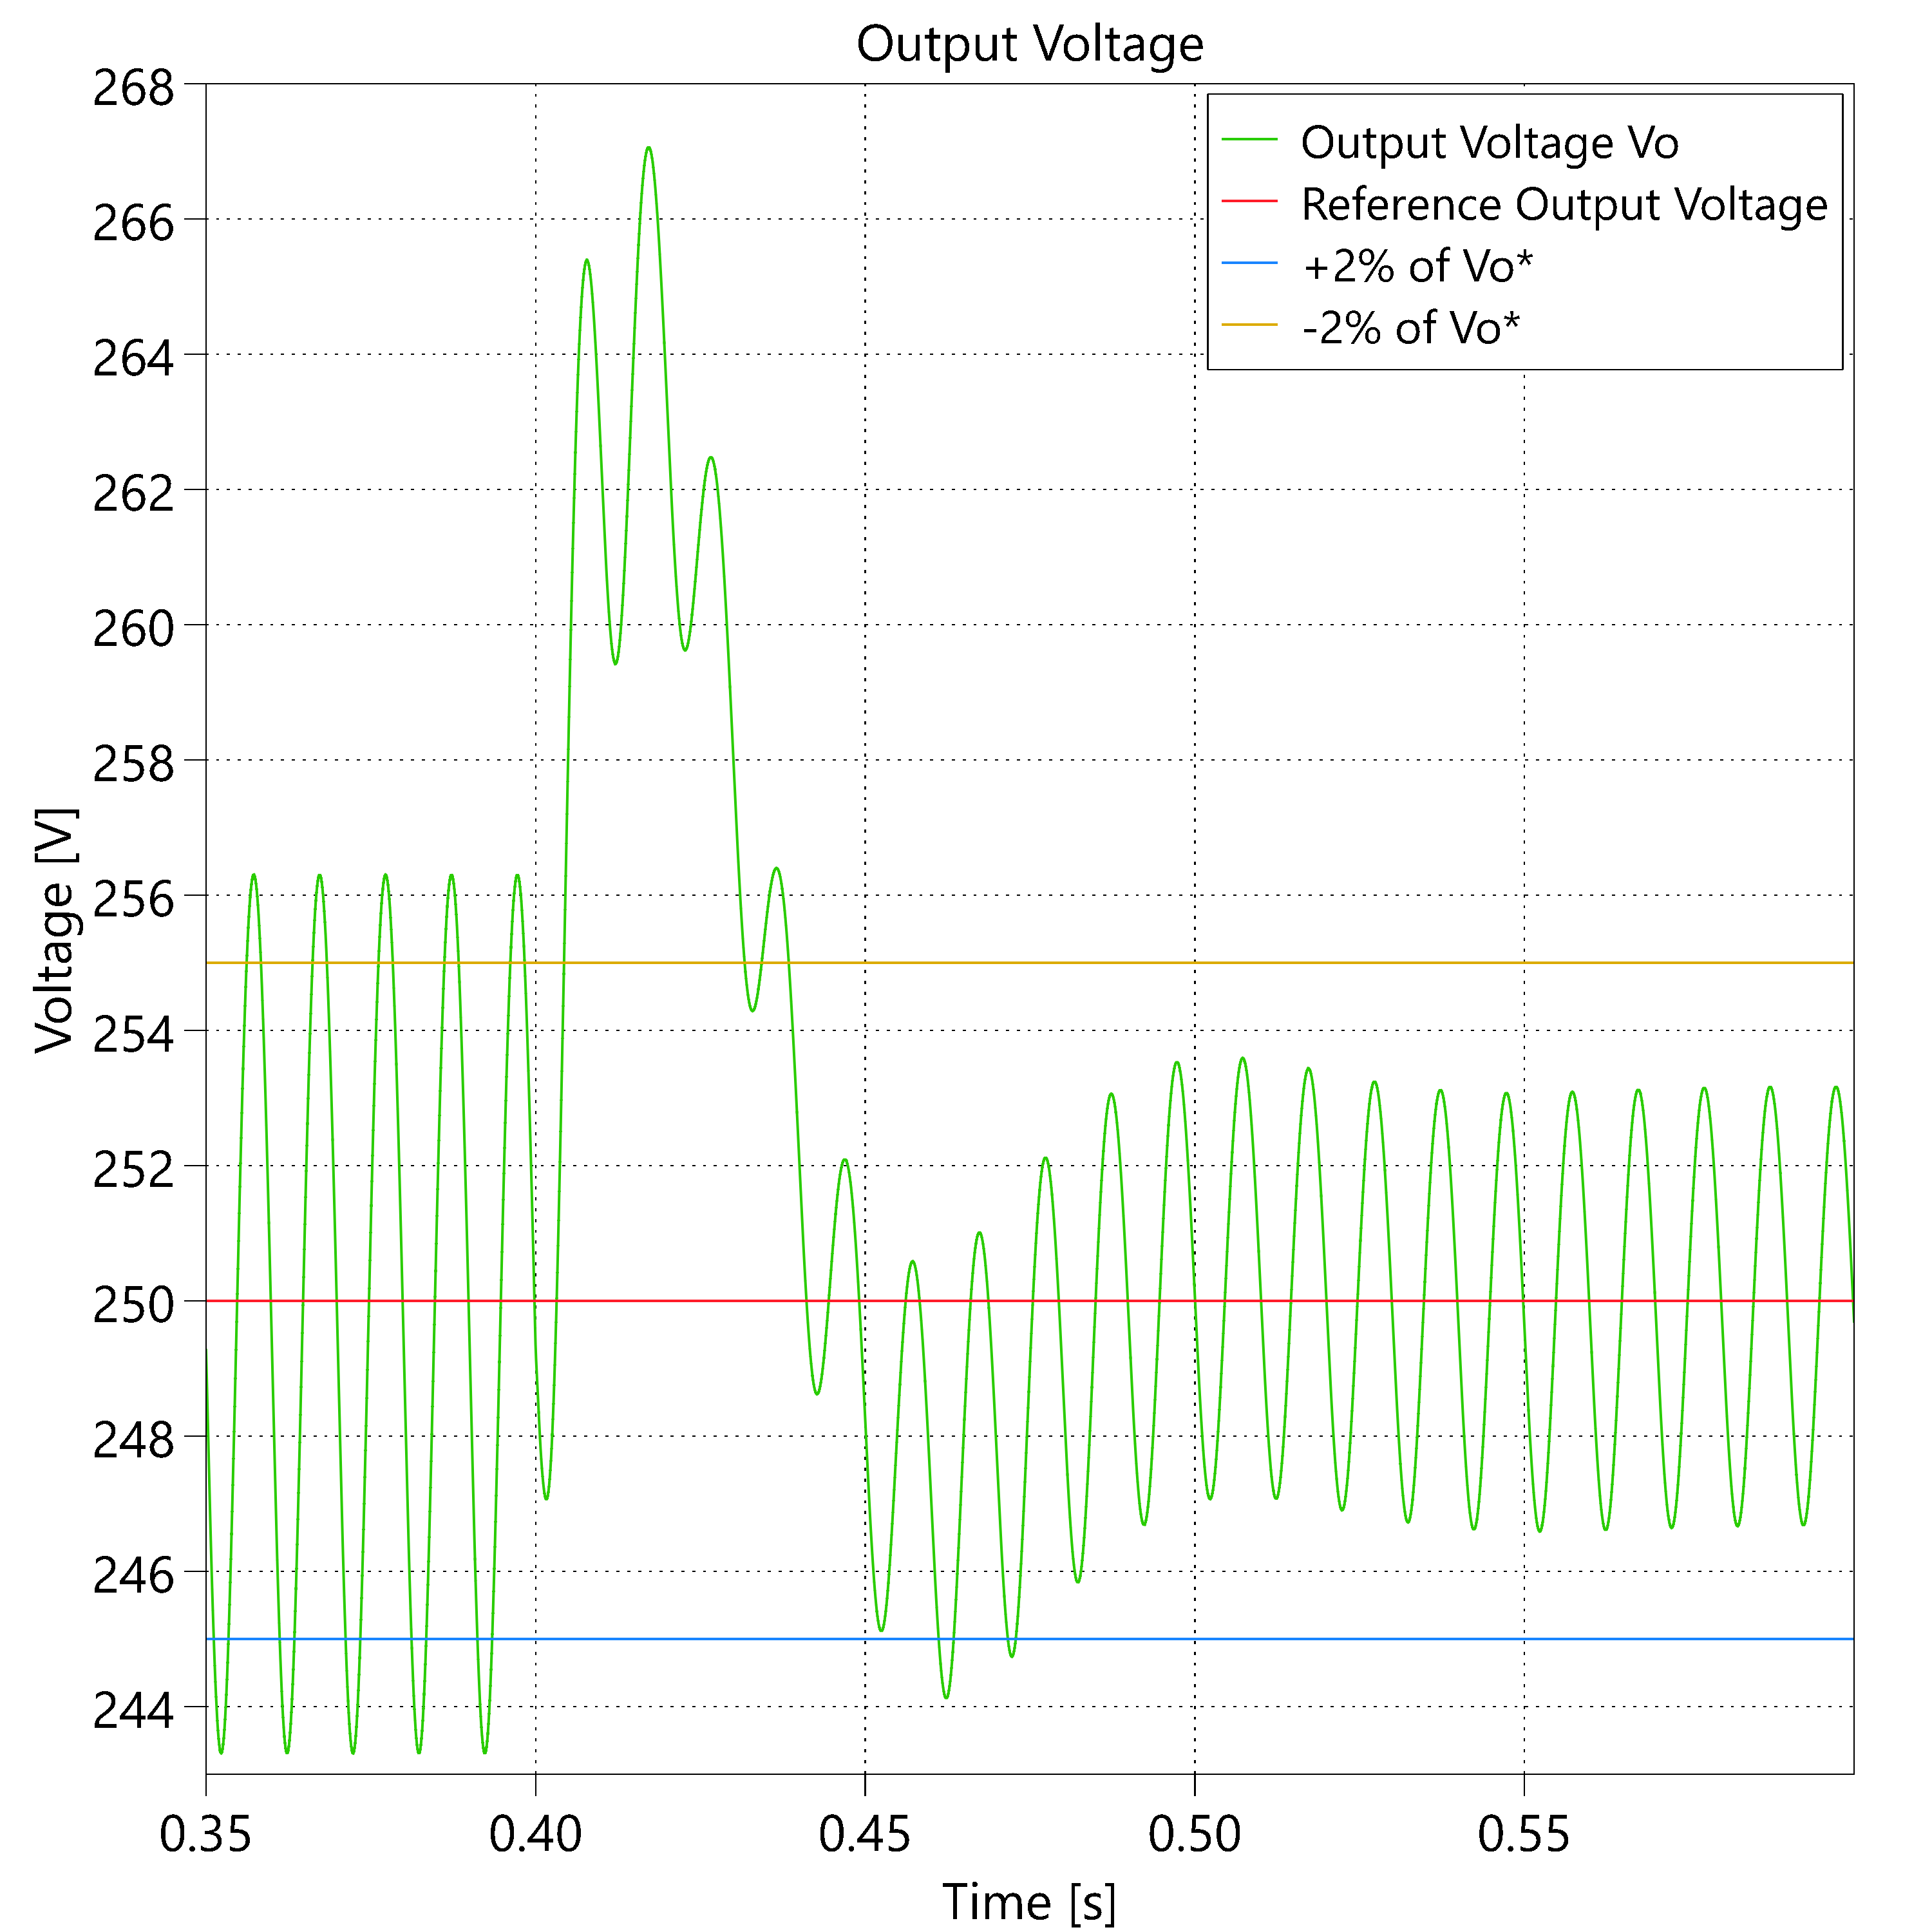
\includegraphics[width=\textwidth]{figures/piprVO.png} % Replace with your second image filename
%         \caption{PI/PR control, Voltage Regulation}
%         \label{fig:output_voltage_pipr}
%     \end{subfigure}
    
%     \vspace{2ex} % Optional: Adds a small vertical space between rows for better visuals
    
%     % --- SECOND ROW: Subfigures 3 & 4 ---
%     % Subfigure 3: Bottom-left
%     \begin{subfigure}[b]{0.4\textwidth}
%         \centering
%         
\includegraphics[width=\textwidth]{figures/Inductor_Current_VS_Input_Voltage_Lyapunov_controller.png} % Replace with your third image filename
%         \caption{Lyapunov-based control, Input Voltage vs. Inductor Current}
%         \label{fig:current_LY}
%     \end{subfigure}
%     \hfill % Pushes the third and fourth images to the page margins
%     % Subfigure 4: Bottom-right
%     \begin{subfigure}[b]{0.4\textwidth}
%         \centering
%         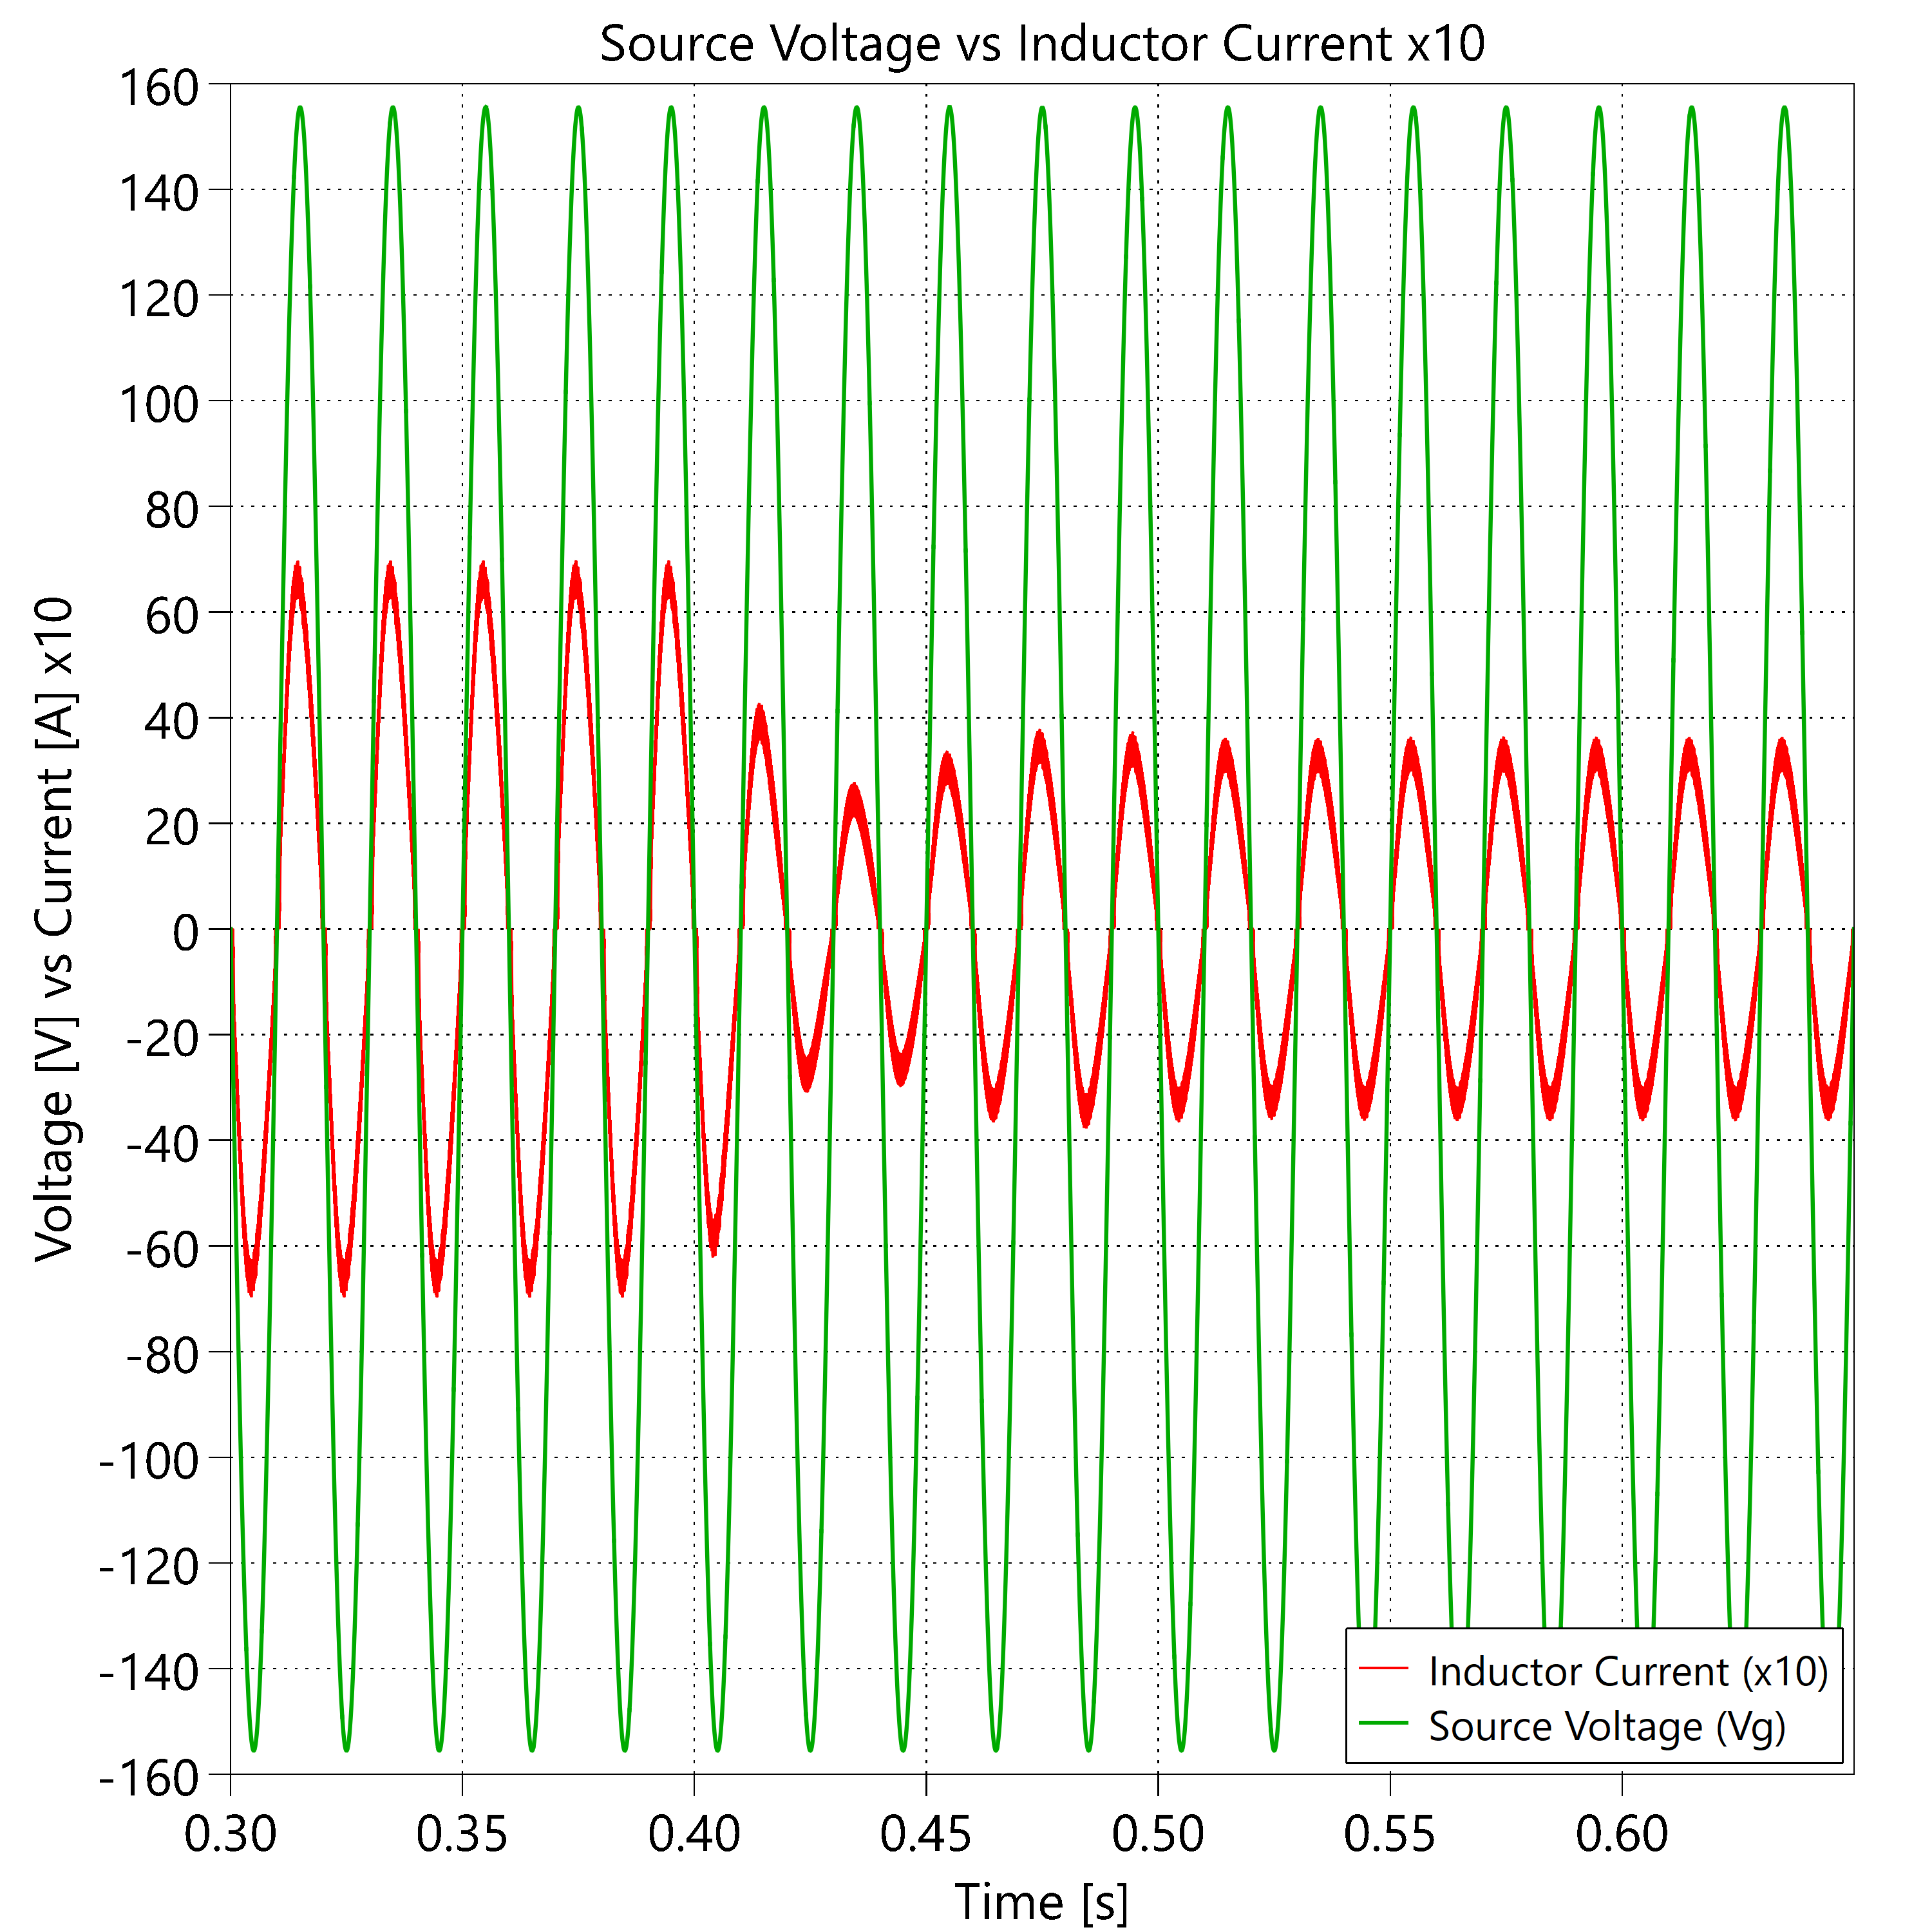
\includegraphics[width=\textwidth]{figures/pipriAC.png} % Replace with your fourth image filename
%         \caption{PI/PR control, Input Voltage vs. Inductor Current}
%         \label{fig:current_pipr}
%     \end{subfigure}

%     \vspace{2ex} % Optional: Adds a small vertical space between rows for better visuals
    
%     % --- SECOND ROW: Subfigures 3 & 4 ---
%     % Subfigure 3: Bottom-left
%     \begin{subfigure}[b]{0.4\textwidth}
%         \centering
%         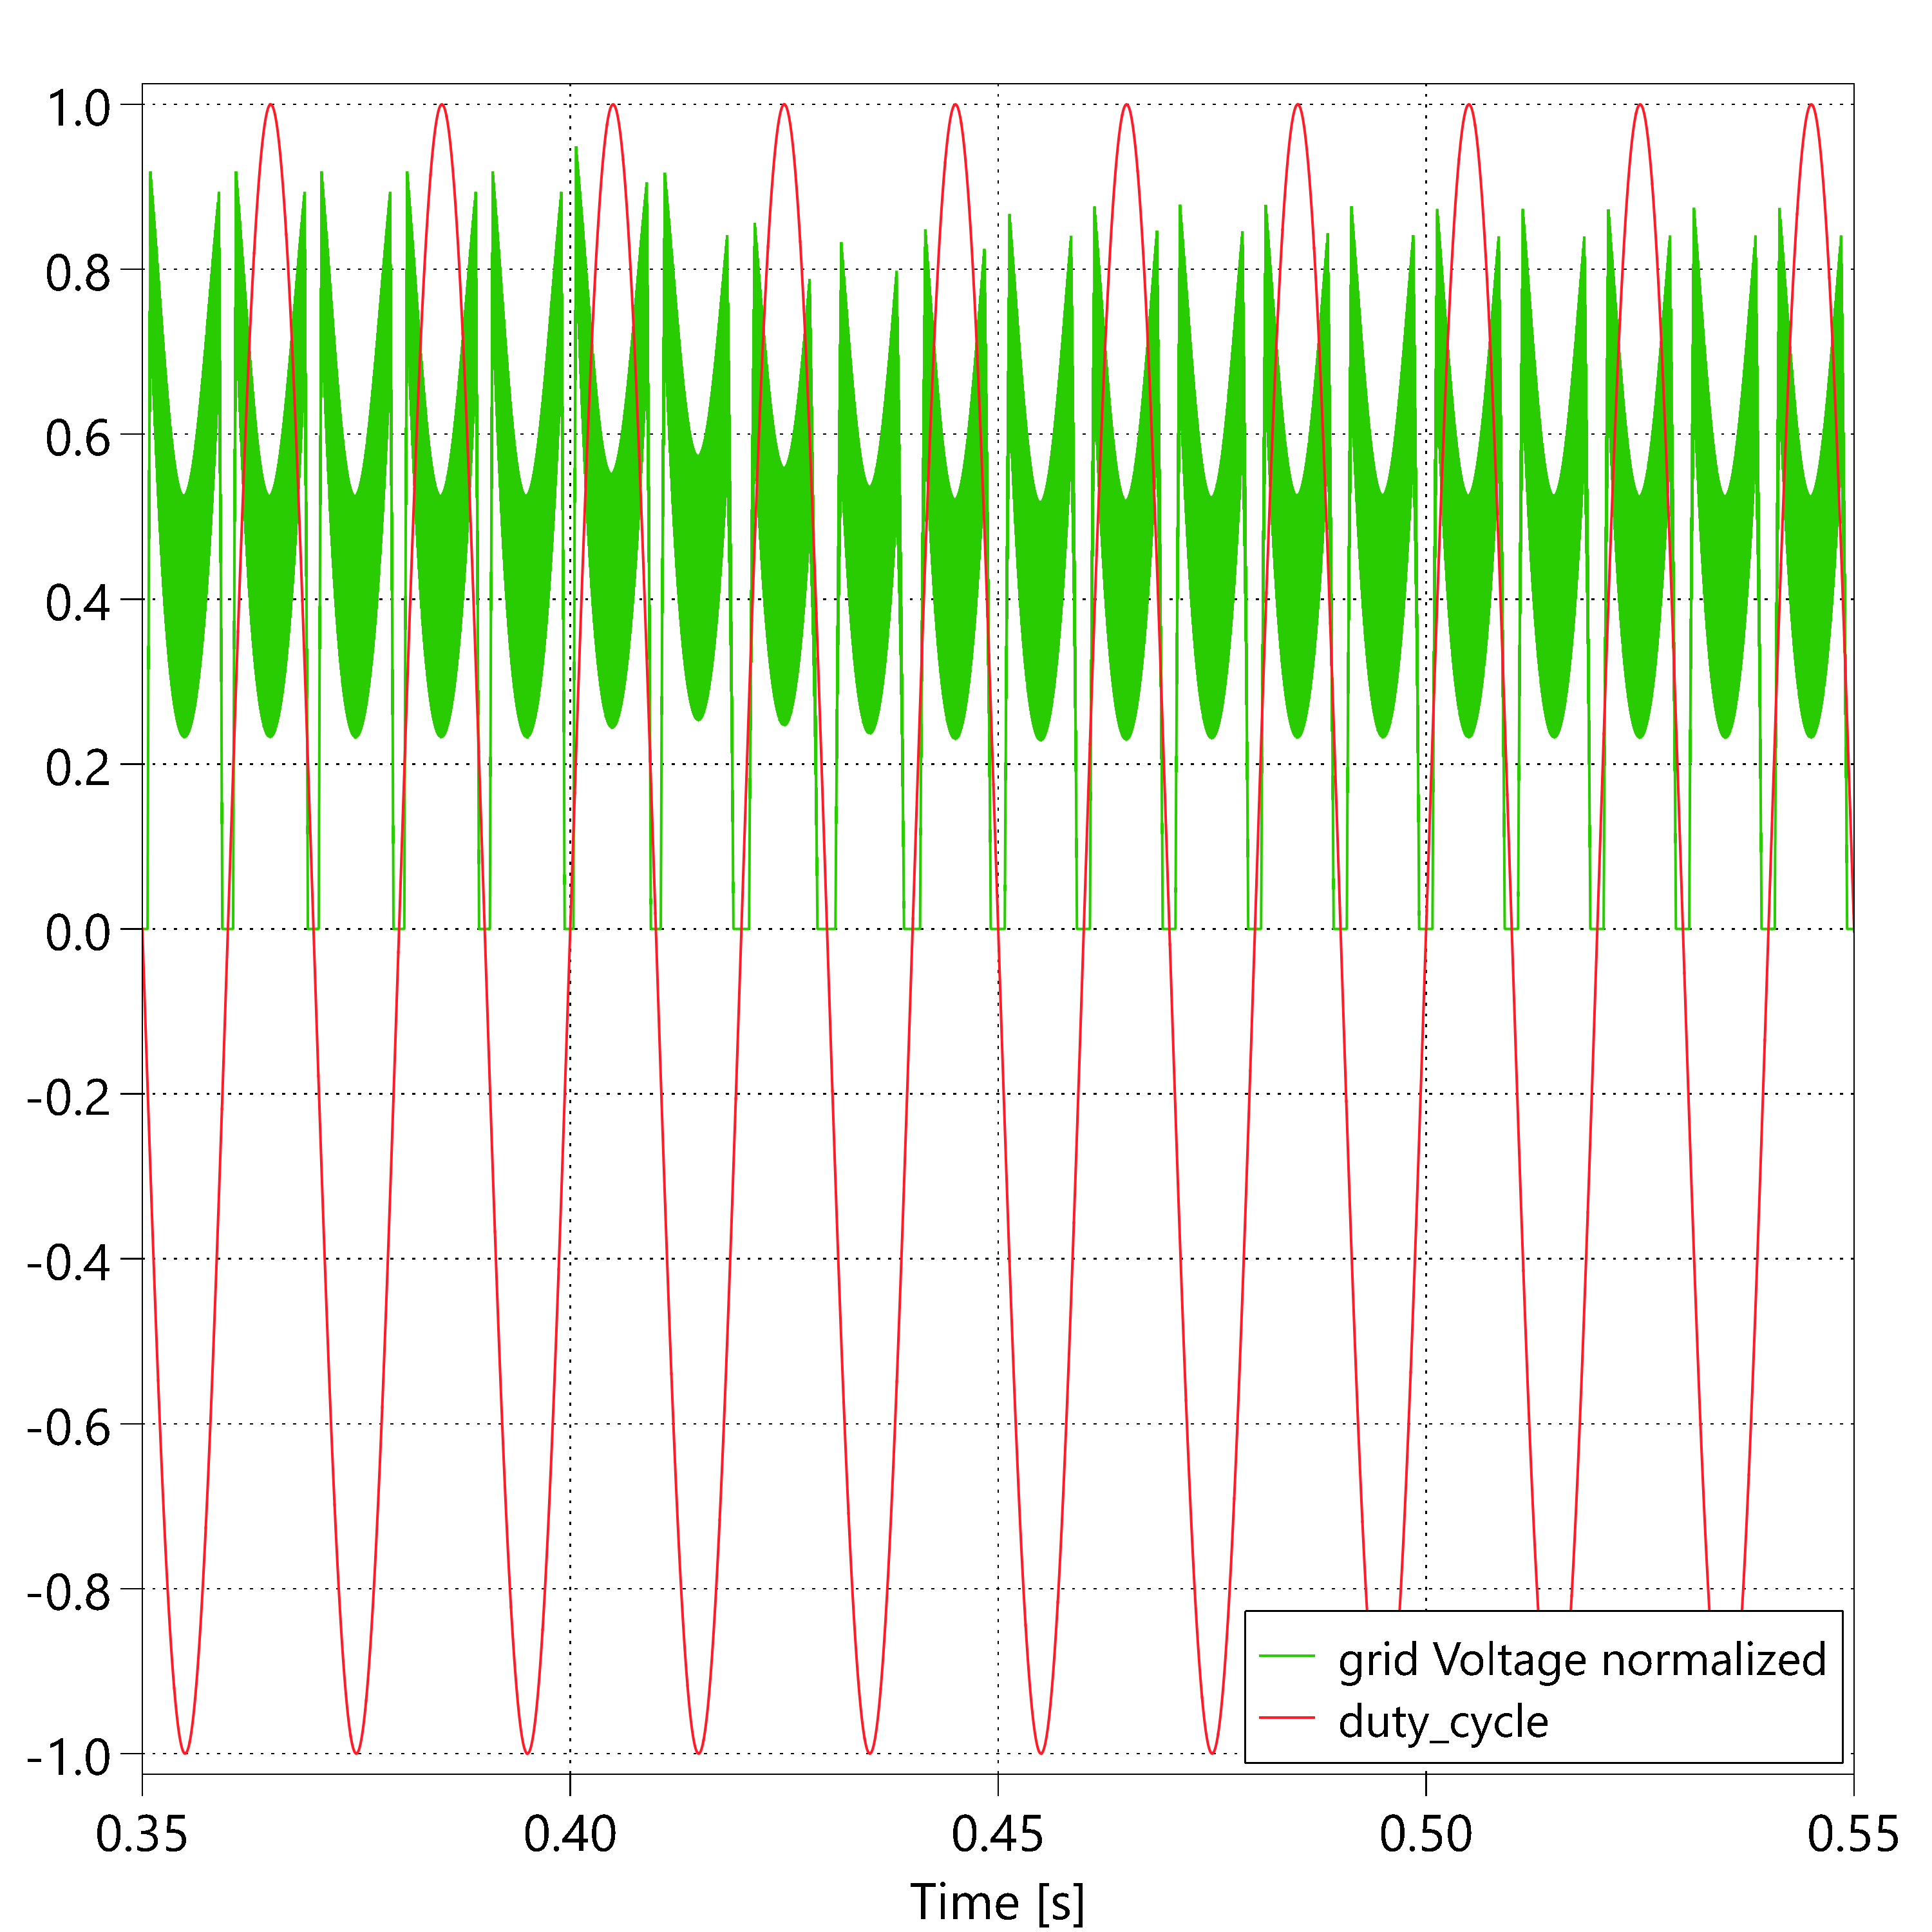
\includegraphics[width=\textwidth]{figures/DUTY_ly_1.png} % Replace with your third image filename
%         \caption{Lyapunov-based control, Comparison of Duty Cycle vs Normalized Grid Voltage}
%         \label{fig:LY_duty_cycle_LY}
%     \end{subfigure}
%     \hfill % Pushes the third and fourth images to the page margins
%     % Subfigure 4: Bottom-right
%     \begin{subfigure}[b]{0.4\textwidth}
%         \centering
%         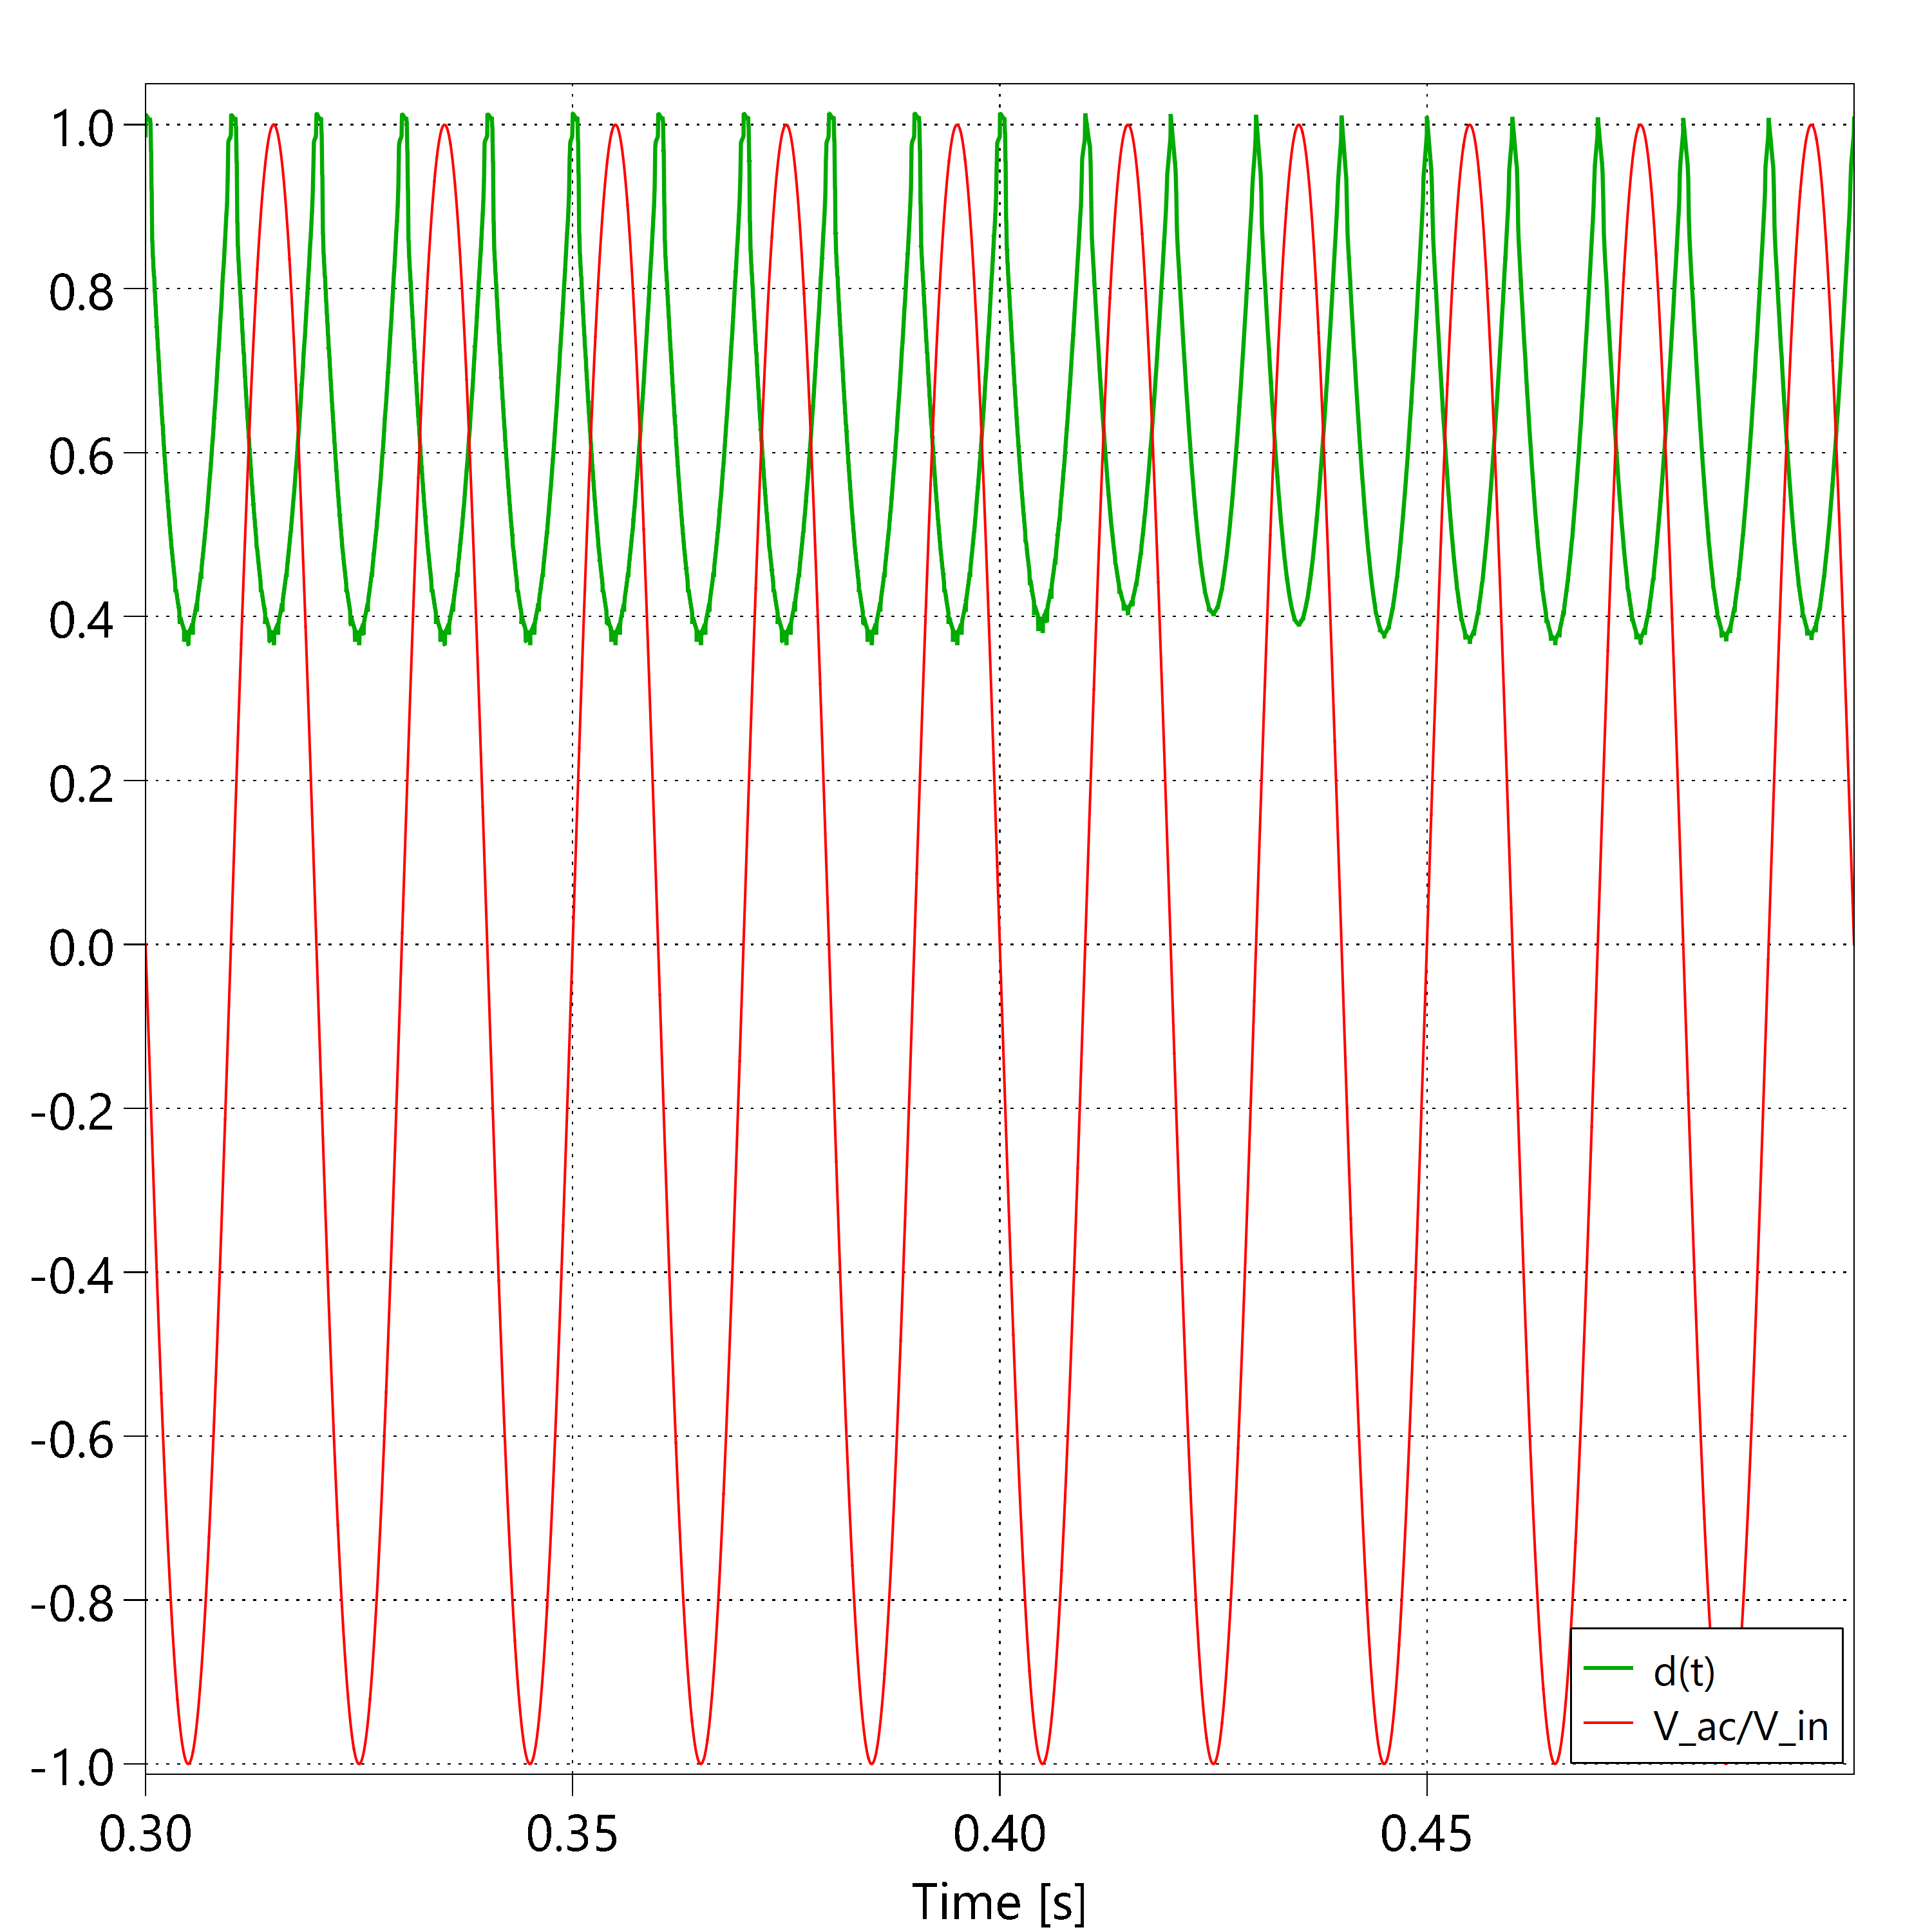
\includegraphics[width=\textwidth]{figures/dutypipr.png} % Replace with your fourth image filename
%         \caption{PI/PR control, Comparison of Duty Cycle vs Normalized Grid Voltage}
%         \label{fig:sub4}
%     \end{subfigure}

    
    
%     % --- Overall Figure Caption and Label ---
%     \caption{Comparative analysis of Lyapunov-based vs. Cascaded PI/PR control strategies.}
%     \label{fig:main}
% \end{figure*}





\begin{figure*}[htbp]
    \centering
    \begin{subfigure}[b]{0.3\textwidth}
        \centering
        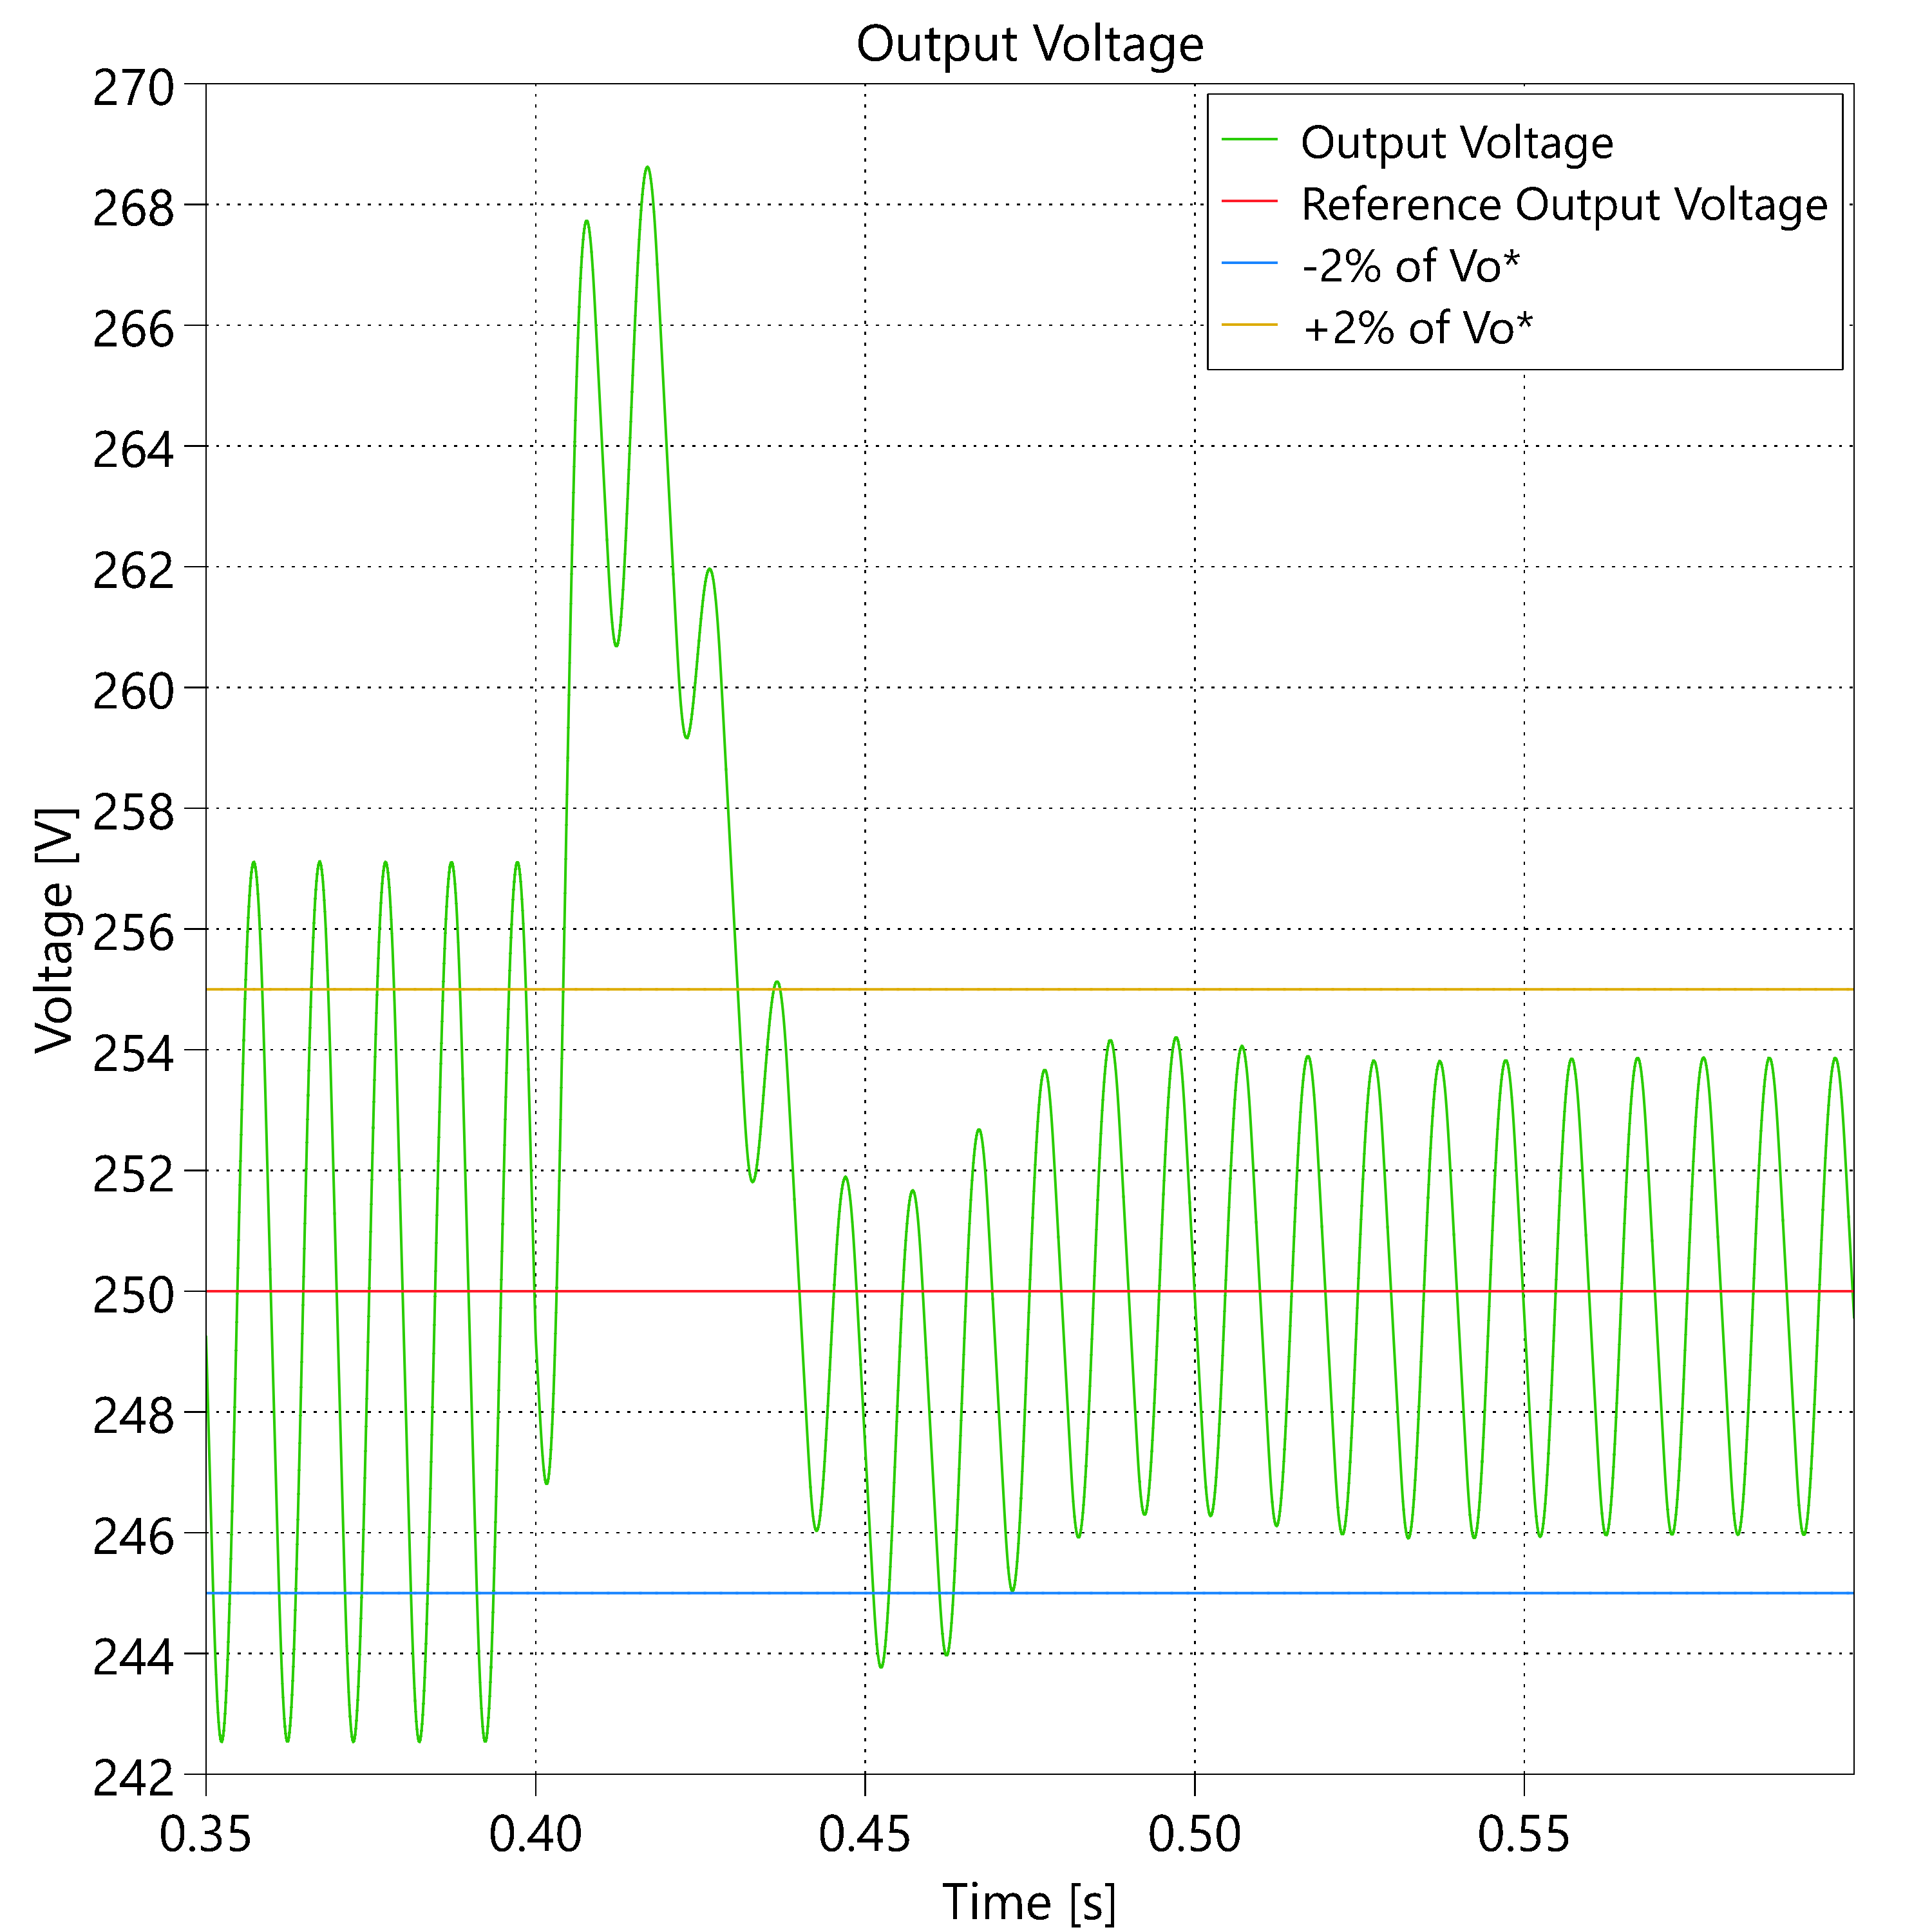
\includegraphics[width=\textwidth]{figures/LYVo1.png}
        \caption{Lyapunov-based Control}
        \label{fig:LYVo1}
    \end{subfigure}% <--- This % kills the hidden space!
    \hfill
    \begin{subfigure}[b]{0.3\textwidth}
        \centering
    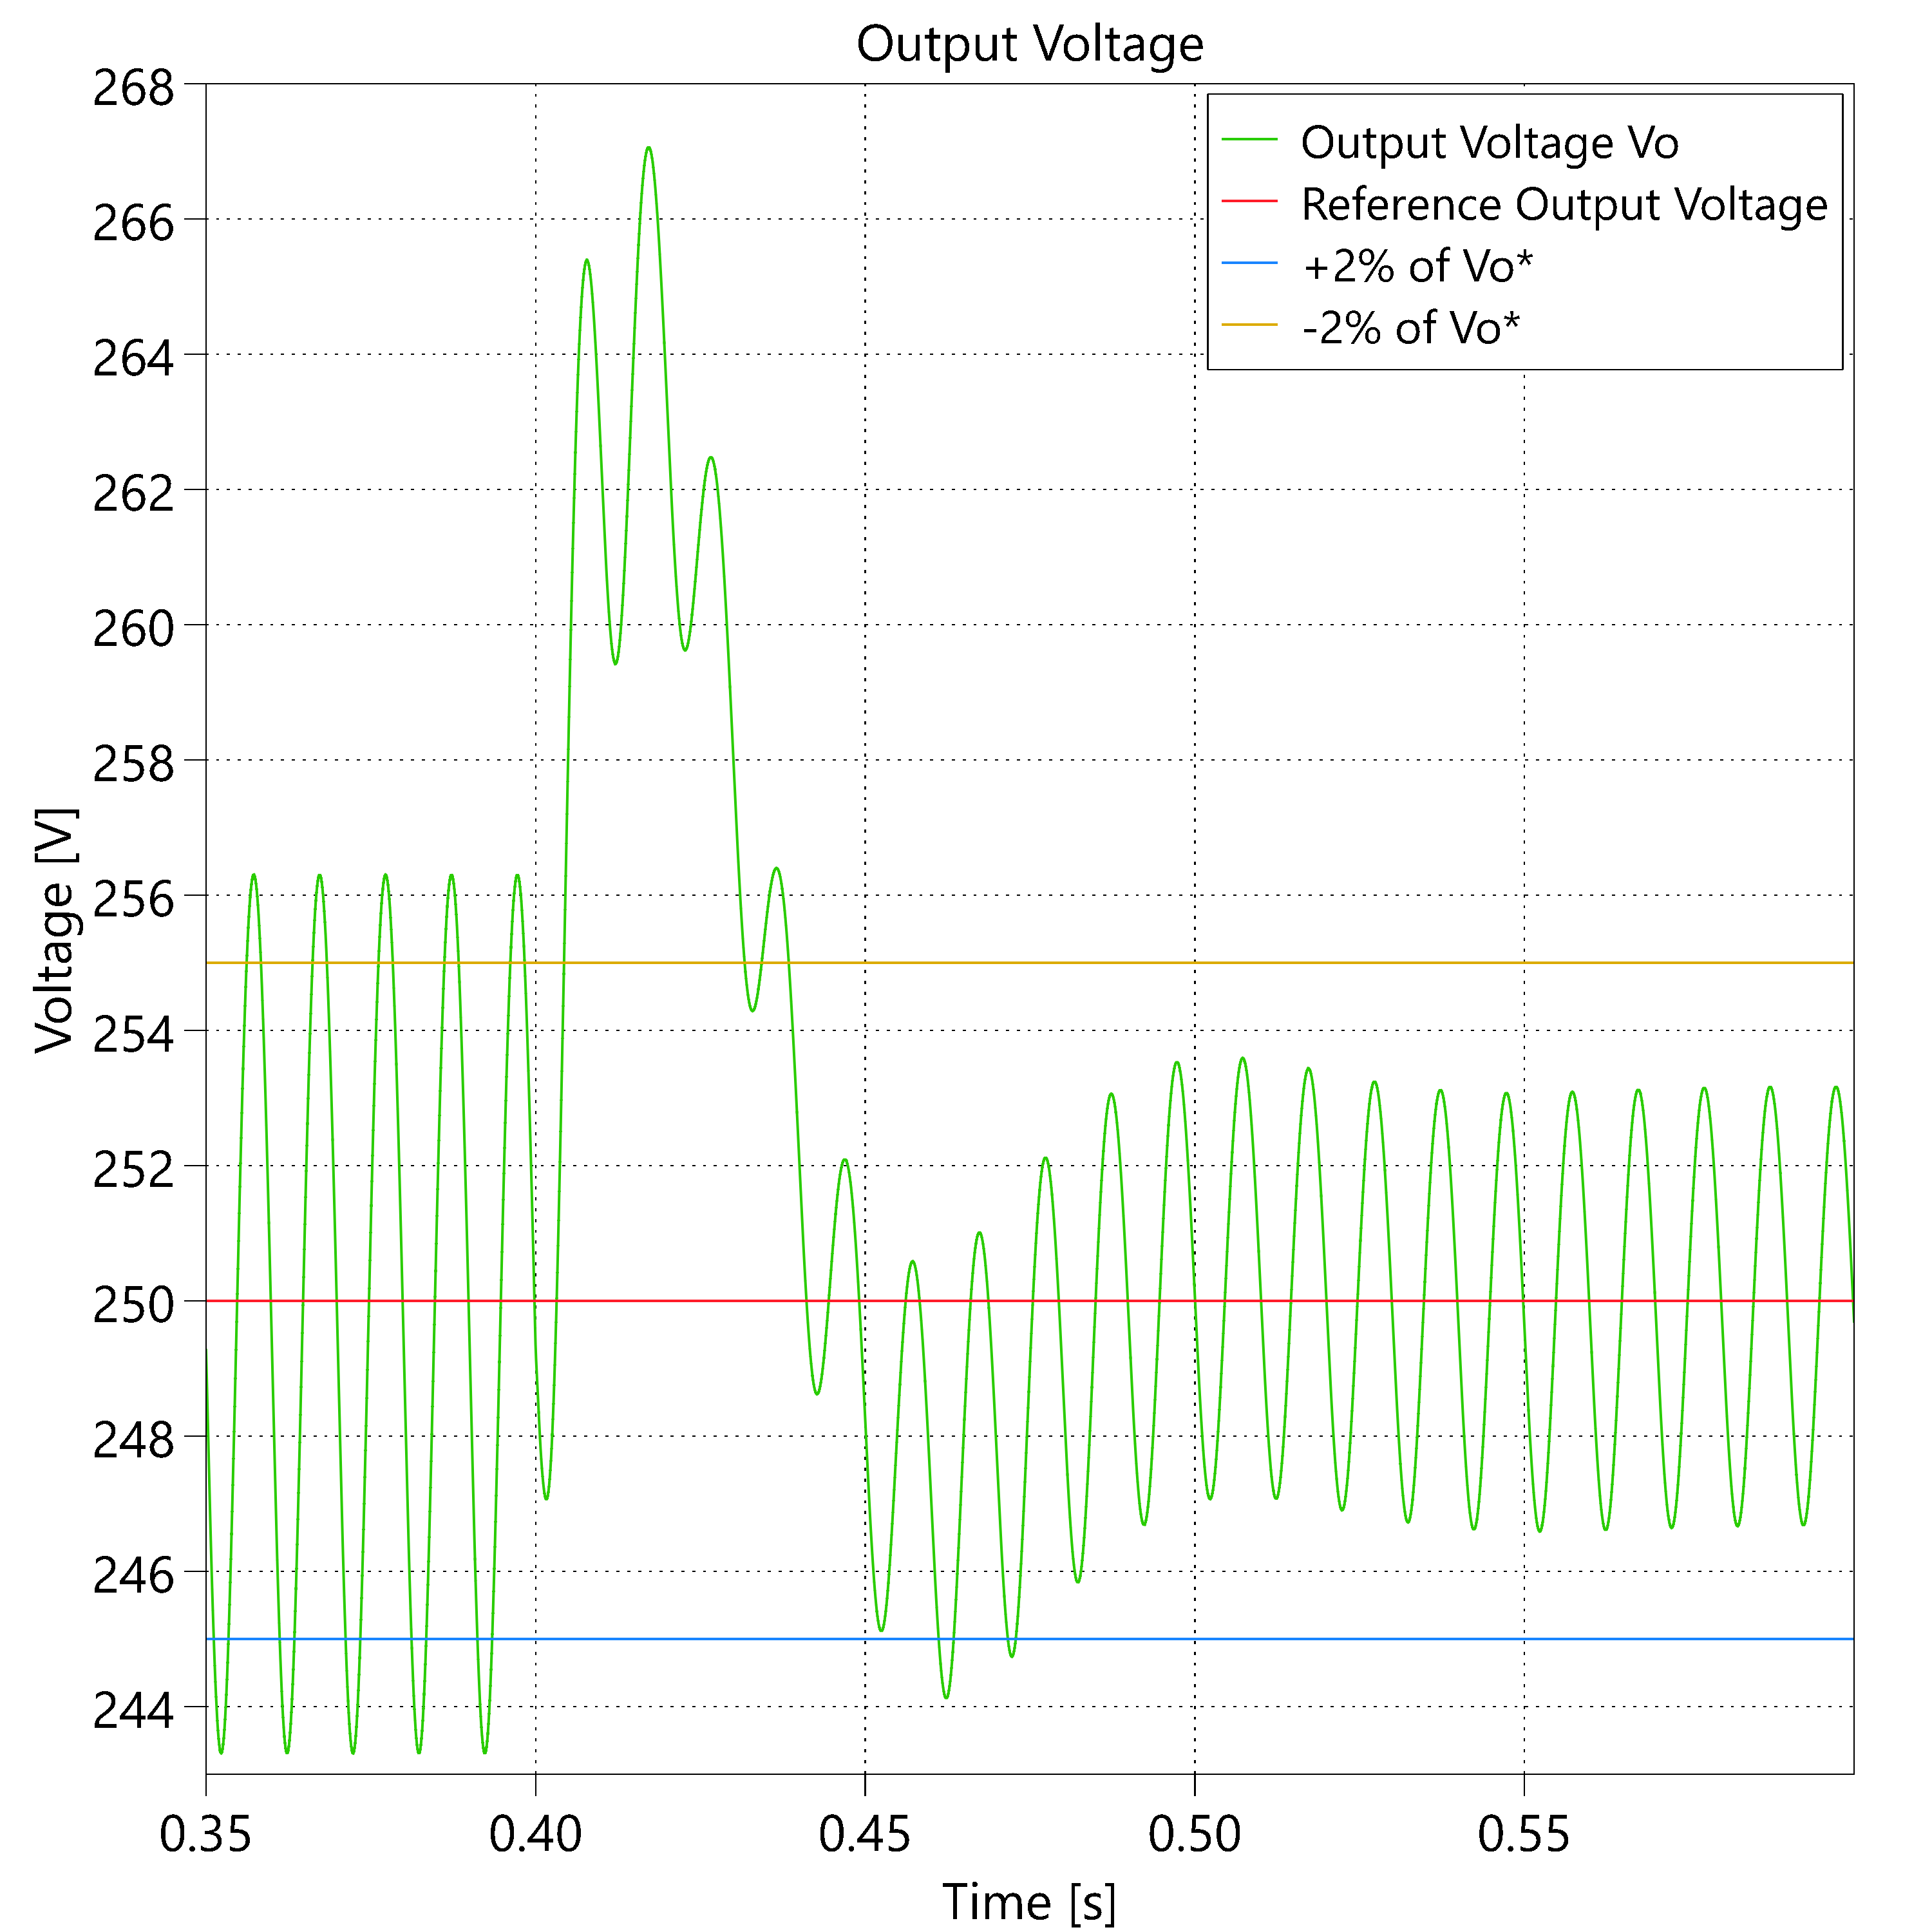
\includegraphics[width=1\linewidth]{figures/piprVO.png}
        \caption{PI/PR Control}
        \label{fig:piprVO}
    \end{subfigure}% <--- This % kills the hidden space!
    \hfill
    \begin{subfigure}[b]{0.3\textwidth}
        \centering
    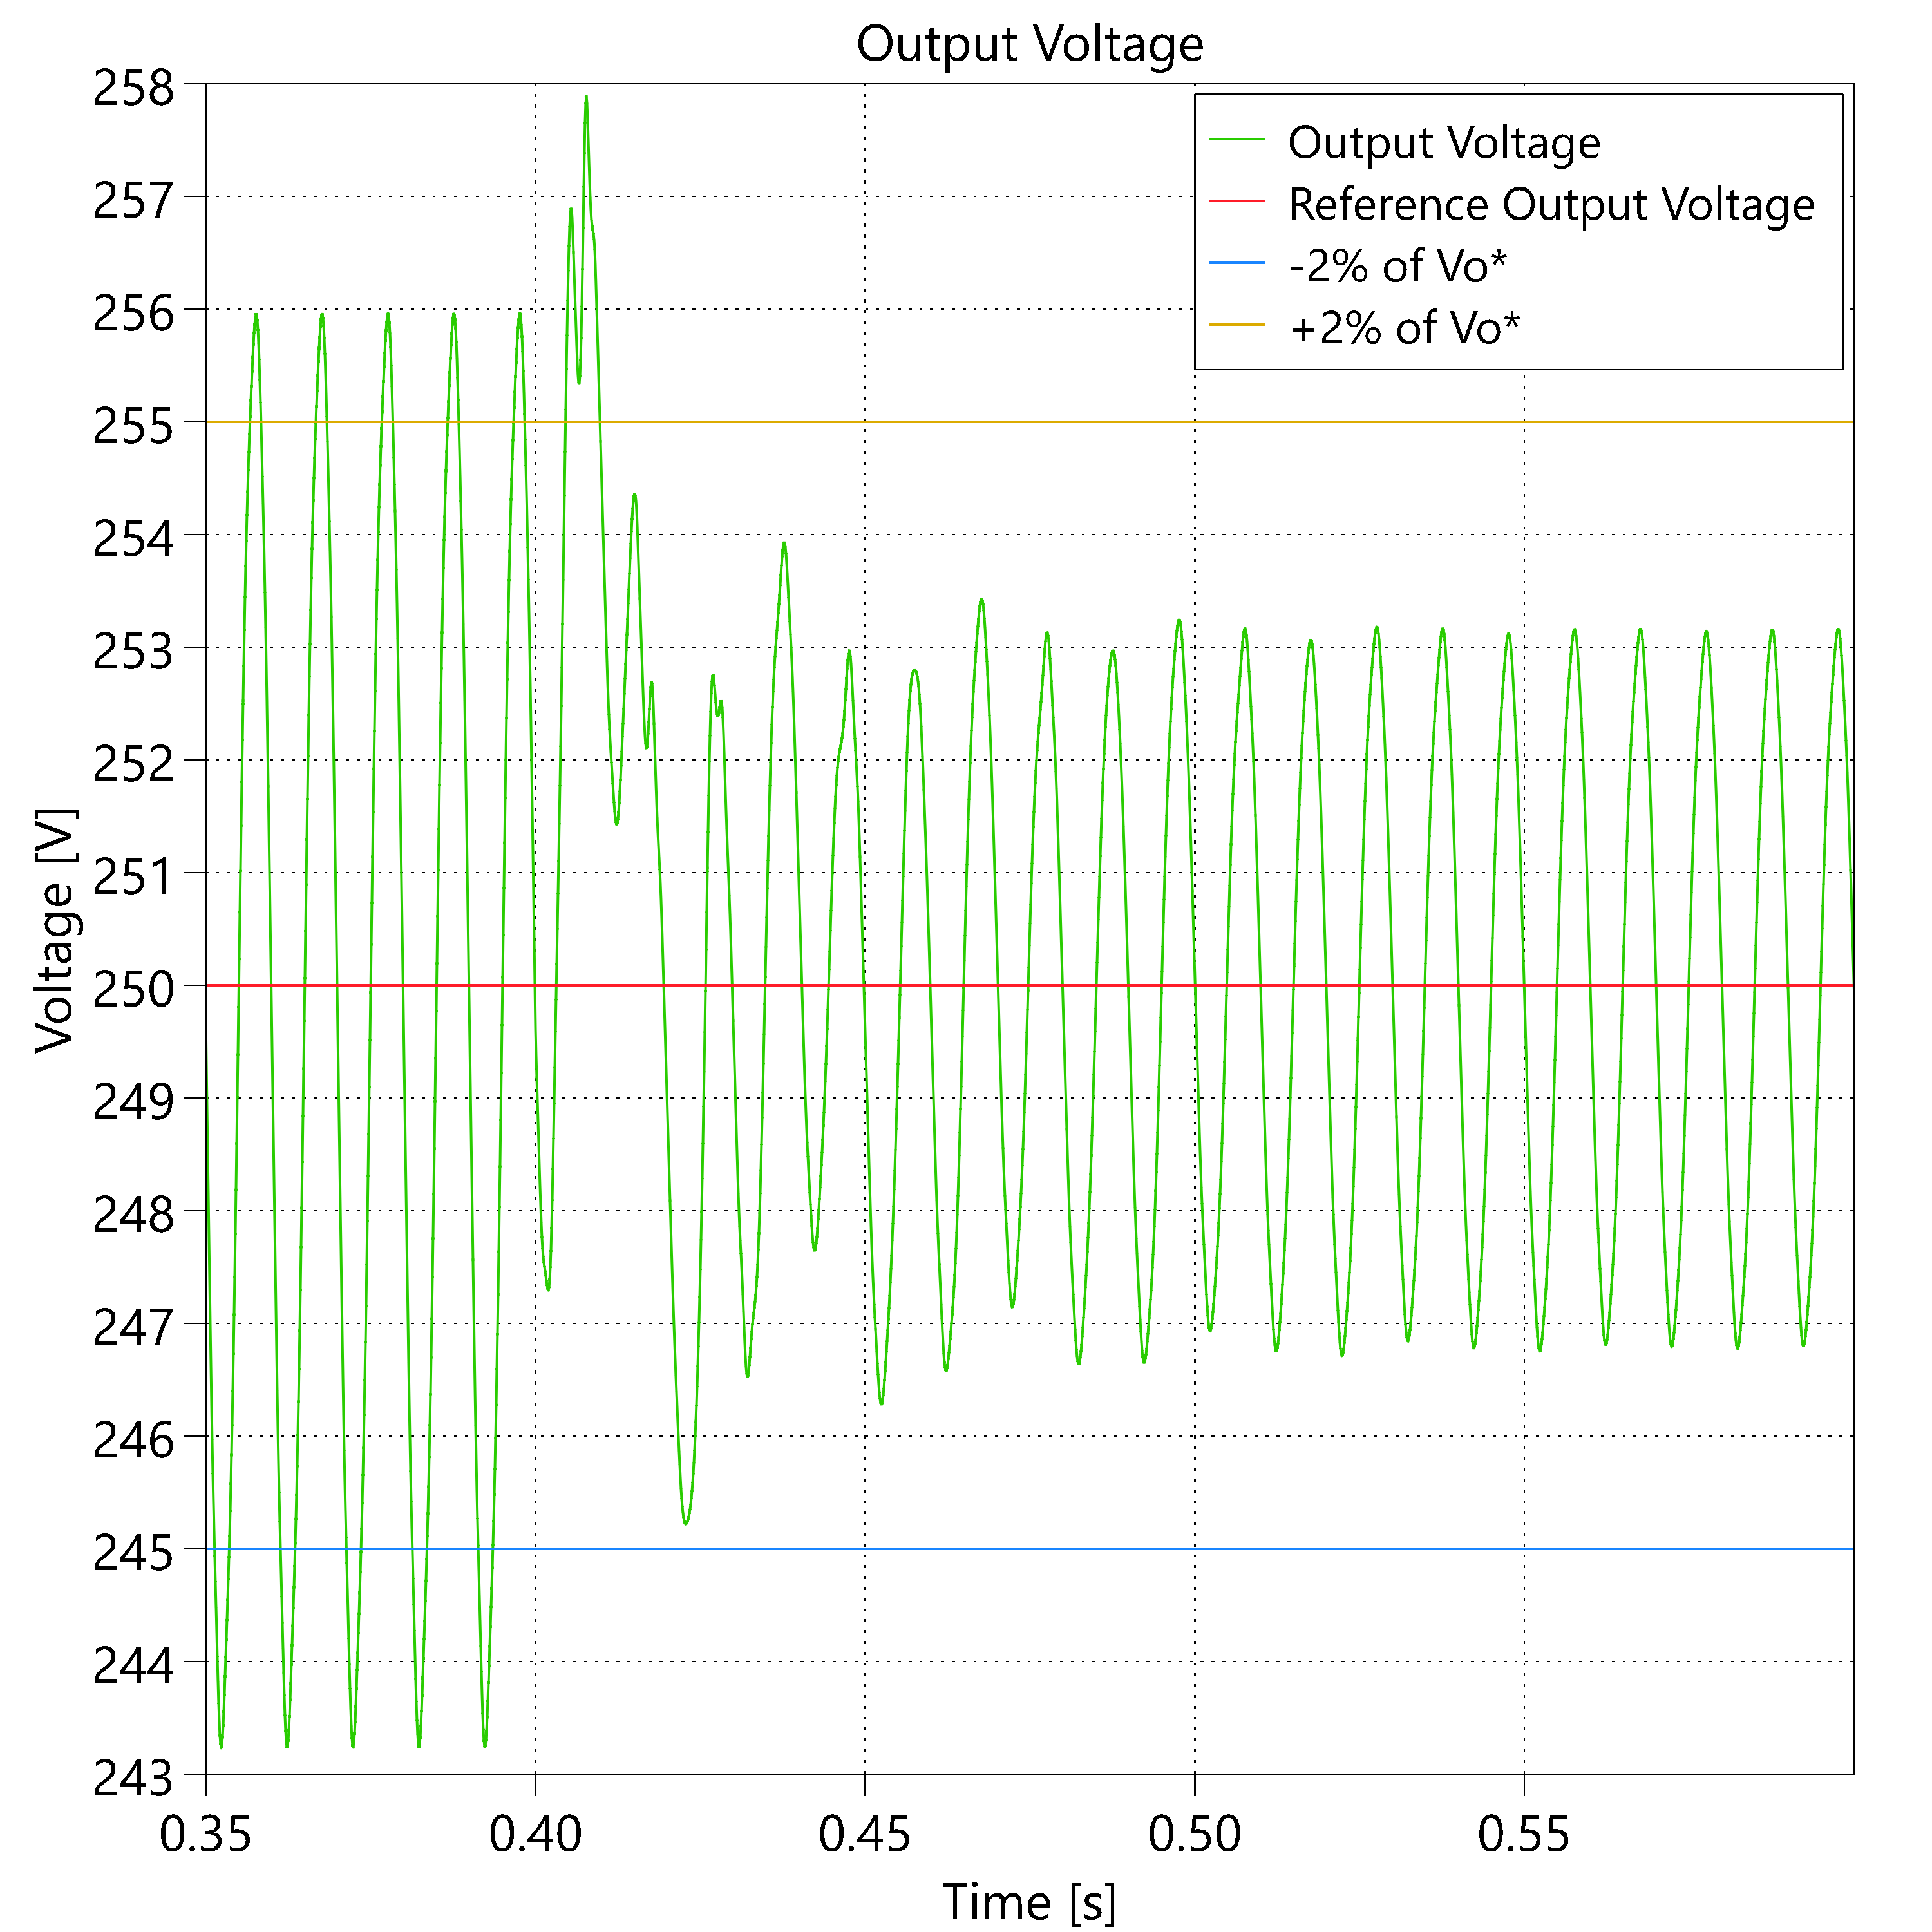
\includegraphics[width=1\linewidth]{figures/Vo_phas_noXa.png}
        \caption{Phasor Domain Control}
        \label{fig:Vo_phas_noXa}
    \end{subfigure}% <--- This % kills the hidden space!
    \caption{Output Voltage simulation results }
    \label{fig:voltage_noXa}
\end{figure*}






The performance of the three models is evaluated through numerical simulations, utilizing the specific parameters detailed in Table \ref{tab:simulation_parameters}. First, a comparative analysis of the control strategies is carrid out without including the feedforward action, $x_{alpha_{ff}}$, focusing on output voltage regulation, the Total Harmonic Distortion (THD) of the inductor current, and the achieved Power Factor (PF). Then, the same analysis is carried out with the feedforward action, and the results obtained are compared with the previous.\\

 To comprehensively characterize the dynamic response of the system, three key parameters are evaluated: the voltage ripple, $\Delta V$, observed both prior to and following the load step at $t=400$ms; the settling time, $t_s$, defined as the duration from $t=400$ms until the waveform permanently enters a $\pm 2 \%$ band around the reference $V^*_o$; and the percentage overshoot, $OS\%$. The performances for each model and relative control strategy are reported in Table \ref{tab:Out_V}.

The resulting output voltage waveforms for the control strategies are illustrated in Fig. \ref{fig:voltage_noXa}.
The two control strategies operating in the stationary reference frame yield similar output voltage results, as can be seen in Fig. \ref{fig:LYVo1} and \ref{fig:piprVO}, respectively, for the Lyapunov-based and PI/PR controls. The Lyapunov controllers present a smaller ripple and settling time, as we can see in Table \ref{tab:Out_V}.
The difference is in the THD, where the Lyapunov controller produces a higher distortion.
Both the PI/PR and Lyapunov controllers demonstrate comparable, standard steady-state ripple characteristics, hovering around 7.2V to 7.6V at $125 \Omega$ and 4.2V to 4.3V at $250 \Omega$. In terms of steady-state performance, the Phasor Domain Control yields the lowest voltage ripple under both load conditions. The Phasor Domain Control obtains a settling time of just 10ms and an overshoot of $3.15\%$, and it rejects the load disturbance almost instantaneously. The corresponding waveform confirms that the voltage recovers immediately after the load step. It can be noted that the overall voltage regulation is much better than the control strategies in the stationary reference frame, as shown in Fig. \ref{fig:Vo_phas_noXa}.


\begin{table}[htp]
    \centering
    \caption{Output Voltage Performance Parameters}
    \label{tab:Out_V}
    \pgfplotstabletypeset[normal,
        columns/Parameter/.style={column name={\textbf{Parameter}}},
        columns/Value/.style={column name={\textbf{Value}}}
    ]{ %
    Parameter         & Value \\
    \topmidheader{2}{Lyapunov Control ($K_c = 0.002$)}
    {Ripple, $\Delta V$}          & {$7.1V\space@\space R_o = 125\Omega; 3.8 V \space @\space R_o = 250\Omega$} \\
    {Settling Time, $t_s$}   & {$64$ ms} \\
    {Overshoot, $OS\%$}       & {$7.2\%$} \\
    \midheader{2}{PI/PR Control}
    {Ripple, $\Delta V$}          & {$7.6V\space@\space R_o =125\Omega; 4.2V\space@\space R_o =250\Omega$} \\ 
    {Settling Time, $t_s$}   & {$82$ ms} \\ 
    {Overshoot, $OS\%$}       & {$6.4\%$} \\
    \midheader{2}{Phasor Domain Control}
    {Ripple, $\Delta V$}          & {$5.6V\space@\space R_o =125\Omega; 3.2V\space@\space R_o =250\Omega$} \\ 
    {Settling Time, $t_s$}   & {$10$ ms} \\ 
    {Overshoot, $OS\%$}       & {$3.15\%$} \\
    }
\end{table}

\begin{figure}[htp]
    \centering
    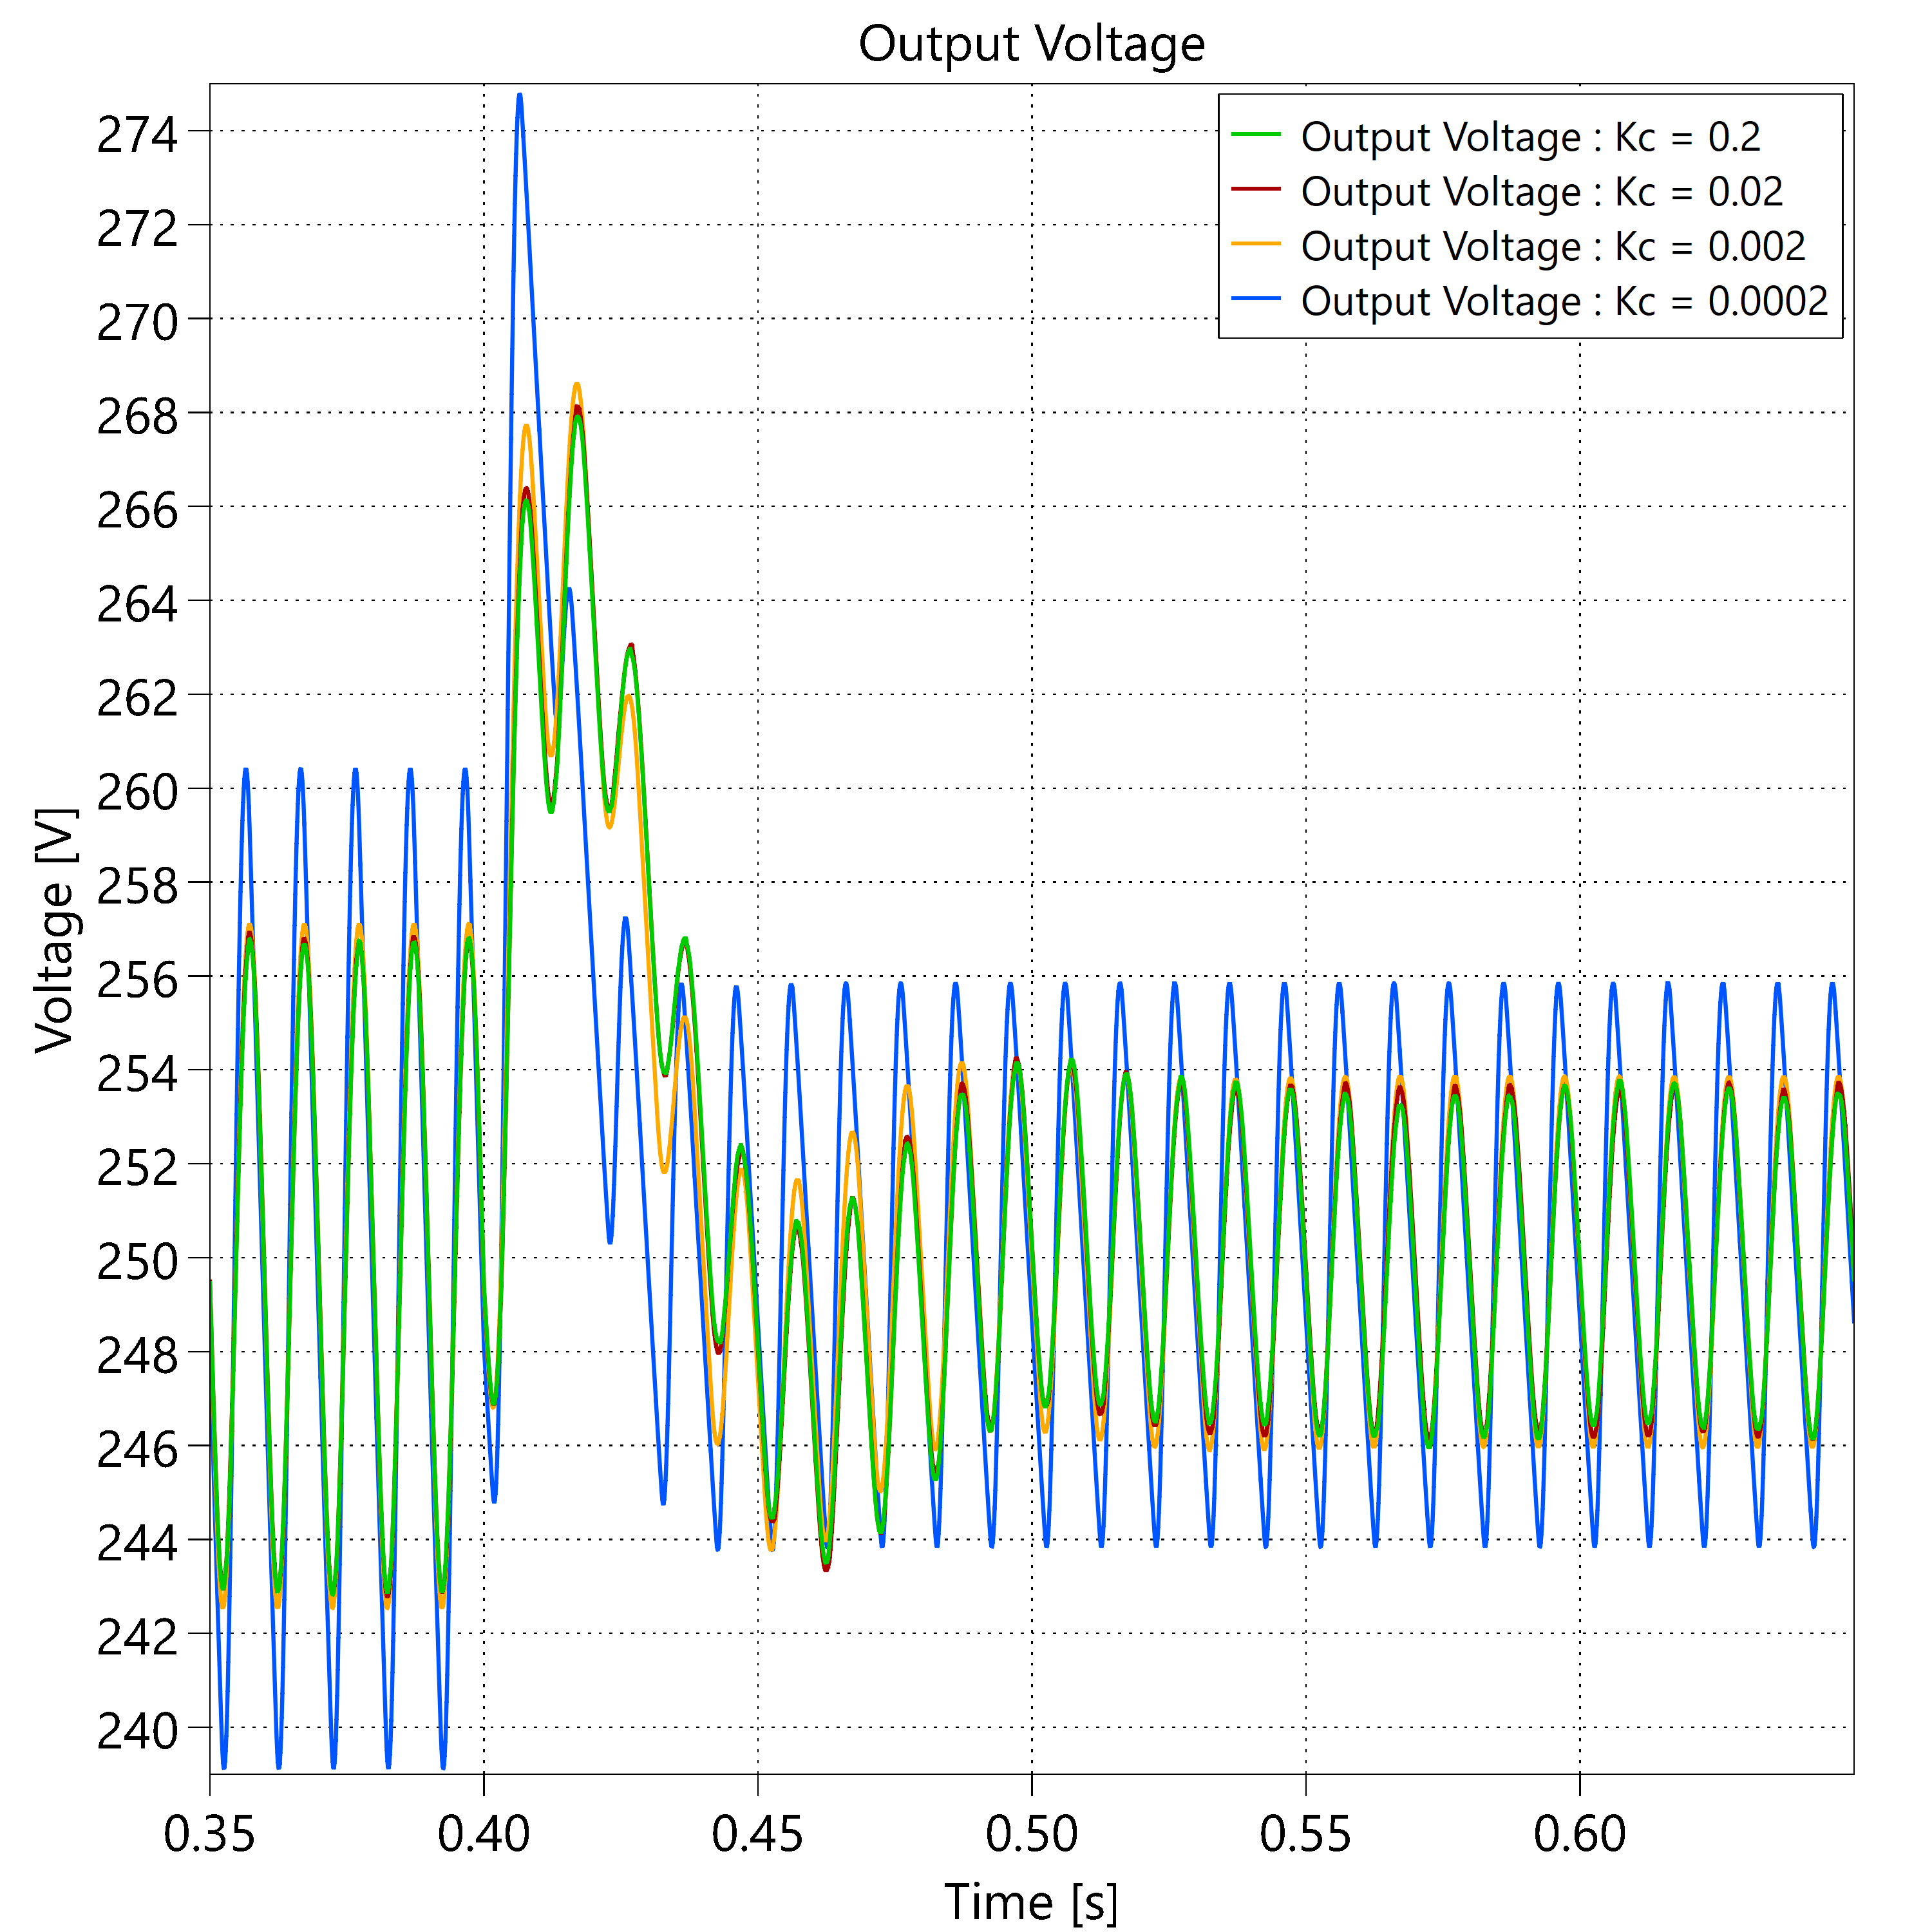
\includegraphics[width=0.8\linewidth]{figures/LY_vo_kc.png}
    \caption{Output Voltage Regulation of Lyapunov controller with different $K_c$ values }
    \label{fig:LY_vo_kc}
\end{figure}
\begin{figure}[htp]
    \centering
    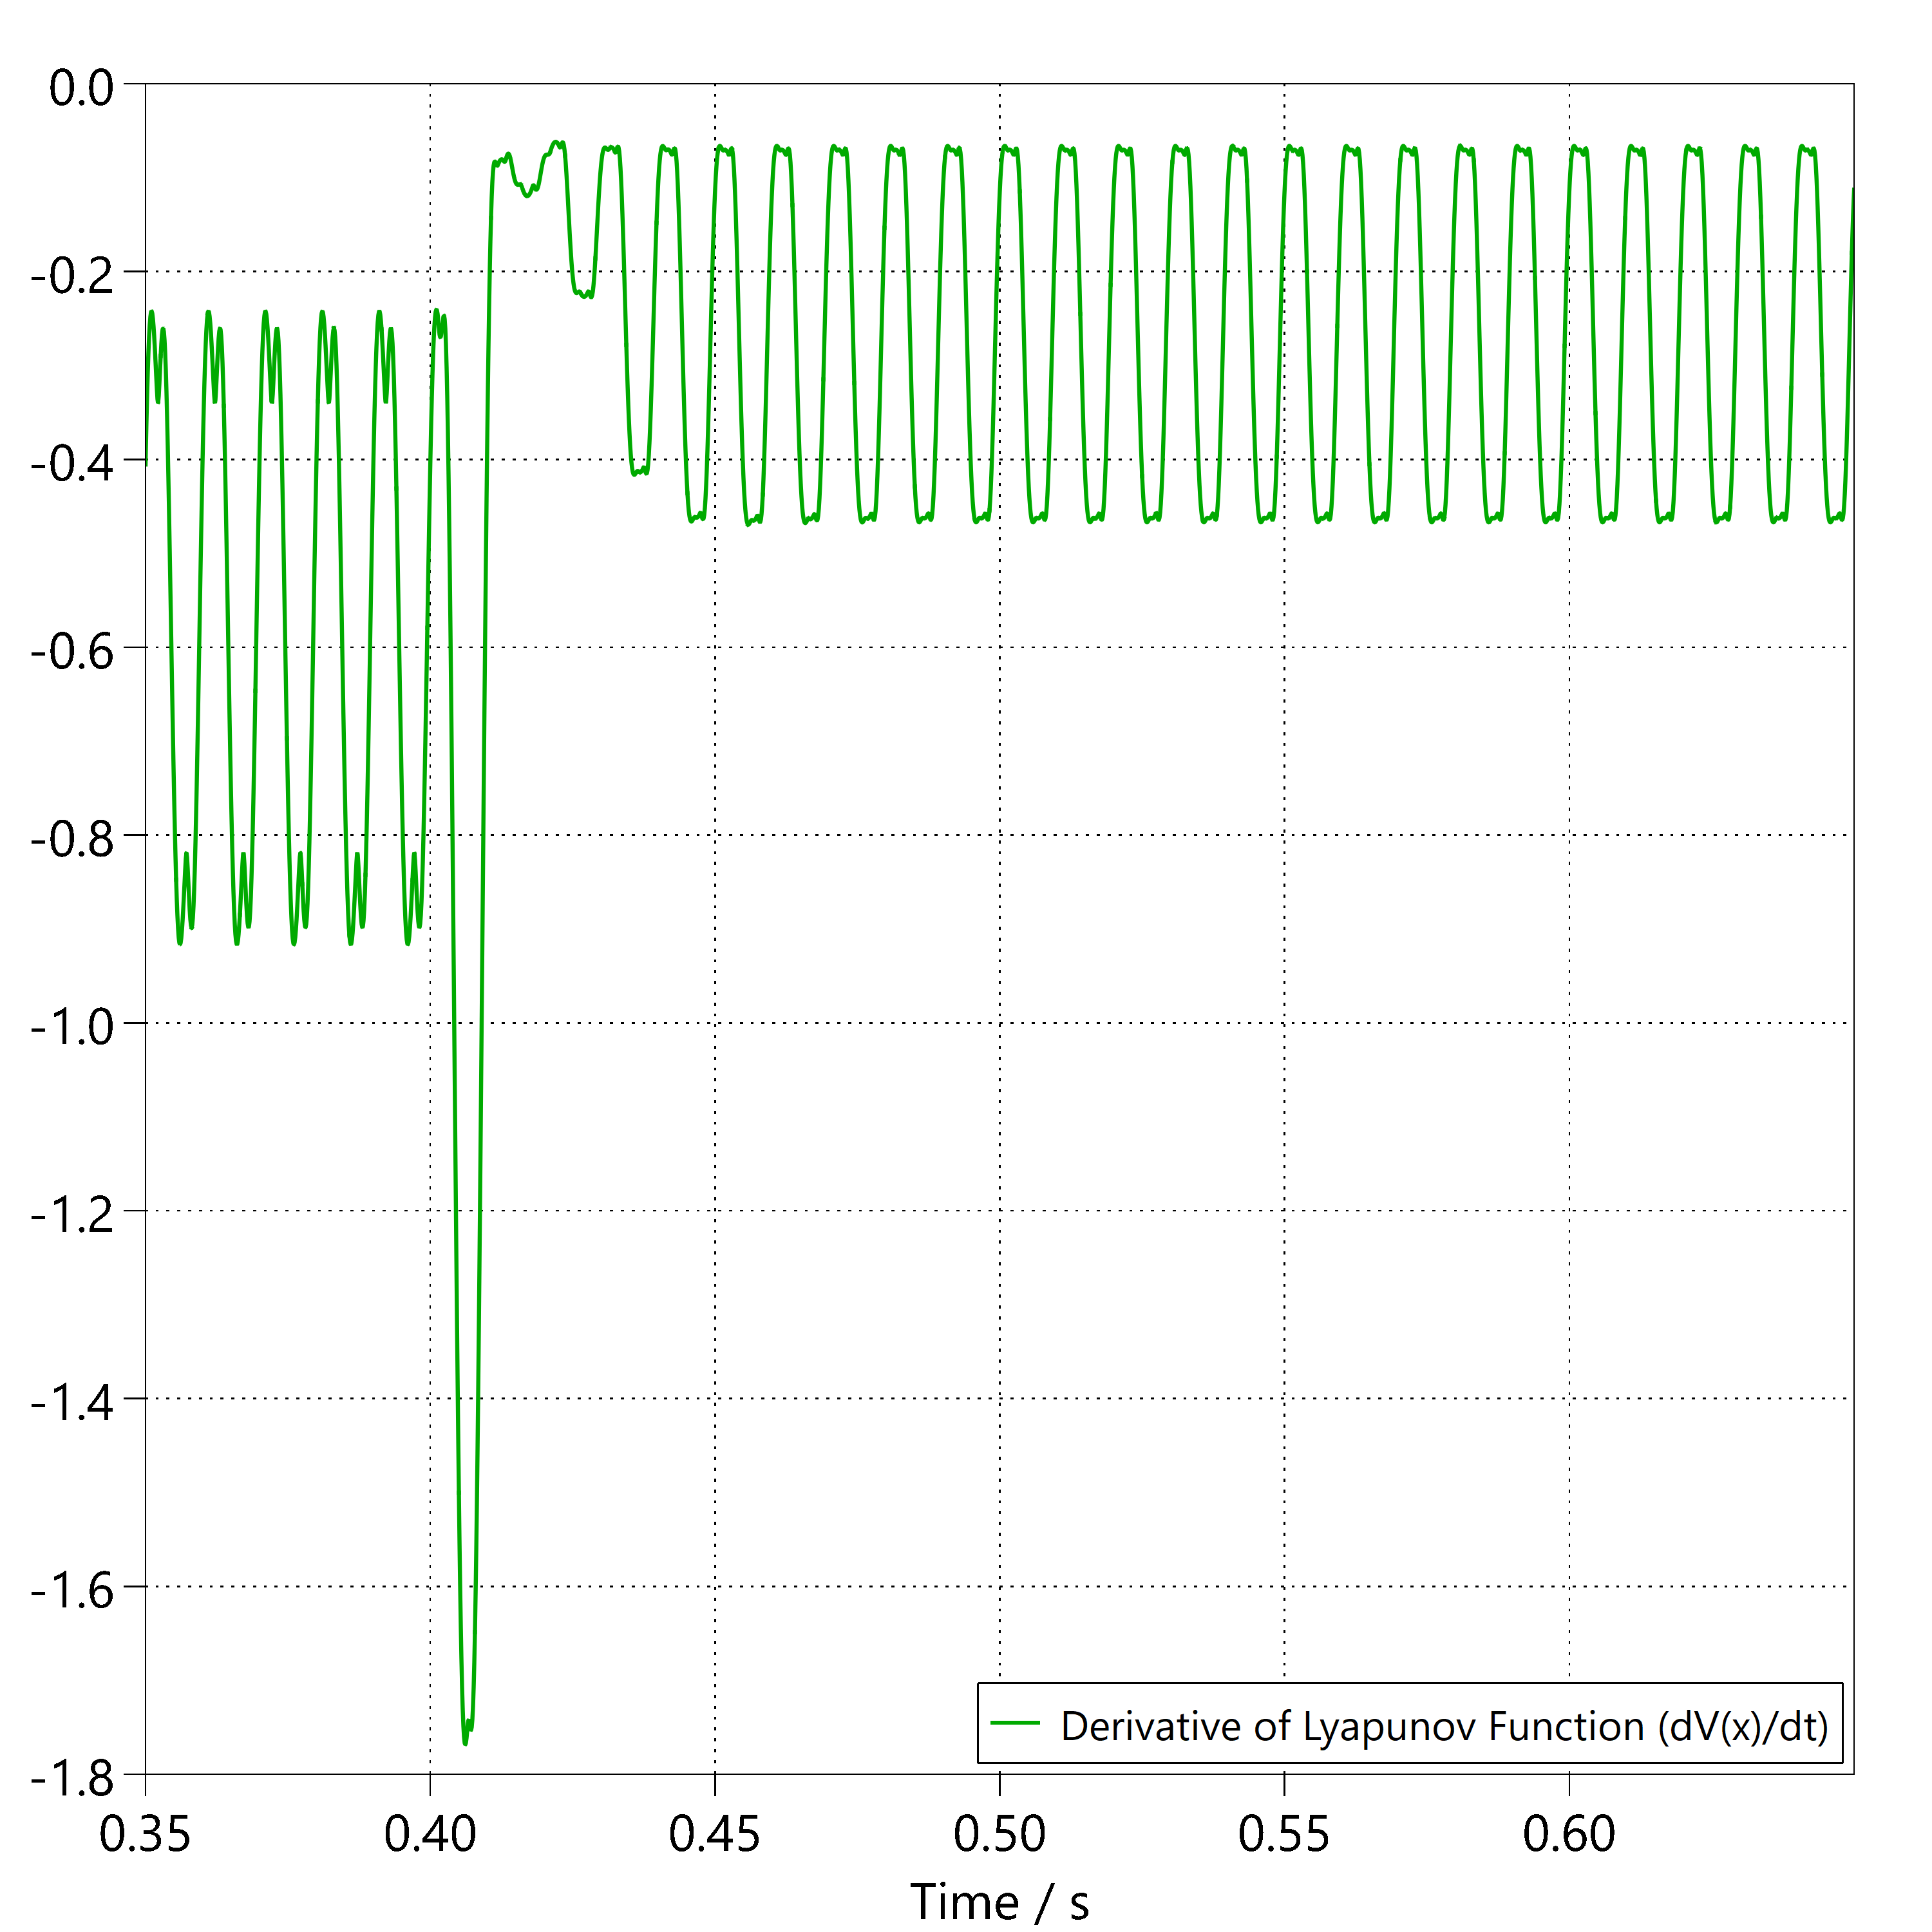
\includegraphics[width=0.8\linewidth]{figures/dV_dt_LY.png}
    \caption{Derivative of Lyapunov Function}
    \label{fig:dV_dt_LY}
\end{figure}
The effects on the voltage regulation of different values for the proportional gain $K_c$ used in (\ref{eq:LY_control}) have been investigated, and the results are shown in Fig. \ref{fig:LY_vo_kc}. Increasing the value of $K_c$ from $0.0002$ to $0.2$ yields an increasing power factor, and thus a lower THD, at the cost of a nosier duty cycle. Further, for large values of $K_c$, such $K_c = 0.2$, the settling time tends to increase, but the overshoot decreases. For smaller values of $K_c$, such as $K_c = 0.0002$, the overshoot increases. Further, for such small values, the output voltage never settles within the $\pm 2\%$ band of the reference output voltage $V^*_o$. Thus, while global asymptotic stability is guaranteed in general, as demonstrated in Fig. \ref{fig:dV_dt_LY}, the performance of the Lyapunov-based controller heavily depend on the value of the gain $K_c$. These results are summarized in Table \ref{tab:Lyapunov_Transient}.
\begin{figure*}[htbp]
    \centering
    \begin{subfigure}[b]{0.3\textwidth}
        \centering
        
\includegraphics[width=\textwidth]{figures/Inductor_Current_VS_Input_Voltage_Lyapunov_controller.png}
        \caption{Lyapunov-based Control}
        \label{fig:LY_Ind_curr}
    \end{subfigure}% <--- This % kills the hidden space!
    \hfill
    \begin{subfigure}[b]{0.3\textwidth}
        \centering
    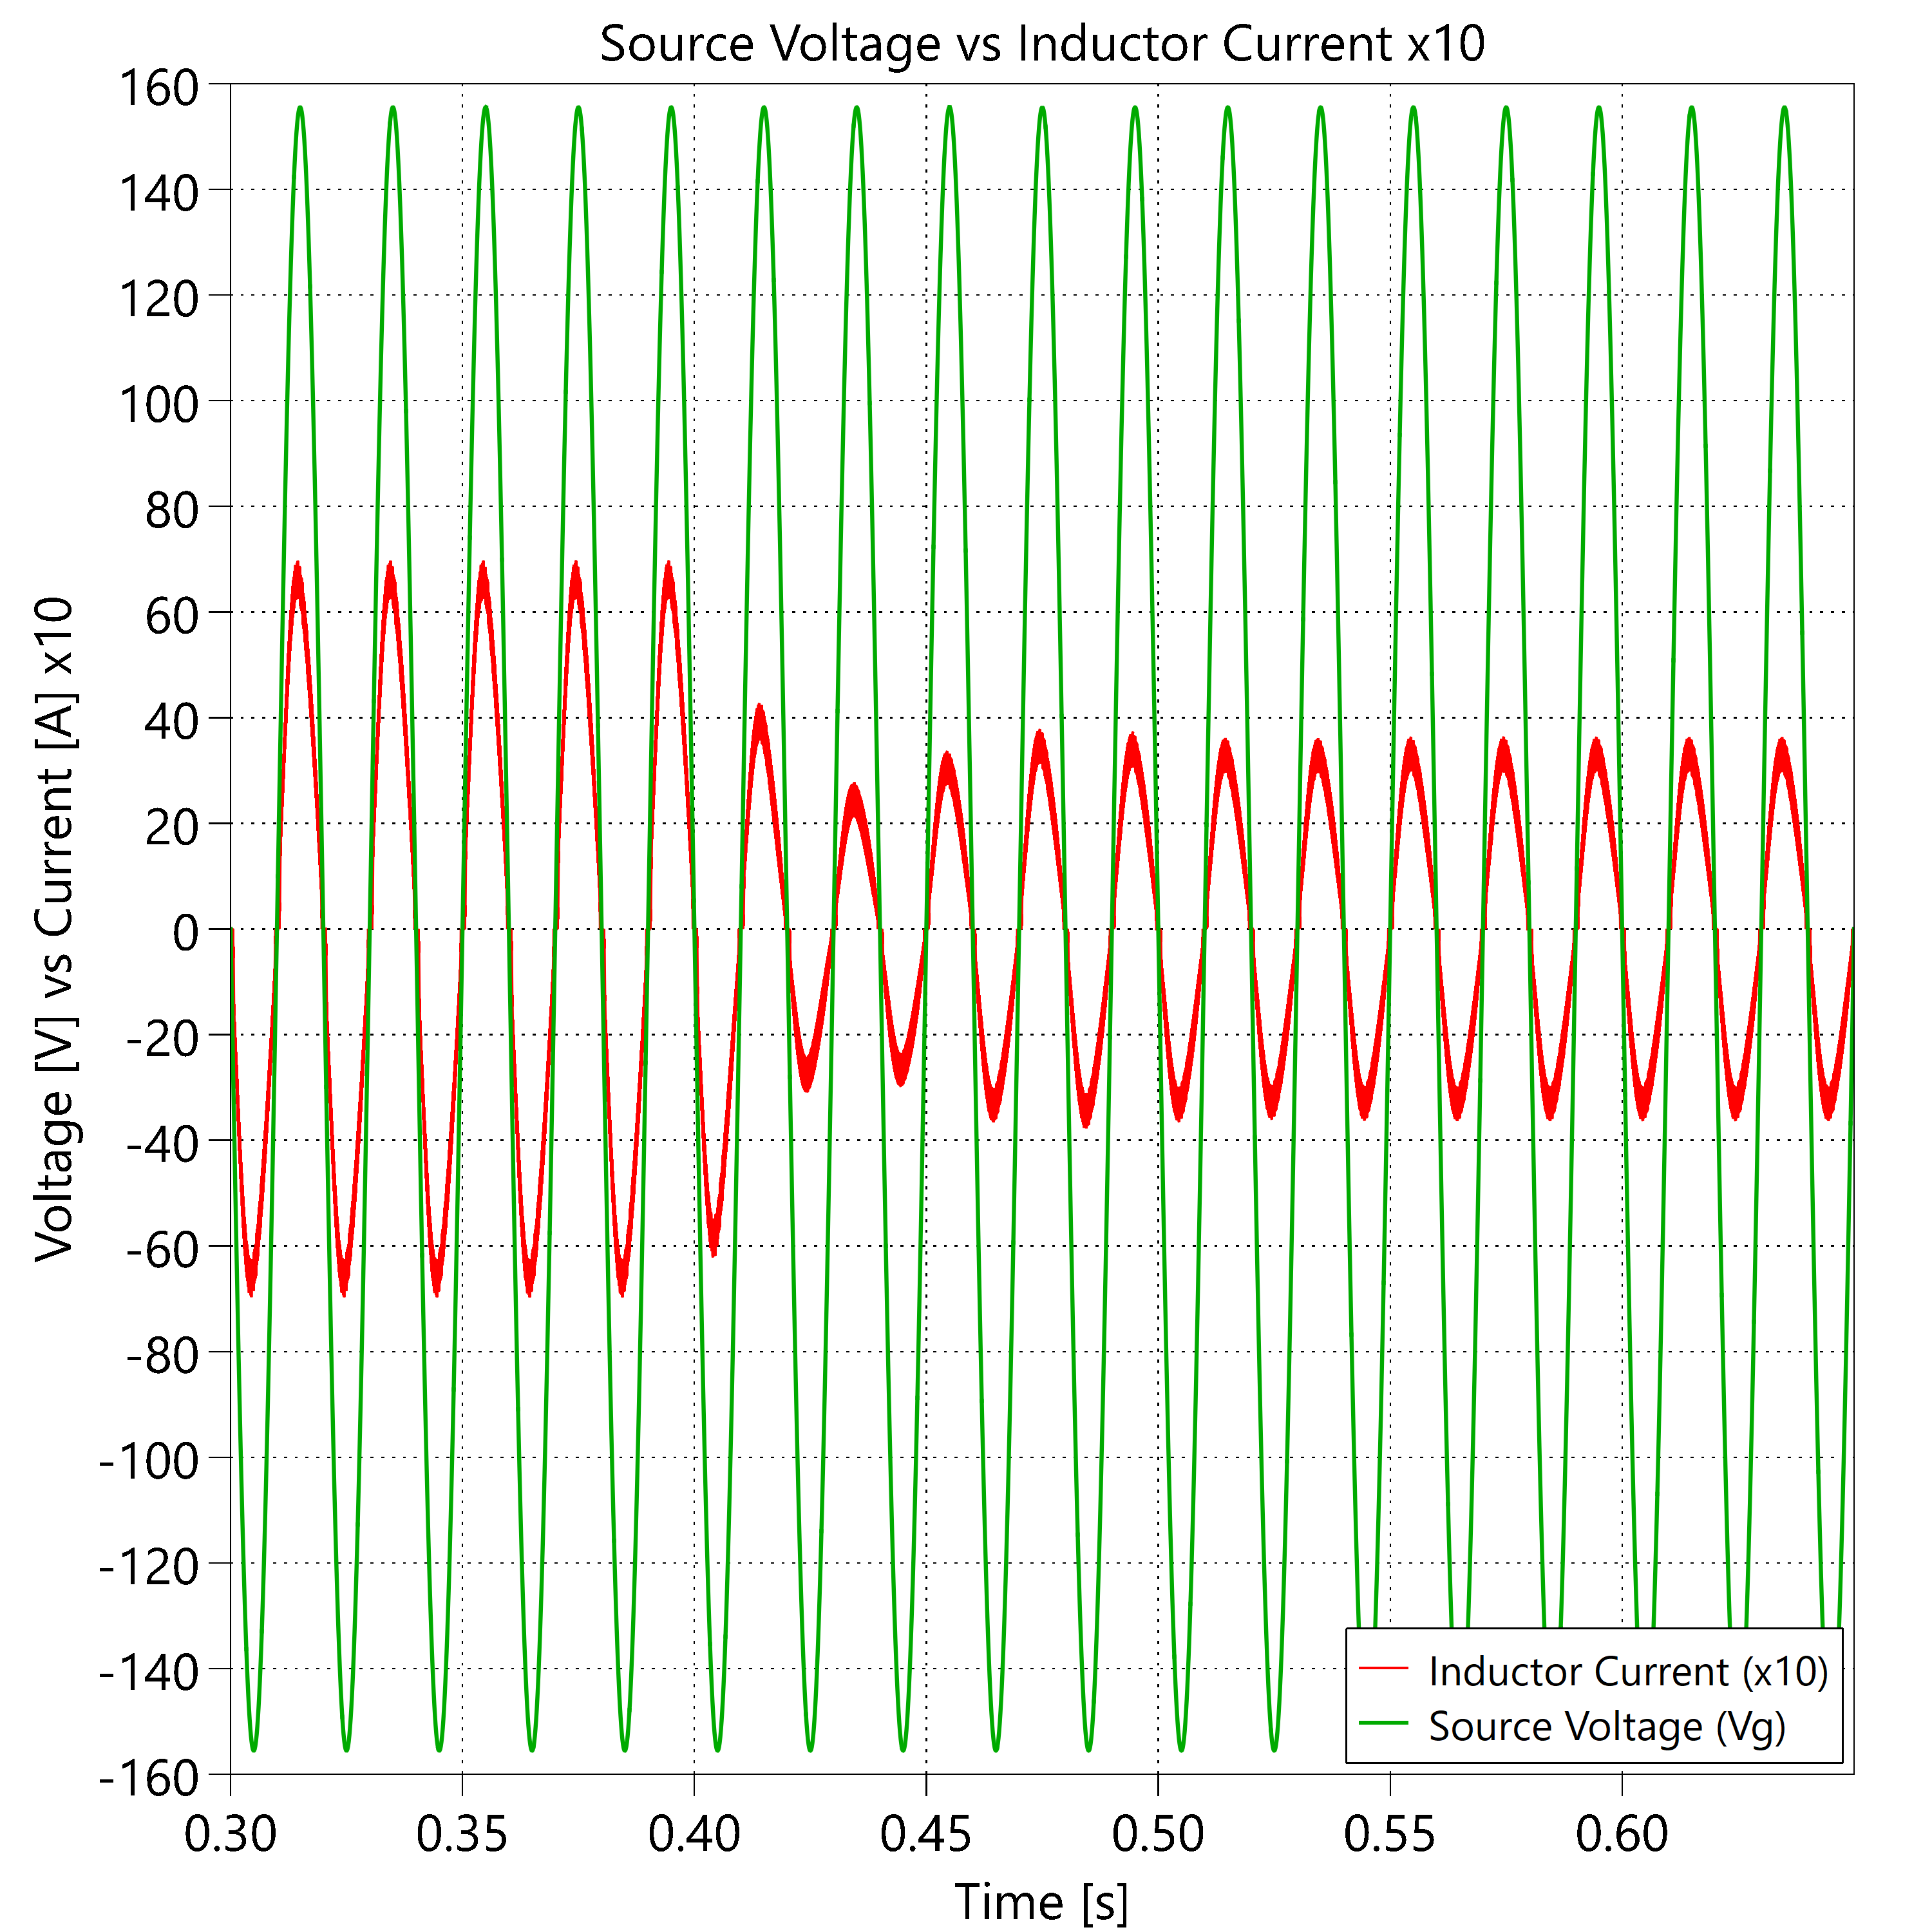
\includegraphics[width=1\linewidth]{figures/pipriAC.png}
        \caption{PI/PR Control}
        \label{fig:PI_PR_Ind_curr}
    \end{subfigure}% <--- This % kills the hidden space!
    \hfill
    \begin{subfigure}[b]{0.3\textwidth}
        \centering
    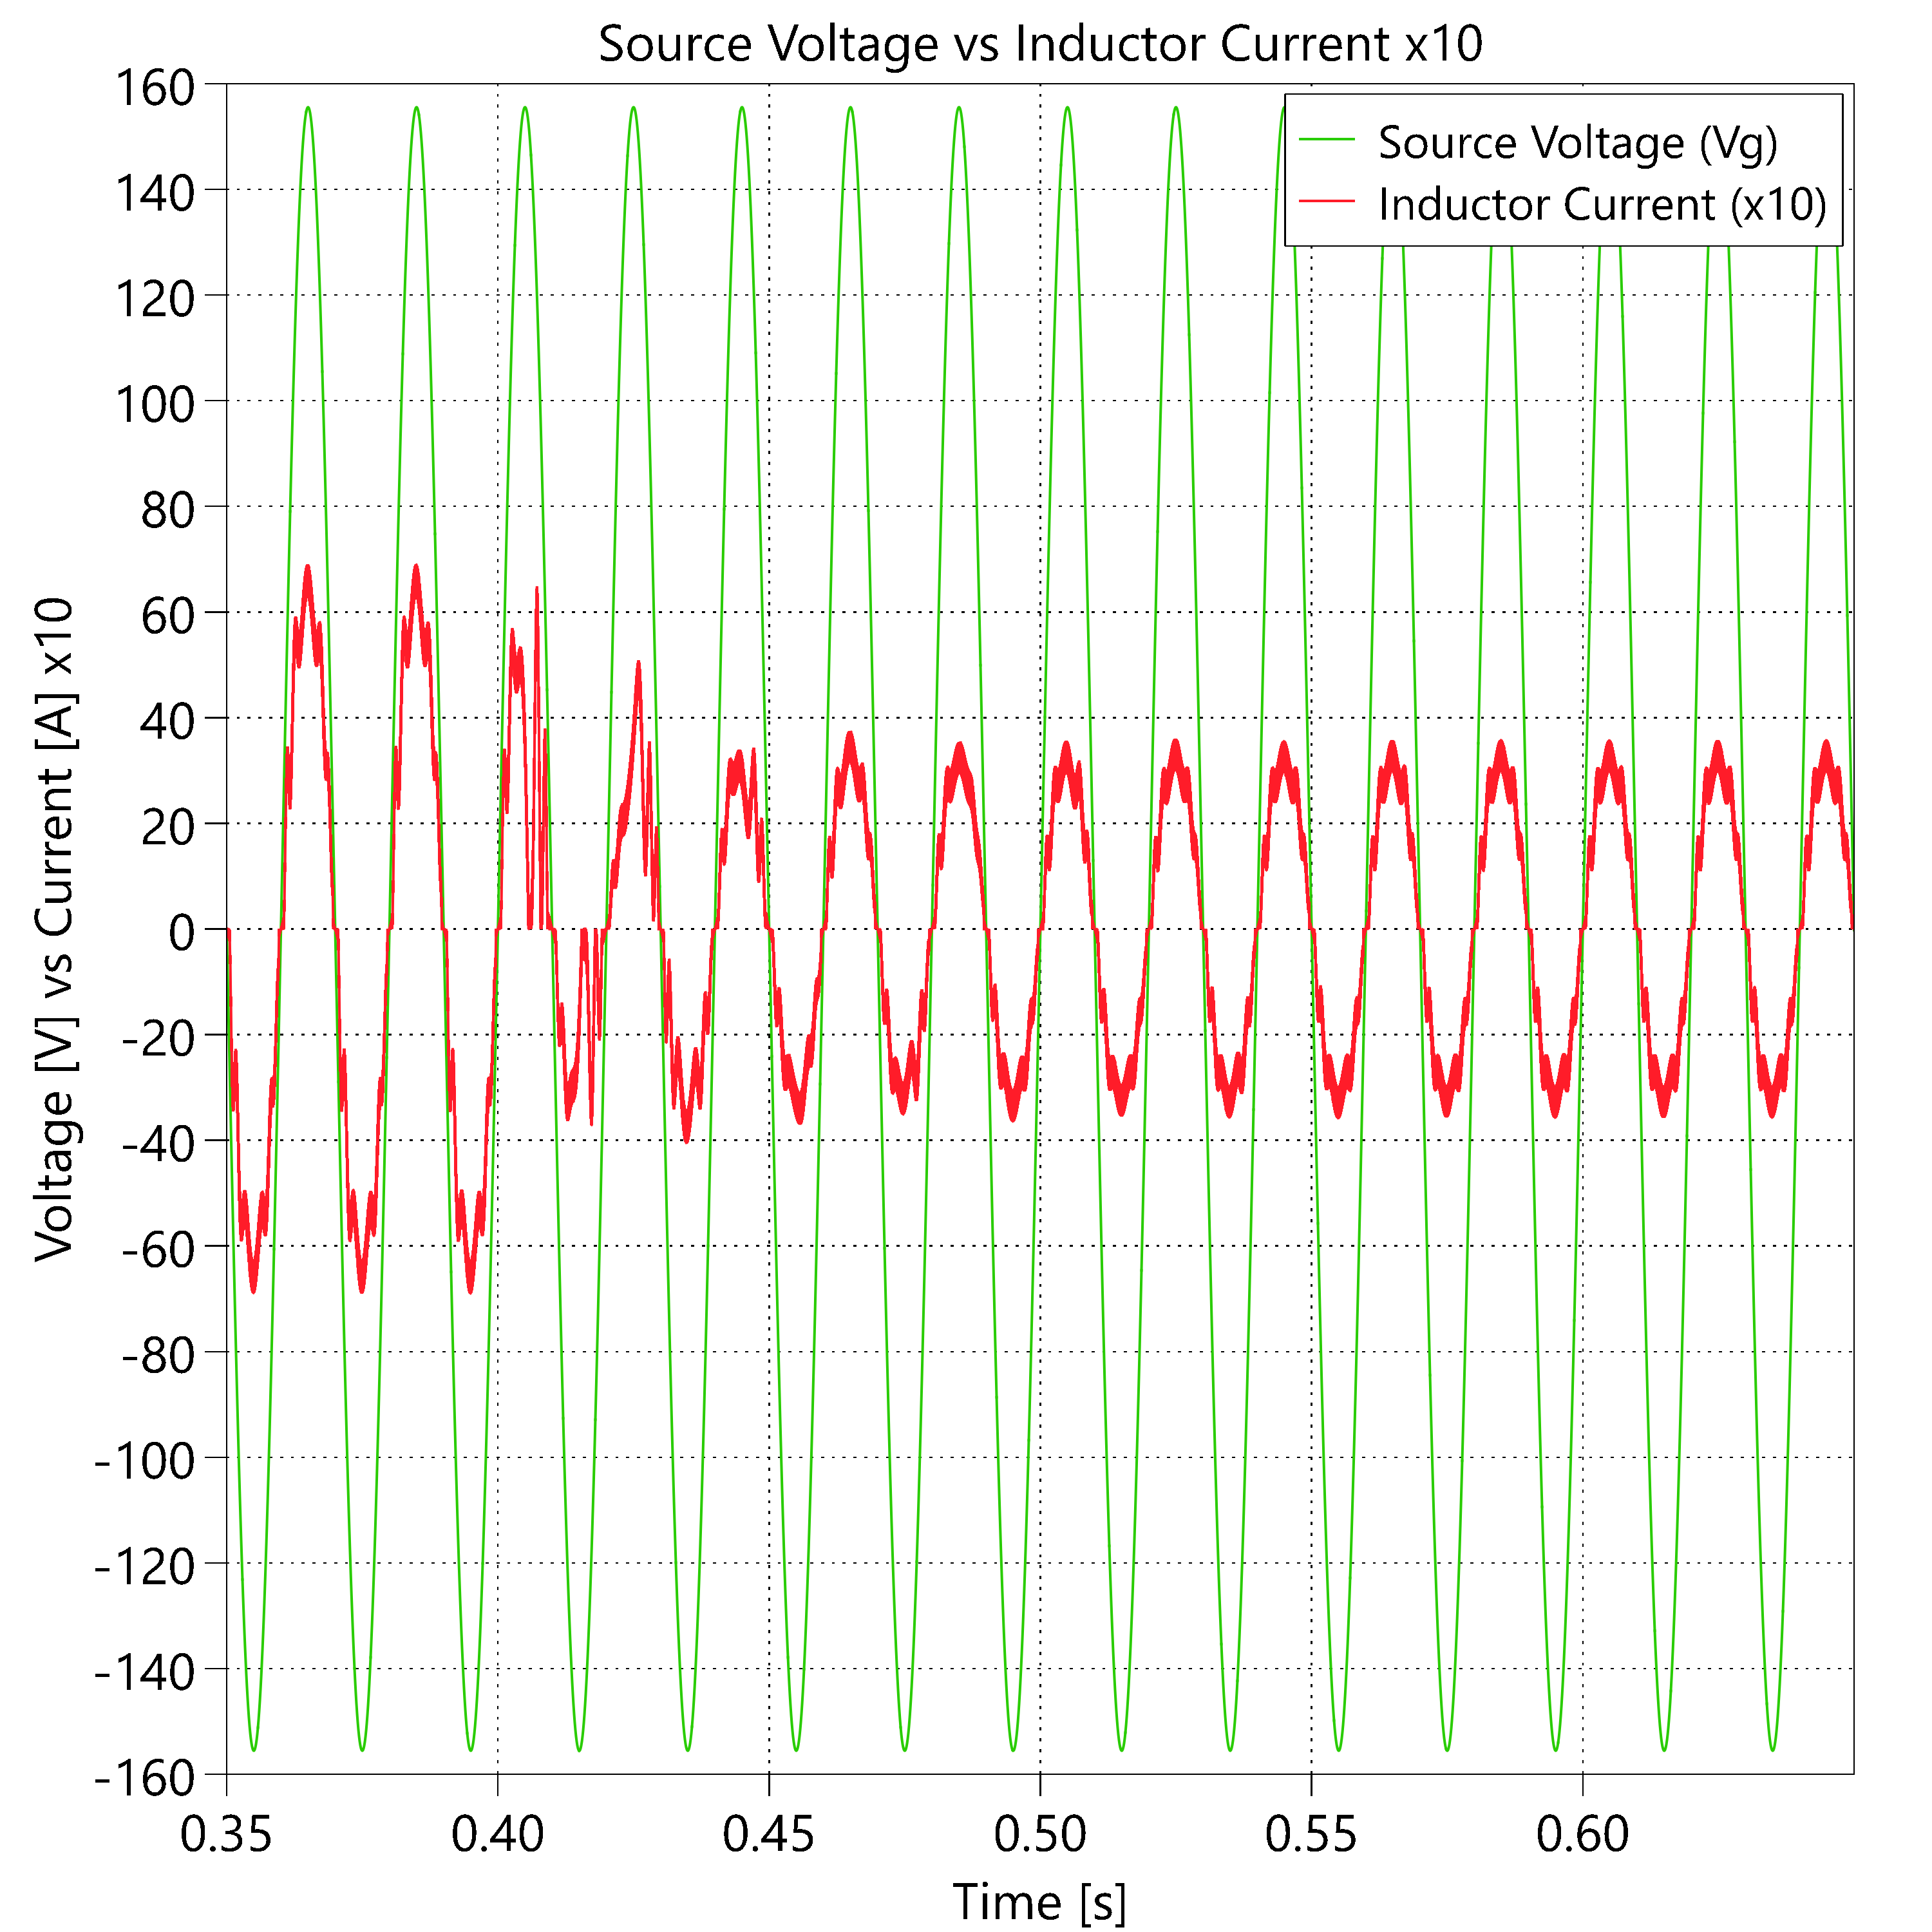
\includegraphics[width=1\linewidth]{figures/IL_phas_no_Xa_ref.png}
        \caption{Phasor Domain Control}
        \label{fig:duty_cycle_phasors}
    \end{subfigure}% <--- This % kills the hidden space!
    \caption{Input Voltage vs. Inductor Current Simulation Results}
    \label{fig:current_results}
\end{figure*}
% 
% Thus, while Lyapunov-based control theoretically offers global stability, as proved by the graph of the derivative of the Lyapunov energy function $\dot{V}(e)$, shown in Fig. \ref{fig:dV_dt_LY}, its application here highlights a critical limitation. The exceptionally poor transient performance suggests that the non-linear Lyapunov controller is highly sensitive to the perturbation caused by operating point changes, leading to the oscillations observed. 

\begin{table}[htp]
    \centering
    \caption{Settling Time, Voltage Overshoot vs. Inner Gain $K_c$}
    \label{tab:Lyapunov_Transient}
    \pgfplotstabletypeset[normal,
        columns/Kc/.style={column name={\textbf{$K_c$ Value}}},
        columns/SettlingTime/.style={column name={\textbf{Settling Time}}},
        columns/Overshoot/.style={column name={\textbf{Voltage Overshoot}}}
    ]{ %
    Kc                & SettlingTime  & Overshoot \\
    {$0.2$}           & {73 ms}     & {7 \%} \\
    {$0.02$}          & {73 ms}     & {7.2 \%} \\
    {$0.002$ (Nominal)}           & {64 ms}     & {7.2 \%} \\
    {$0.0002$}           & {-}     & {9.6 \%} \\
    }
\end{table}
Next, we compare the inductor current waveform, specifically inspecting the distortion introduced by the control strategies, and the power quality achieved. The performance of each model is reported in Table \ref{tab:Power_Quality}. 
The resulting current waveforms obtained from the simulations are shown in Fig. \ref{fig:current_results}. 
The PI/PR control strategy achieves excellent Power Factors exceeding 0.99 and maintains inductor current THD levels at or below $10\%$ across both load conditions. The Phasors Domain controller, in particular, demonstrates the most consistent and robust tracking, maintaining a PF of 0.994 under both load conditions. Conversely, the Lyapunov control strategy exhibits a significantly degraded steady-state performance profile. Under nominal operating conditions, it yields an unsatisfactory THD of $17\%$ at full load, which escalates to $25\%$ at light load. The corresponding Power Factor drops from 0.985 at $125 \Omega$, to a substandard 0.968 at $250 \Omega$. Such elevated input current distortion deviates fundamentally from the primary objective of any PFC converter. 
\begin{table}[htp]
    \centering
    \caption{Inductor Current THD and Power Factor (PF) Comparison}
    \label{tab:Power_Quality}
    \pgfplotstabletypeset[normal,
        columns/Parameter/.style={column name={\textbf{Parameter}}},
        columns/Value/.style={column name={\textbf{Value}}}
    ]{ %
    Parameter              & Value \\
    \topmidheader{2}{Lyapunov Control ($K_c = 0.002$)}
    {THD}          & {$17\%\space@\space R_o = 125\Omega;\quad 25\%\space@\space R_o = 250\Omega $ } \\ 
    {PF}    & {$0.985\space@\space R_o = 125\Omega;\quad 0.968\space@\space R_o = 250\Omega $} \\ 
    \midheader{2}{PI/PR Control}
    {THD}          & {$8\%\space@R_o = 125\Omega;\quad \space9.5\%\space@\space R_o = 250\Omega$} \\
    {PF}    & {$0.996\space@\space R_o = 125\Omega;\quad 0.995\space@\space R_o = 250\Omega$ } \\
    \midheader{2}{Phasor Domain Control}
    {THD}          & {$8\%\space@\space R_o = 125\Omega;\quad 10\%\space@\space R_o = 250\Omega$ } \\
    {PF}    & {$0.994\space@\space R_o = 125\Omega;\quad0.994\space@\space R_o = 250 \Omega$}  \\
    }
\end{table}
It indicates that the applied non-linear control law struggles to force the inductor current to accurately track the rectified sinusoidal reference during steady-state operation, leading to unacceptable harmonic distortions.
The underlying cause of this performance deficit is heavily implied by the sensitivity analysis presented in Table \ref{tab:Lyapunov_PowerQuality}, which evaluates the Power Factor against variations in the inner current loop gain, $K_c$. The data demonstrates that the system's performance is extremely sensitive to this specific parameter.



\begin{table}[htp]
    \centering
    \caption{Inductor Current, Power Factor vs. Inner Gain $K_c$}
    \label{tab:Lyapunov_PowerQuality}
    \pgfplotstabletypeset[normal,
        columns/Kc/.style={column name={\textbf{$K_c$ Value}}},
        columns/PF1/.style={column name={\textbf{PF  ($Ro = 125\Omega$)}}},
        columns/PF/.style={column name={\textbf{PF ($Ro = 250\Omega$)}}}
    ]{ %
    Kc                & PF1           & PF \\
    {$0.2$}           & {0.988}   & {0.973} \\
    {$0.02$}          & {0.988}   & {0.969} \\
    {$0.002$ (Nominal)} & {0.985}   & {0.968} \\
    {$0.0002$}           & {0.873}   & {0.804} \\
    }
\end{table}

\subsection{Impact of Feedforward Action}
\begin{figure*}[htbp]
    \centering
    \begin{subfigure}[b]{0.3\textwidth}
        \centering
        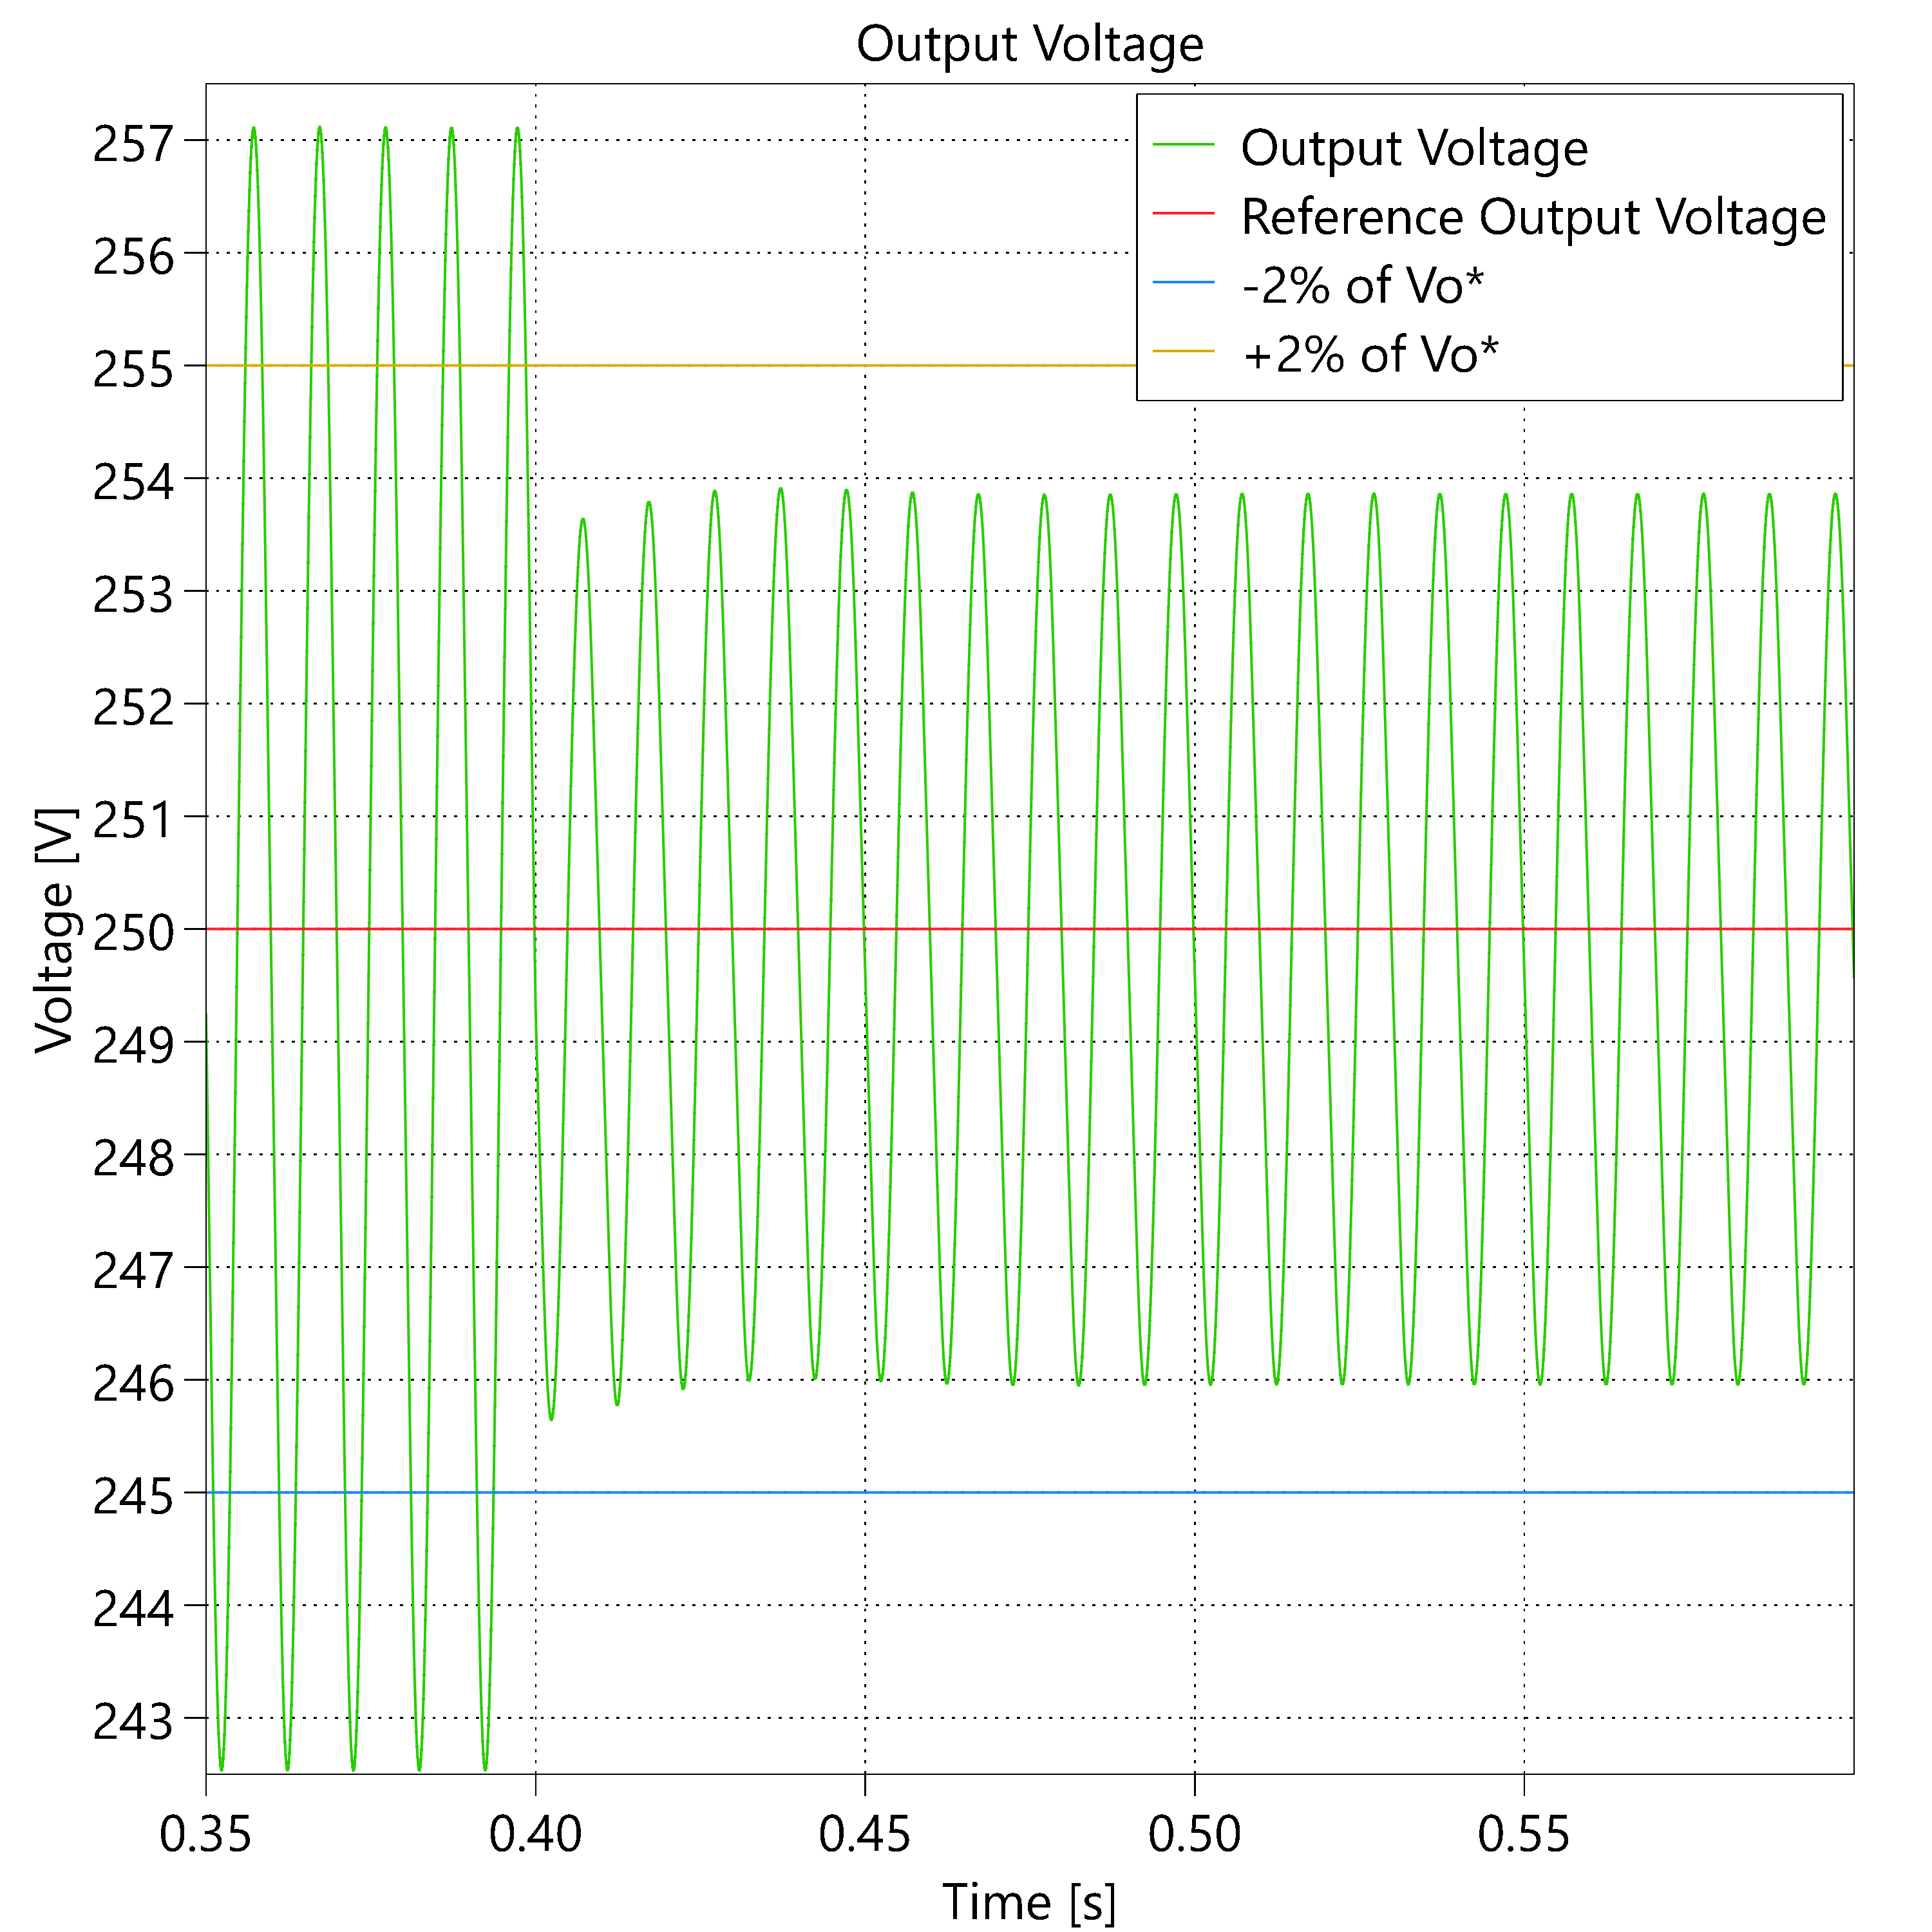
\includegraphics[width=\textwidth]{figures/V0_Lyapunov_x_alfa.png}
        \caption{Lyapunov-based Control, Output Voltage Regulation with $x_{\alpha_{ff}}$}
        \label{fig:LY_Vo_Xa}
    \end{subfigure}% <--- This % kills the hidden space!
    \hfill
    \begin{subfigure}[b]{0.3\textwidth}
        \centering
    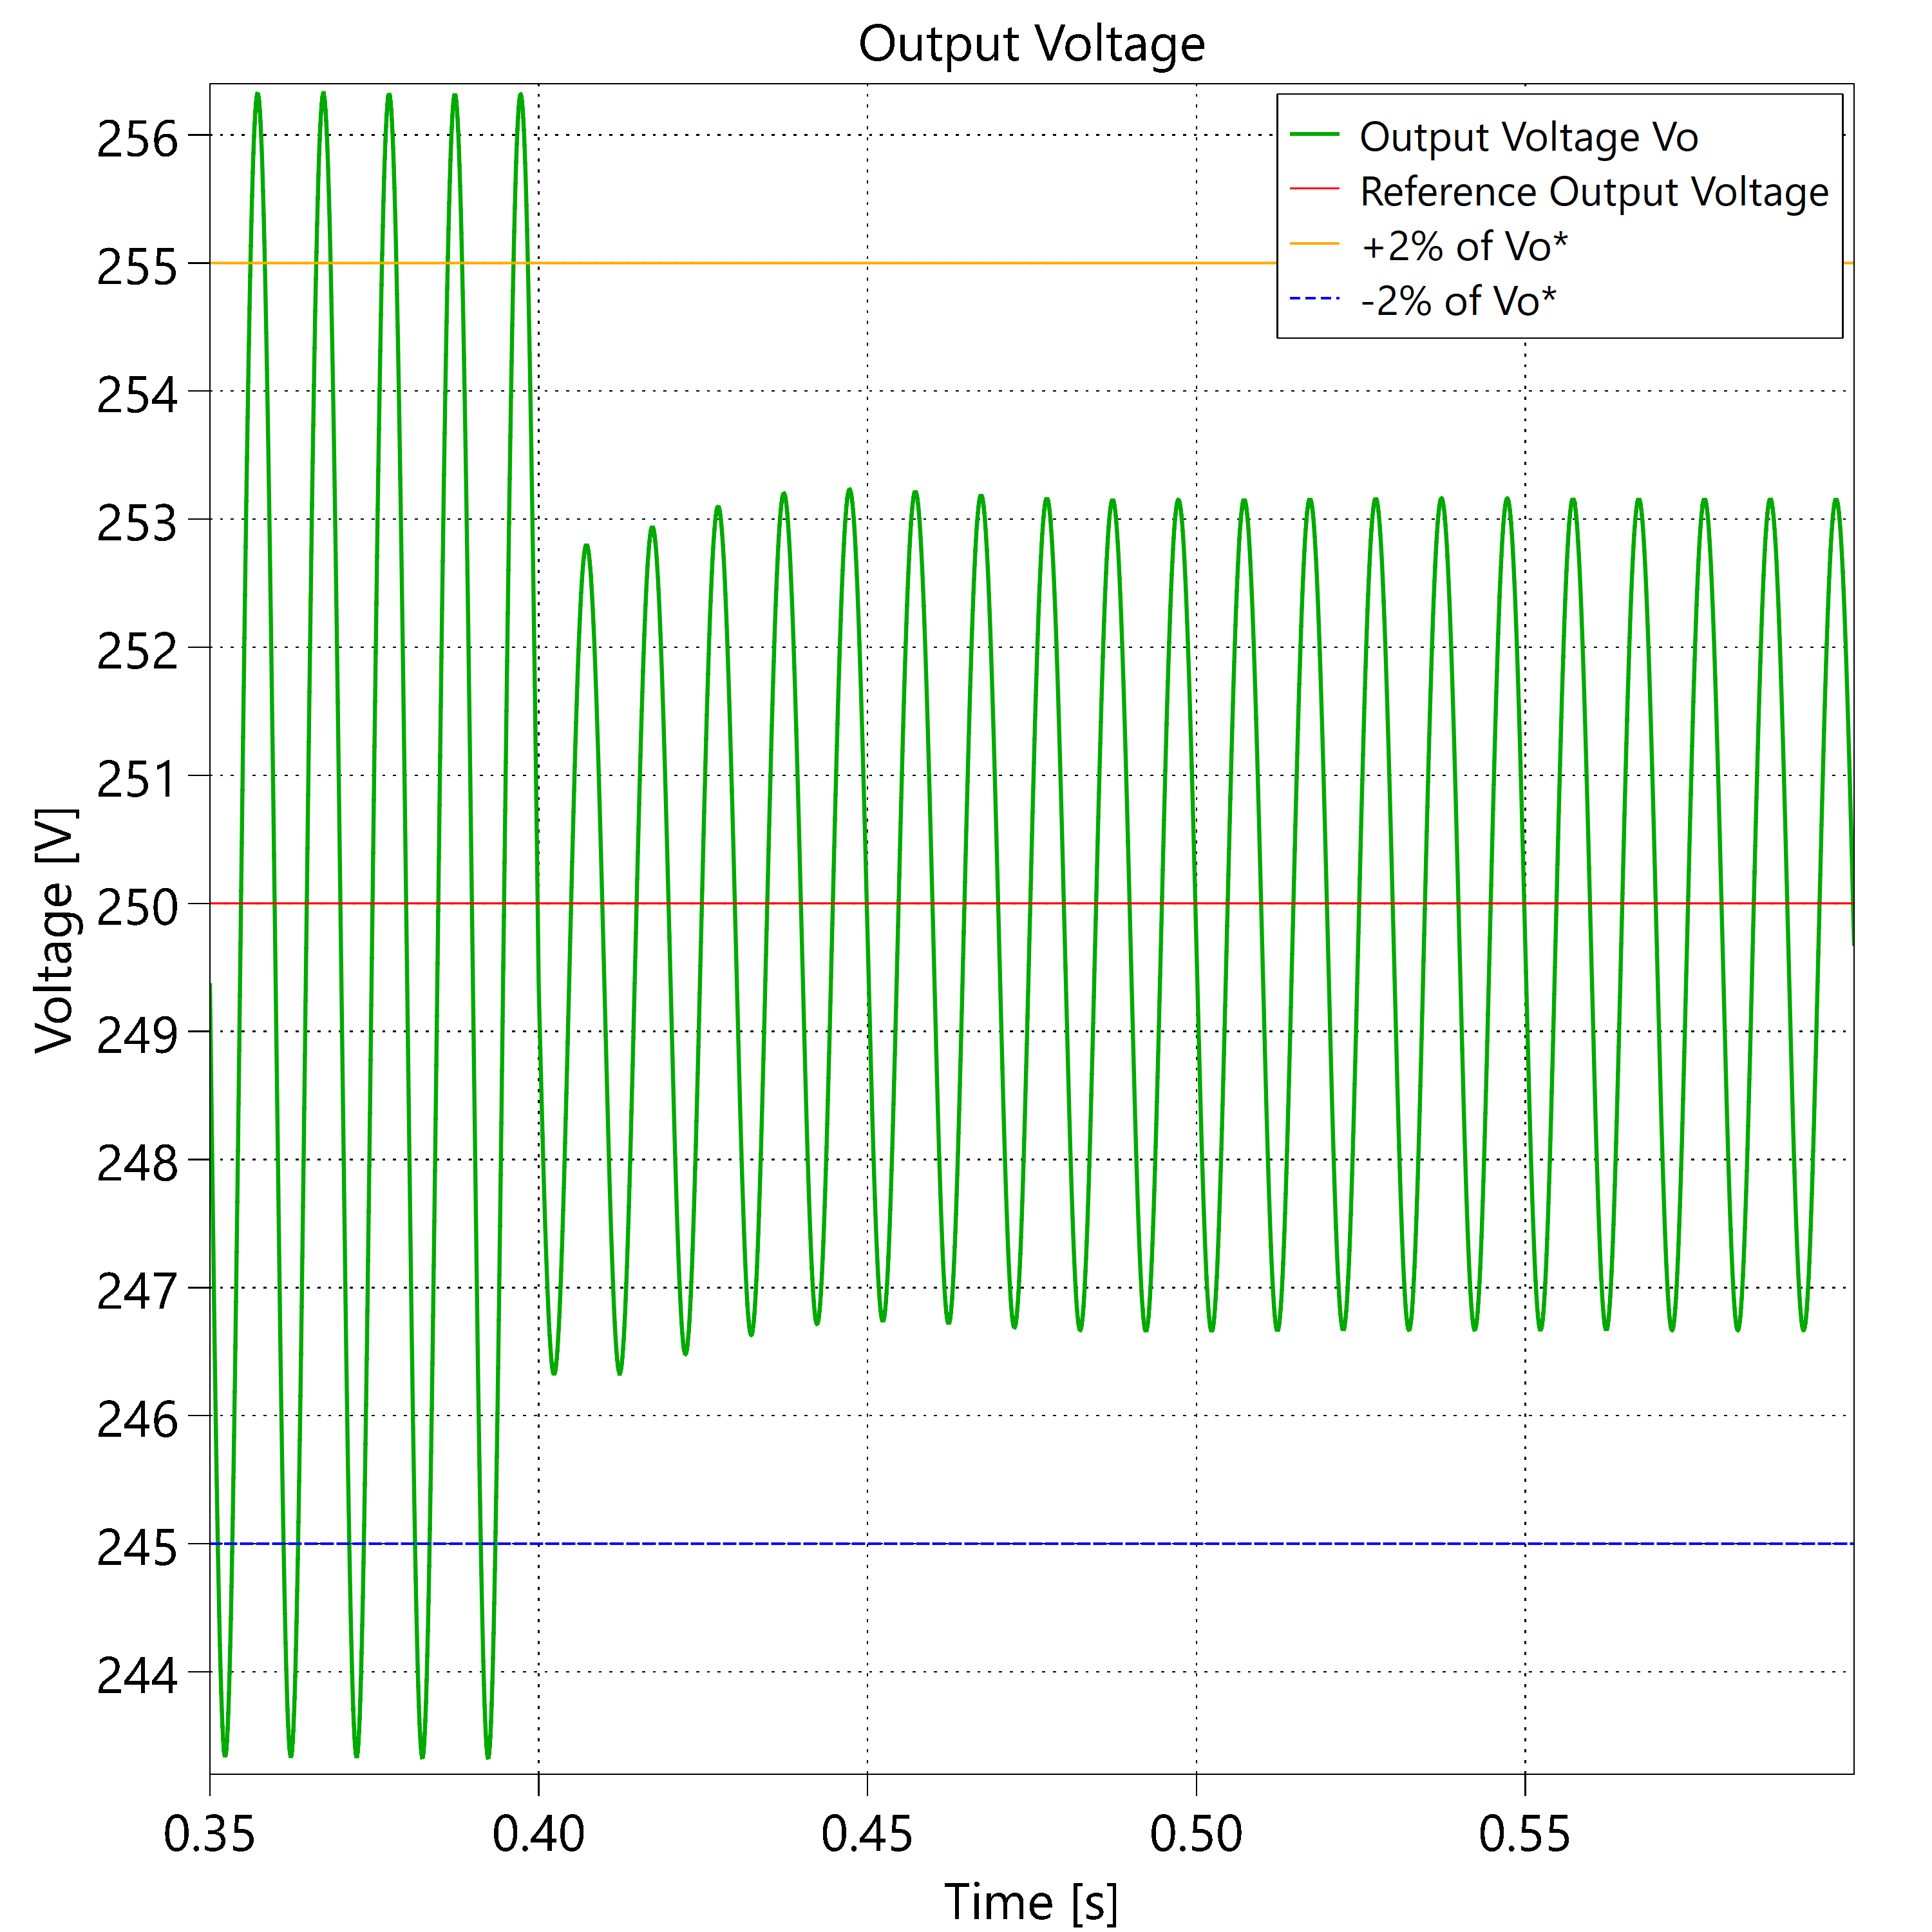
\includegraphics[width=1\linewidth]{figures/Vo_pipr_with_x_alpha.png}
        \caption{PI/PR Control, Output Voltage Regulation with $x_{\alpha_{ff}}$}
        \label{fig:PI_PR_Vo_Xa}
    \end{subfigure}% <--- This % kills the hidden space!
    \hfill
    \begin{subfigure}[b]{0.3\textwidth}
        \centering
    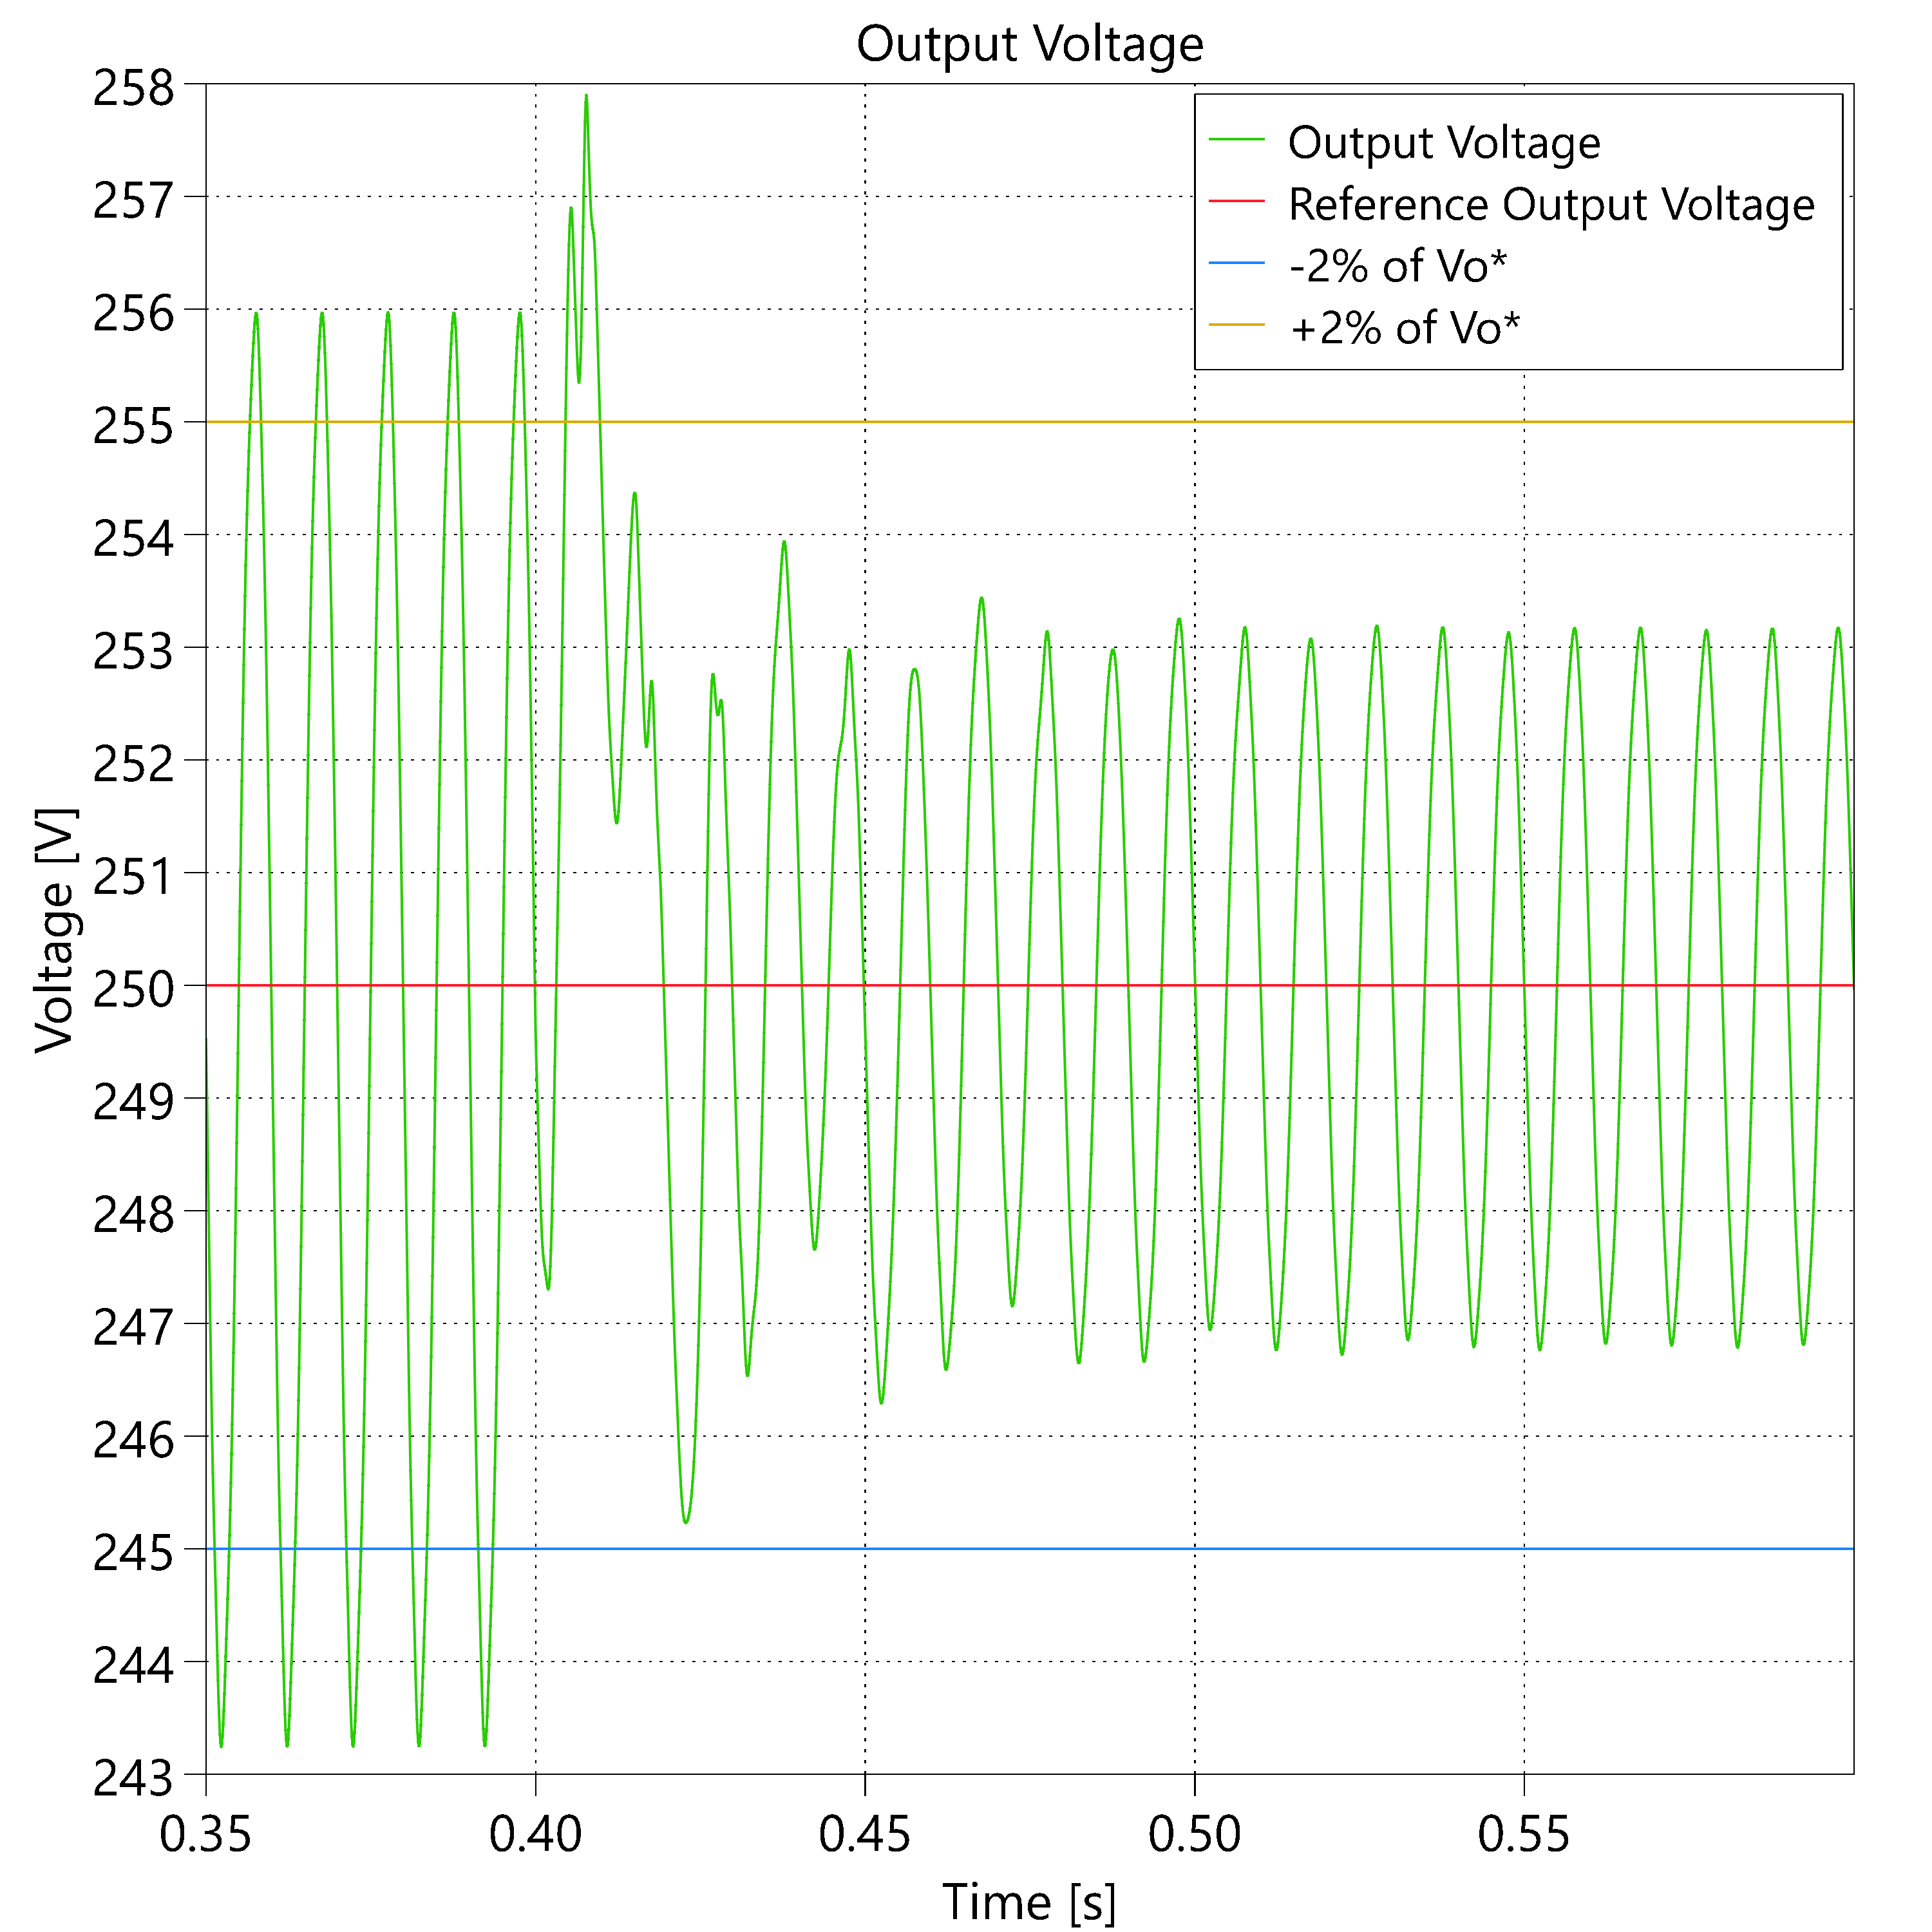
\includegraphics[width=1\linewidth]{figures/Vo_phas_Xa.png}
        \caption{Phasor Domain Control, Output Voltage Regulation with $x_{\alpha_{ff}}$}
        \label{fig:phVoXa}
    \end{subfigure}% <--- This % kills the hidden space!
    \caption{Feedforward Control Simulation Results}
    \label{fig:output_voltage_ff}
\end{figure*}
To evaluate the effectiveness of the load feedforward compensation, the dynamic response of the output voltage was analyzed under aload step at $t = 400\text{ms}$, both with and without the inclusion of the feedforward term ($x_{\alpha ff}$). 

Figure \ref{fig:voltage_noXa} illustrates the output voltage regulation strictly relying on the feedback loops, without feedforward action. Both the Lyapunov-based and PI/PR control strategies suffer massive voltage overshoots, peaking at approximately $269\text{ V}$ and $267\text{ V}$, respectively. These spikes violate the $\pm 2\%$ tolerance band. Instead, the Phasor Domain controller exhibits a better response, though still experiences a small deviation, peaking near $258\text{ V}$.

% Conversely,
Figure \ref{fig:output_voltage_ff} demonstrates the performance enhancement achieved by introducing the load feedforward term ($x_{\alpha ff}$). By mathematically decoupling the load disturbance from the feedback control effort, the system anticipates the sudden power demand rather than waiting for a voltage error to accumulate. 

The visual comparison confirms that the feedforward action practically eliminates the transient spikes across all three control architectures. For the Lyapunov and PI/PR controllers, the overshoots are entirely suppressed, as shown in Fig. \ref{fig:LY_Vo_Xa} and \ref{fig:PI_PR_Vo_Xa}, respectively. The voltage remains strictly confined within the $\pm 2\%$ boundary, achieving instantaneous settling. Nevertheless, the Phasor Domain controller exhibits equally robust disturbance rejection, but maintains the previously observed $258\text{ V}$ peak, as shown in Fig. \ref{fig:phVoXa}. 

% Ultimately, these results confirm that while standard feedback controllers are sufficient for steady-state operation, augmenting the control architecture with a feedforward action is strictly necessary to decouple load disturbances and ensure strict voltage regulation during severe transient events.



% \begin{table}[htp]
%     \centering
%     \caption{Comprehensive Performance Metrics of the Phasors Domain Approach}
%     \label{tab:phasors_performance}
%     \pgfplotstabletypeset[normal,
%         columns/Parameter/.style={column name={\textbf{Parameter}}},
%         columns/Value/.style={column name={\textbf{Value}}}
%     ]{ %
%     Parameter               & Value \\
%     \topmidheader{2}{Phasors Domain Control}
%     {Ripple, $\Delta V$}   & {$6V @ R_o = 125\Omega; 3.3V @ R_o = 250\Omega$} \\
%     {Settling Time, $t_s$} & {$9$ms} \\
%     {Overshoot, $OS\%$}      & {$3$\%} \\
%     {THD}           & {$8\% @ 125\Omega$; 10\% @ $250\Omega$} \\
%     {PF}     & {$0.994\space@\space R_o = 125\Omega; 0.994\space@\space R_o = 250\Omega$} \\
%     }
% \end{table}



% \subsection{Comparative analysis of stationary reference frame vs rotating reference frame }
% It has to be noted that, while the two stationary reference frame control strategies (Lyapunov-based and PI/PR control) are based on the same outer voltage loop PI parameter gains, the control method in the phasors domain uses different values for this purpose, because the PI compensation in this case affects only the active part of the power. Although the outer loop control structure is similar across the three control methods, the same PI parameter gains cannot be used to make the system work regardless of the control strategy; the PI controller has to be tuned differently in the phasors domain approach with respect to the stationary reference frame control methods. Therefore, each controller has been independently optimized to its own mathematical plant. Nonetheless, comparing the results obtained is still useful to get a rough idea of which control strategy achieves the best performance. 

% The key performance indicators for both output voltage regulation and input current quality have been quantified and are summarized in Table \ref{tab:res_voltage} and Table \ref{tab:res_current}.

% % \begin{table}[htp]
% %     \centering
% %     \caption{Output Voltage Regulation Performance ($\Delta V$, $t_s$, $OS\%$)}
% %     \label{tab:res_voltage}
% %     \pgfplotstabletypeset[normal,
% %         columns/Strategy/.style={string type, column name={\textbf{Control Strategy}}},
% %         columns/Ts/.style={string type, column name={\textbf{$t_s$}}},
% %         columns/OS/.style={string type, column name={\textbf{$OS\%$}}}
% %     ]{ %
% %     Strategy                & Ts           & OS \\
% %     {Lyapunov Control}      & {$183$ms} & {$9.2$\%} \\
% %     {PI/PR Control}         & {$82$ms}  & {$6.4$\%} \\
% %     {Phasor Domain Control} & {$9$ms}   & {$3.0$\%} \\
% %     }
% % \end{table}

% The quantitative data confirms the steady-state limitations of the implemented Lyapunov strategy. While its voltage ripple is acceptable, it fails to adequately shape the input current, resulting in a THD of $17\%$ at nominal load that degrades to an unacceptable $25\%$ at $250\Omega$. Consequently, its Power Factor drops to $0.968$ under light load conditions, rendering it the least effective strategy for meeting stringent power quality regulations.

% % \begin{table}[htp]
% %     \centering
% %     \caption{Inductor Current Performance (THD, PF)}
% %     \label{tab:res_current}
% %     \pgfplotstabletypeset[normal,
% %         columns/Strategy/.style={string type, column name={\textbf{Control Strategy}}},
% %         columns/PF1/.style={string type, column name={\textbf{PF ($125\Omega$)}}},
% %         columns/PF2/.style={string type, column name={\textbf{PF ($250\Omega$)}}}
% %     ]{ %
% %     Strategy                & PF1       & PF2 \\
% %     {Lyapunov Control}      & {$0.985$} & {$0.968$} \\
% %     {PI/PR Control}         & {$0.996$} & {$0.995$} \\
% %     {Phasor Domain Control} & {$0.994$} & {$0.994$} \\
% %     }
% % \end{table}

\section{Conclusions}

This study provided a comprehensive comparative evaluation of three distinct control strategies for the Bridgeless Boost PFC Converter (BBC): Lyapunov-based control, Cascaded PI/PR control, and Phasor Domain control. The experimental results, obtained via PLECS simulations, highlight significant trade-offs between dynamic agility, steady-state stability, and power quality. In particular, it turned out that although the Lyapunov-based control offers theoretical global stability and a fast recovery time (64ms), it  struggles to completely eliminate the phase and amplitude error on the sinusoid, leading to higher harmonic distortion (THD of 17-25) in the input current and it shows a significant sensitivity to the gain parameter $K_c$ (because if it is low, the system is slow, while if it is high the duty cycle becomes "noisy"). On the other hand, the cascade PI/PR control proved to be the most balanced solution because, although its transient response ($82$ms) is slower than the other methods, it excels in its primary goal, achieving a Power Factor (PF) of 0.996 and a low THD (8\%). Finally, the Phasor Domain control, by mapping AC variables into a rotating DC-equivalent frame, it exhibits the lowest voltage ripple ($5.6$V at full load) and the fastest settling time ($10$ms).  
The introduction of the load feedforward term provided a significant improvement across all architectures. By anticipating power demands rather than reacting to voltage errors, the system effectively decoupled load disturbances from the feedback effort.
In conclusion, while the PI/PR control remains the standard for its simplicity and power quality, the Phasor Domain control represents the superior choice for high-performance applications where transient agility is critical. The addition of feedforward action is highly recommended for all strategies to ensure grid stability and voltage regulation under severe load variations.

%	REFERENCE LIST
%----------------------------------------------------------------------------------------
\begin{thebibliography}{15} % Updated to 15 to accommodate new entries

% --- Your Original References ---
\bibitem{survey_topologies}
Ortiz-Castrillón, J.R.; Mejía-Ruíz, G.E.; Muñoz-Galeano, N.; López-Lezama, J.M.; Saldarriaga-Zuluaga, S.D. PFC Single-Phase AC/DC Boost Converters: Bridge, Semi-Bridgeless, and Bridgeless Topologies. Appl. Sci.2021.\url{https://doi.org/10.3390/app11167651}

\bibitem{TU} O. Gulbudak, M. Gokdag and M. F. Özlük, "Performance Evaluation of Lyapunov Control Method for Bridgeless Boost PFC," 2024 IEEE 3rd Industrial Electronics Society Annual On-Line Conference (ONCON), Beijing, China, 2024, pp. 01-06. \url{https://ieeexplore.ieee.org/document/10931554}

\bibitem{MG} M. Gopinath, Prabakaran and S. ramareddy, "A brief analysis on bridgeless boost PFC converter," International Conference on Sustainable Energy and Intelligent Systems (SEISCON 2011), Chennai, 2011, pp. 242-246. \url{https://ieeexplore.ieee.org/document/6143316}

\bibitem{pr_pfc}
S. Oprea, C. Radoi and A. Florescu, ``Single-phase power factor correction circuit with Proportional-Resonant control,`` in \emph{Proceedings of the 2014 6th International Conference on Electronics, Computers and Artificial Intelligence (ECAI), Bucharest, Romania}, 2014, pp. 7-10, doi: 10.1109/ECAI.2014.7090155 \url{https://ieeexplore.ieee.org/document/7090155}

\bibitem{pr_control}
Teodorescu, Remus and Frede Blaabjerg. ``Proportional-Resonant Controllers. A New Breed of Controllers Suitable for Grid-Connected Voltage-Source Converters.`` (2004) \url{https://www.google.com/url?sa=t&source=web&rct=j&opi=89978449&url=http://www.jee.upt.ro/index.php/jee/article/download/WL1151672308W44a51ff4512f9/67&ved=2ahUKEwiOl4Kw14CUAxVHgv0HHfJ0HC4QFnoECBkQAQ&usg=AOvVaw2kS4FyemdwGo-uheDBWjvQ}

\bibitem{totem_pole_dq}
C. -Y. Tang and D. -D. Shih, ``A Single-Phase Totem-Pole Converter with Four Quadrants Active and Reactive Power Control by Using the Direct-Quadrature Control,`` in \emph{13th International Conference on Renewable Energy Research and Applications (ICRERA), Nagasaki, Japan}, 2024, pp. 1330-1335, doi: 10.1109/ICRERA62673.2024.10815440. \url{https://ieeexplore.ieee.org/document/10815440}

\bibitem{lyapunov_pr}
H. Komurcugil, N. Altin, S. Ozdemir and I. Sefa, ``Lyapunov-Function and Proportional-Resonant-Based Control Strategy for Single-Phase Grid-Connected VSI With LCL Filter,`` in \emph{IEEE Transactions on Industrial Electronics, vol. 63, no. 5, pp. 2838-2849}, May 2016, doi: 10.1109/TIE.2015.2510984. \url{https://ieeexplore.ieee.org/document/7369986}

\bibitem{GitHub} Please find the PLECS models analysed in this study at the following link: \url{https://github.com/Struffoli11/DCSES_BRIDGELESS_BOOST_PFC_CONVERTER}.

\bibitem{PLECS} PLECS Bridgeless Boost PFC Converter Demo Model. \url{https://www.plexim.com/sites/default/files/demo_models_categorized/plecs/bridgeless_boost_pfc_converter.pdf}

\bibitem{PLL} PLECS Single-Phase PLL, pp. 847-850. \url{https://www.plexim.com/sites/default/files/plecsmanual.pdf} 








\end{thebibliography}

%----------------------------------------------------------------------------------------



%----------------------------------------------------------------------------------------
%	APPENDIX CONTEXT
%----------------------------------------------------------------------------------------
\newpage
\textbf{ }
\newpage
\section*{Appendix A}
The Bridgeless Boost PFC converter is inherently a time-varying non-linear system. Because the input voltage $v_g(t)$ (and therefore $\text{sgn}(v_g)$) and the duty cycle $d(t)$ vary continuously over the grid cycle, a standard Linear Time-Invariant (LTI) small-signal model cannot be strictly applied.
The transfer functions, however, can be derived from the linearized state-space small-signal model. To do that, the system is frozen at the peak of the grid voltage ($\theta = \omega t =\dfrac{\pi}{2}+ 2k\pi$ where $k\in 
\mathbb{Z}$) to derive quasi-static worst-case transfer functions since the system dynamics change with time, 

Since when the grid voltage is positive, and at peak we have a positive zero, this is the worst case for the control design. The poles of the system are the same for the positive and negative semiperiod.
Therefore, even if the transfer functions are time-varying, we proceed to consider the transfer functions for the worst case.\\

With this assumption, we can write the following:
\begin{align*}
v_g(t) &= V_g \\
\operatorname{sgn}(v_g(t))&=1 \\
u_o(t) &= D\\
D'&=1-D\\
\Delta{d} &= d - D
\end{align*}
These conditions allow to write $A(t) = A$ and $B_d(t) = B_d$ in the linearized small signal model, which yields the following:
{\small
\begin{equation}
\Delta{X}(s) = (sI - A)^{-1} B_d \Delta{d}(s) + (sI - A)^{-1} B_v \Delta{V}_g(s)
\end{equation}
}
where $(sI-A)^{-1}$ and $\Delta(s)$ are expressed as:
{\small
\begin{equation}
\begin{aligned}
(sI - A)^{-1} &= \frac{1}{\Delta(s)}
\begin{pmatrix} 
s + \dfrac{1}{R_0 C} & -\dfrac{D'}{L} \\[12pt] 
\dfrac{D'}{C} & s + \dfrac{r_f}{L} 
\end{pmatrix} \\[20pt]
\Delta(s) &= s^2 + s \left[ \frac{r_f R_0 C + L}{R_0 L C} \right] + \frac{(D')^2 R_0 + r_f}{R_0 L C}
\end{aligned}
\end{equation}
}

{\small
Below are reported all the transfer functions that describe the entire system:
\begin{equation}\label{eq:Control-to-Output Voltaage Transfer Function}
G_{vd}(s) = \frac{\dfrac{\mathrm{V_g} R_0}{(R_0 (D')^2 + r_f)^2} \Big[ R_0 (D')^2 - r_f - sL \Big]}{\dfrac{R_0 LC}{(D')^2 R_0 + r_f} s^2 + s \left( \dfrac{r_f R_0 C + L}{(D')^2 R_0 + r_f} \right) + 1}
\end{equation}
}
It is possible to rewrite the Control-to-Output Voltage Transfer Function Eq. (\ref{eq:Control-to-Output Voltaage Transfer Function}), in terms of the gain $K_{vd}$, the damping factor $\zeta$,  the natural pulsation $\omega_n$ and the RPH (Right Half Plane) $\omega_z$ (or in other words the so called non minimum phase zero that corresponds to a system whose response to an input exhibits non-monotonic behavior, often characterized by an initial response in the opposite direction of the intended output).

\begin{equation}
G_{vd}(s) = K_{vd} \frac{\left( 1 - \frac{s}{\omega_z} \right)}{\frac{s^2}{\omega_n^2} + \frac{2\zeta s}{\omega_n} + 1}
\end{equation}

\begin{equation}
\omega_z = \frac{R_0 (D')^2 - r_f}{L}
\end{equation}

\begin{equation}
K_{vd} = \frac{\mathrm{V_g} R_0}{(R_0 (D')^2 + r_f)^2} \left[ R_0 (D')^2 - r_f \right]
\end{equation}

\begin{equation}
\omega_n = \sqrt{\frac{(D')^2 R_0 + r_f}{R_0 L C}}
\end{equation}

{\small
\begin{equation}
\begin{split}
\zeta &= \frac{1}{2} \frac{r_f R_0 C + L}{(D')^2 R_0 + r_f} \sqrt{\frac{(D')^2 R_0 + r_f}{R_0 L C}} = \\
      &= \frac{1}{2\omega_n} \left( \frac{r_f}{L} + \frac{1}{R_0 C} \right)
\end{split}
\end{equation}
}
The same strategy is applied to the Control-to-Inductor Current Transfer Function:

{\small
\begin{equation}
G_{id}(s) = \frac{\dfrac{2\mathrm{V_g} D' R_0}{((D')^2 R_0 + r_f)^2} \left( \dfrac{s R_0 C}{2} + 1 \right)}{\dfrac{R_0 L C}{(D')^2 R_0 + r_f} s^2 + s \left( \dfrac{r_f R_0 C + L}{(D')^2 R_0 + r_f} \right) + 1}
\end{equation}

\begin{equation}
G_{id}(s) = K_{id} \frac{\left( 1 + \dfrac{s}{\omega_z} \right)}{\dfrac{s^2}{\omega_n^2} + s \dfrac{2\zeta}{\omega_n} + 1}
\end{equation}

\begin{equation}
K_{id} = \frac{2 \mathrm{V_g} D' R_0}{((D')^2 R_0 + r_f)^2}
\end{equation}
\begin{equation}
\omega_z = \frac{2}{R_0 C}
\end{equation}

As for the Input-to-Output Voltage Transfer Function and to the Input-to-Inductor Current Transfer Function, they are represented, respectively, by Eq. (\ref{eq:Input-to-Output Voltage Transfer Function}) and (\ref{eq:Input-to-Inductor Current Transfer Function}):
{ \small
\begin{equation}\label{eq:Input-to-Output Voltage Transfer Function}
\begin{aligned}
G_{vv_g}(s) &=\frac{ \dfrac{R_o D'}{(D')^2 R_o + r_f} }{ \left( \dfrac{R_o CL}{(D')^2 R_o + r_f} \right)s^2 + s\left( \dfrac{r_f R_o C + L}{(D')^2 R_o + r_f} \right) + 1 }
\end{aligned}
\end{equation}
}
{\small
\begin{equation}\label{eq:Input-to-Inductor Current Transfer Function}
G_{iv_g}(s) = \frac{\dfrac{sR_o C + 1}{(D')^2 R_o + r_f}}{\left( \dfrac{R_o LC}{(D')^2 R_o + r_f} \right) s^2 + s \left( \dfrac{r_f R_o C + L}{(D')^2 R_o + r_f} \right) + 1}
\end{equation}
}

Finally, the uncompensated voltage regulator loop transfer function, used in the outer loop in the Lyapunov-based and PI/PR control strategies, is defined as:
\begin{equation}
\begin{aligned}
T_{uv}(s)&=\frac{G_{vd}(s)}{G_{id}(s)}=\\
&= T_{uv_0} \cdot \frac{ 1 - \dfrac{s}{\omega_z} }{ 1 + \dfrac{s}{\omega_p} }
\end{aligned}
\end{equation}

where the parameters $\omega_z$, $\omega_p$ and $T_{uv_0}$ are expressed as:
\begin{equation} 
\begin{cases} 
\omega_p = \dfrac{2}{R_o C} \\[15pt] 
\omega_z = \dfrac{R_o (D')^2 - r_f}{L} \\[15pt] 
T_{uv_0} = \dfrac{R_o (D')^2 - r_f}{2 D'} 
\end{cases}
\end{equation}
\section*{Appendix B}
Starting from the steady-state equations in the phasors domain, we can write:
\begin{subequations}
\begin{align}
    L \frac{d\bar{x}_\alpha}{dt} &= -r_f \bar{x}_\alpha + \omega L \bar{x}_\beta + u_\alpha \\
    L \frac{d\bar{x}_\beta}{dt} &= -r_f \bar{x}_\beta - \omega L \bar{x}_\alpha + u_\beta
\end{align}
\end{subequations}

Taking the Laplace transform of the state equations yields:

\begin{align}
    (sL + r_f)\bar{X}_\alpha(s) &= \omega L \bar{X}_\beta(s) + U_\alpha(s) \\
    (sL + r_f)\bar{X}_\beta(s) &= -\omega L \bar{X}_\alpha(s) + U_\beta(s)
\end{align}

This system can be represented in Multiple-Input Multiple-Output (MIMO) matrix form as:
\begin{equation}
    \begin{bmatrix} sL+r_f & -\omega L \\ \omega L & sL+r_f \end{bmatrix} \begin{bmatrix} \bar{X}_\alpha(s) \\ \bar{X}_\beta(s) \end{bmatrix} = \begin{bmatrix} U_\alpha(s) \\ U_\beta(s) \end{bmatrix}
\end{equation}

By defining the state vector $Y(s) = [\bar{X}_\alpha(s), \bar{X}_\beta(s)]^T$, the input vector $U(s) = [U_\alpha(s), U_\beta(s)]^T$, and the inverse plant matrix $G^{-1}(s)$, we establish the open-loop relationship:
\begin{equation}
    Y(s) = G(s)^{-1}U(s) = P(s)U(s)
\end{equation}
where $P(s) = G(s)^{-1} = \begin{bmatrix} sL+r_f & -\omega L \\ \omega L & sL+r_f \end{bmatrix}^{-1}$.

To eliminate the cross-coupling ($\omega L$) terms, a state-feedback decoupling matrix $\Gamma_0(s)$ is introduced. The control law is defined as:
\begin{equation}\label{eq:appen_A}
    U(s) = V(s) - \Gamma_0(s)Y(s) 
\end{equation}
An alternative form of \ref{eq:appen_A}, is the following:
\begin{equation}
   U(s) = V(s) - \Gamma_0(s)P(s)U(s)
\end{equation}
where $V(s) = [V_\alpha(s), V_\beta(s)]^T$ represents the outputs of the standard PI compensators. Solving for $U(s)$ gives:
\begin{align}
    [I + \Gamma_0(s)P(s)]U(s) &= V(s) \\ U(s) &= [I + \Gamma_0(s)P(s)]^{-1}V(s)
\end{align}
Substituting this back into the plant equation yields the closed-loop transfer matrix:
\begin{equation}
    Y(s) = P(s)[I + \Gamma_0(s)P(s)]^{-1}V(s)
\end{equation}

We desire the resulting closed-loop system to be a completely decoupled, diagonal matrix $\Delta(s)$, where both axes behave as independent first-order systems:
\begin{equation}
    \Delta(s) = \begin{bmatrix} \Delta_{11}(s) & 0 \\ 0 & \Delta_{22}(s) \end{bmatrix} = \begin{bmatrix} \frac{1}{sL+r_f} & 0 \\ 0 & \frac{1}{sL+r_f} \end{bmatrix}
\end{equation}

Equating the closed-loop system to our target matrix $\Delta(s)$ allows us to solve for the required decoupling network $\Gamma_0(s)$:
{\small
\begin{align}
    P(s)[I + \Gamma_0(s)P(s)]^{-1} &= \Delta(s) \\
    \Delta(s)[I + \Gamma_0(s)P(s)] &= P(s) \\
    P(s) - \Delta(s) &= \Delta(s)\Gamma_0(s)P(s) \\
    \Gamma_0(s) &= \Delta^{-1}(s) - P^{-1}(s)
\end{align}
}
Substituting $\Delta^{-1}(s)$ and $P^{-1}(s) = G^{-1}(s)$ yields the final algebraic decoupling matrix:

\begin{equation}
     \Gamma_0(s) = \begin{bmatrix} 0 & \omega L \\ -\omega L & 0 \end{bmatrix}
\end{equation}
Substituting in \ref{eq:appen_A}, we get:

\begin{align}
   u_\alpha &= v_\alpha - \omega L \bar{x}_\beta\label{eq:u_alpha} \\
   u_\beta &= v_\beta + \omega L \bar{x}_\alpha\label{eq:u_beta}
\end{align}

\end{document}


% The comparative evaluation of the implemented control strategies reveals distinct operational trade-offs between transient agility, steady-state stability, and overall power quality. 
% The Phasor Domain control emerges as the most robust and highly performant architecture overall.
% Within the stationary reference frame, the conventional cascaded PI/PR control strategy proves to be the best solution. While its transient response to load steps is moderately slower compared to the other methods, like Lyapunov-based control, it excels in its primary objective: producing a grid current that is low-distorted and achieving optimal power factor. 
% Conversely, the non-linear Lyapunov-based approach demonstrates significant practical limitations despite its theoretical guarantee of global stability. While it achieves a relatively fast voltage recovery and tighter steady-state voltage bounds than the PI/PR controller, these benefits come at an unacceptable cost to power quality.
% Ultimately, while the standard PI/PR controller remains a good solution, the Phasor Domain approach provides a superior balance, delivering unmatched dynamic performance without sacrificing the strict power quality requirements of the PFC converter.
% The comparative performance, summarized in Table \ref{tab:comparison}, highlights these trade-offs. 
% Thus, we can conclude that:
% \begin{itemize}
%     \item \textbf{Lyapunov-based Control}
%     \begin{itemize}
%         \item \textit{Advantages:} Provides theoretical global asymptotic stability ($V(e) > 0, \dot{V}(e) < 0$) and remains robust against large input voltage variations.
%         \item \textit{Disadvantages:}: The irregular duty cycle increases the risk of Electromagnetic Interference (EMI).
%     \end{itemize}
    
%     \item \textbf{Cascaded PI/PR Control}
%     \begin{itemize}
%         \item \textit{Advantages:} Efficiently eliminates phase lag and tracking errors in the stationary frame. It simplifies system synthesis by treating the fast inner loop as a unity-gain block.
%         \item \textit{Disadvantages:} The resonant gain ($K_R$) is highly frequency-selective; performance degrades if the grid frequency deviates from the nominal 50Hz.
%     \end{itemize}

%     \item \textbf{Dynamic Phasors Approach}
%     \begin{itemize}
%         \item \textit{Advantages:} Maps AC variables to DC equivalents, allowing independent active and reactive power control. Decoupling effectively cancels cross-coupling between axes.
%         \item \textit{Disadvantages:} Significant computational overhead and high dependency on the PLL settling time.
%     \end{itemize}
% \end{itemize}